\chapter{The building blocks of the Finite Element Method} %%%%%%%%%%%%%%%%%%%%%%%%%%%%%%%%%%%%%%%%
\begin{flushright} {\tiny {\color{gray} chapter\_fem0.tex}} \end{flushright}

\section{A bit of FE terminology}\label{sec:terminology} \input{terminology} %------------------
\newpage
\section{Elements and basis functions in 1D}\label{sec:elts1D} \begin{flushright} {\tiny {\color{gray} elements1D.tex}} \end{flushright}


%------------------------------------------
\subsubsection{Linear basis functions ($Q_1$) \label{sec:bf1}}
\index{general}{$Q_1$}

Let $f(r)$ be a $C^1$ function on the interval $[-1:1]$ with $f(-1)=f_1$  and $f(1)=f_2$.
\begin{center}
\includegraphics[width=8cm]{images/linshapefct.png}
\end{center}
Let us assume that the function $f(r)$ is to be approximated on $[-1,1]$ by the first order polynomial 
\begin{equation}
f^h(r)=a+br \label{eqquad1}
\end{equation}
Then it must fulfil
\begin{eqnarray}
f^h(r=-1)&=&a-b =f_1 \nonumber\\
f^h(r=+1)&=&a+b =f_2 \nonumber
\end{eqnarray}
This leads to  
\begin{eqnarray}
a&=&\frac{1}{2}(f_1+f_2)  \nn\\
b&=&\frac{1}{2}(-f_1+f_2)  
\end{eqnarray}
and then replacing $a,b$ in Eq.~\eqref{eqquad1} by the above values one gets
\[
f^h(r) = \left[  \frac{1}{2}(1-r)\right] f_1 + \left[ \frac{1}{2}(1+r) \right] f_2
\]
or
\[
f^h(r)=\sum_{i=1}^2 N_i(r) f_1
\]
with
\begin{mdframed}[backgroundcolor=blue!5]
\begin{eqnarray}
N_1(r) &=& \frac{1}{2} (1-r) \nonumber\\
N_2(r) &=& \frac{1}{2} (1+r)
\end{eqnarray}
\end{mdframed}

\begin{center}
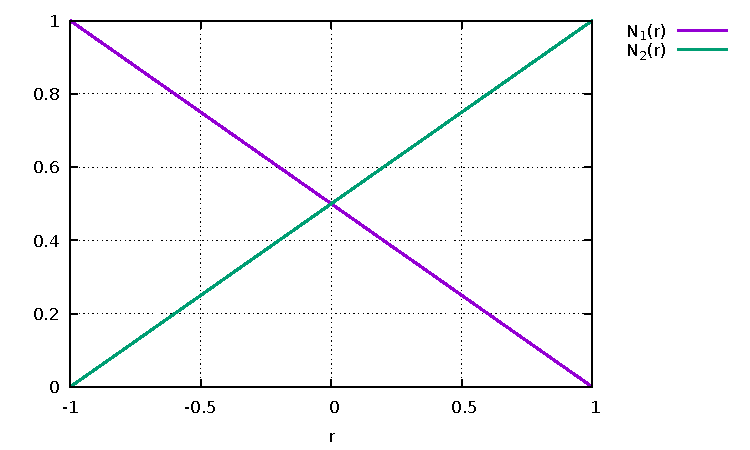
\includegraphics[width=8cm]{images/basis1D/linear.pdf}\\
{\captionfont Plot of the two linear functions $N_1(r)$ and $N_2(r)$.}
\end{center}

\newpage
%------------------------------------------
\subsubsection{Quadratic basis functions ($Q_2$) \label{sec:bf2}}
\index{general}{$Q_2$}

Let $f(r)$ be a $C^1$ function on the interval $[-1:1]$ with $f(-1)=f_1$, $f(0)=f_2$ and $f(1)=f_3$.
\begin{center}
\includegraphics[width=8cm]{images/quadshapefct.png}
\end{center}
Let us assume that the function $f(r)$ is to be approximated on $[-1,1]$ by the second order polynomial 
$f^h(r)$:
\begin{equation}
f(r)=a+br+cr^2 \label{eqquad}
\end{equation}
Then it must fulfil
\begin{eqnarray}
f^h(r=-1)&=&a-b+c = f_1 \nonumber\\
f^h(r=0) &=&a\quad\quad\quad\;     = f_2 \nonumber\\
f^h(r=+1)&=&a+b+c = f_3 \nonumber
\end{eqnarray}
This leads to
\begin{eqnarray}
a&=&f_2   \nn\\
b&=&\frac{1}{2}(-f_1+f_3)  \nn\\
c&=&\frac{1}{2}(f_1+f_3-2f_2) 
\end{eqnarray}
and then replacing $a,b,c$ in Eq.~\eqref{eqquad} by the above values on gets
\[
f^h(r)=\left[\frac{1}{2}r(r-1)\right] f_1 + (1-r^2) f_2 + \left[\frac{1}{2}r(r+1)\right] f_3
\]
or,
\[
\boxed{
f^h(r) = \sum_{i=1}^3 N_i(r) f_i
}
\]
with
\begin{mdframed}[backgroundcolor=blue!5]
\begin{eqnarray}
N_1(r) &=& \frac{1}{2}r(r-1) \nonumber\\
N_2(r) &=& (1-r^2) \nonumber\\ 
N_3(r) &=& \frac{1}{2}r(r+1) 
\end{eqnarray}
\end{mdframed}

\begin{center}
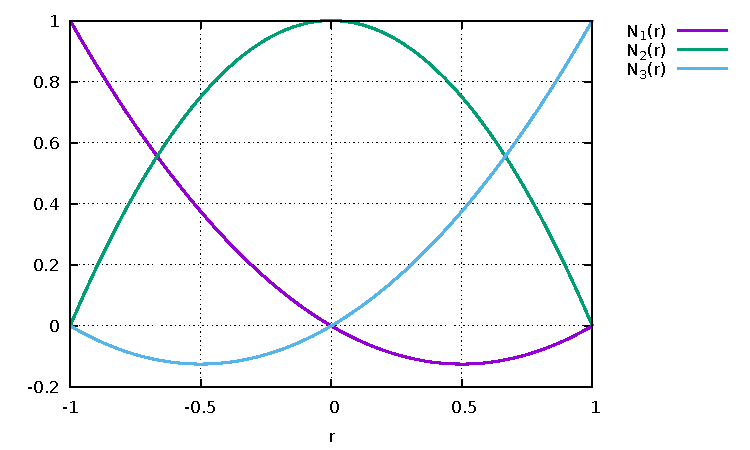
\includegraphics[width=8cm]{images/basis1D/quadratic.pdf}\\
{\captionfont Plot of the three quadratic functions $N_1(r)$, $N_2(r)$ and $N_3(r)$.}
\end{center}
Note that $Q_2$ basis functions can take negative values. 

We will later need the first-order derivatives of these functions:
\begin{mdframed}[backgroundcolor=blue!5]
\begin{eqnarray}
\frac{\partial N_1}{\partial r} &=& r-\frac{1}{2} \nonumber\\
\frac{\partial N_2}{\partial r} &=& -2r \nonumber\\ 
\frac{\partial N_3}{\partial r} &=& r+\frac{1}{2}
\end{eqnarray}
\end{mdframed}


%------------------------------------------
\subsubsection{Cubic basis functions ($Q_3$) \label{sec:bf3}}
\index{general}{$Q_3$}

We proceed as previously by assuming that the third-order 
polynomial representation of function $f(r)$ is given by
\[
f^h(r)=a+br+cr^2+dr^3
\]
with the nodes at position -1,-1/3, +1/3 and +1.
It then must fulfil all four conditions:
\begin{eqnarray}
f(-1)   &=& a-b+c-d = f_1 \nonumber\\
f(-1/3) &=& a-\frac{b}{3}+\frac{c}{9}-\frac{d}{27} = f_2 \nonumber\\
f(+1/3) &=& a-\frac{b}{3}+\frac{c}{9}-\frac{d}{27} = f_3 \nonumber\\
f(+1)   &=& a+b+c+d = f_4 \nonumber
\end{eqnarray}
Adding the first and fourth equation and the second and third, one arrives at
\[
f_1+f_4 = 2a+2c \quad\quad\quad f_2+f_3=2a+\frac{2c}{9}
\]
and finally:
\[
a=\frac{1}{16} \left( -f_1 + 9f_2 + 9f_3 - f_4  \right)
\]
\[
c=\frac{9}{16}\left(f_1-f_2-f_3+f_4\right)
\]
Combining the original 4 equations in a different way yields
\[
2b+2d=f_4-f_1 
\quad\quad\quad
\frac{2b}{3} + \frac{2d}{27} = f_3-f_2
\]
so that
\[
b=\frac{1}{16} \left( f_1 - 27f_2 + 27f_3 -f_4   \right)
\]
\[
d=\frac{9}{16} \left( -f_1 + 3f_2 - 3f_3 + f_4 \right)
\]
Finally,
\begin{eqnarray}
f^h(r) 
&=& a+b+cr^2+dr^3 \nonumber\\
&=& \frac{1}{16} (-1+  r +9r^2 - 9r^3 )f_1 \nonumber\\ 
&+& \frac{1}{16} ( 9-27r -9r^2 +27r^3 )f_2 \nonumber\\ 
&+& \frac{1}{16} ( 9+27r -9r^2 -27r^3 )f_3 \nonumber\\ 
&+& \frac{1}{16} (-1-  r +9r^2 + 9r^3 )f_4 \nonumber\\ 
&=& \sum_{i=1}^4 N_i(r) f_i \nonumber
\end{eqnarray}
where (see also for example \cite[p49]{li06})
\begin{mdframed}[backgroundcolor=blue!5]
\begin{eqnarray}
N_1&=& \frac{1}{16} (-1+  r+9r^2- 9r^3 ) \nonumber\\ 
N_2&=& \frac{1}{16} ( 9-27r-9r^2+27r^3 ) \nonumber\\ 
N_3&=& \frac{1}{16} ( 9+27r-9r^2-27r^3 ) \nonumber\\ 
N_4&=& \frac{1}{16} (-1-  r+9r^2+ 9r^3 ) \nonumber
\end{eqnarray}
\end{mdframed}

\begin{center}
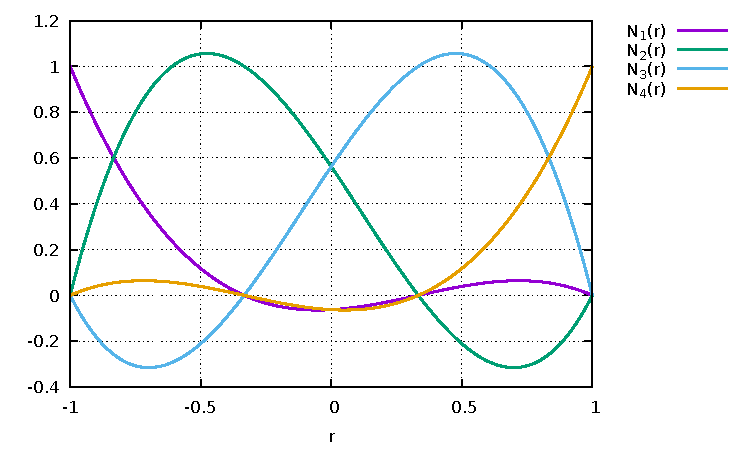
\includegraphics[width=8cm]{images/basis1D/cubic.pdf}\\
{\captionfont Plot of the four cubic functions $N_1(r)$, $N_2(r)$, $N_3(r)$ and $N_4(r)$.}
\end{center}

Let us now verify that these functions can represent any polynomial function up to third order:

\begin{itemize}
\item
Let us assume $f(r)=C$, then
\[
f^h(r) = \sum N_i(r) f_i = \sum_i N_i C = C \sum_i N_i  = C
\]
so that a constant function is exactly reproduced, as expected.
This is a very important property of the $N_i$ functions: They must fulfil $\sum\limits_i N_i =1$.

\item
Let us assume $f(r)= r$, then $f_1=-1$, $f_2=-1/3$, $f_3=1/3$ and $f_4=+1$. We then have
\begin{eqnarray}
f^h(r) 
&=& \sum N_i(r) f_i  \nonumber\\
&=& - N_1(r) -\frac{1}{3}N_2(r) + \frac{1}{3}N_3(r)  + N_4(r) \nonumber\\
&=& [-(-1+  r+9r^2- 9r^3 ) \nn\\
&&- \frac{1}{3} ( 9-27r-9r^2-27r^3 ) \nn\\
&&+ \frac{1}{3} ( 9+27r-9r^2+27r^3 ) \nn\\
&&+ (-1-  r+9r^2+ 9r^3 )]/16 \nonumber\\
&=& [-r +9r + 9r -r]/16  + ... 0 ... \nonumber\\
&=& r   
\end{eqnarray}

\item The cases $f(r)=r^2$ and $f(r)=r^3$ are left as exercise.

\end{itemize}

The basis functions first-order derivatives are given by
\begin{mdframed}[backgroundcolor=blue!5]
\begin{eqnarray}
\frac{\partial N_1}{\partial r}&=& \frac{1}{16}  (  1 +18r - 27r^2 ) \nonumber\\ 
\frac{\partial N_2}{\partial r}&=& \frac{1}{16}  (-27 -18r + 81r^2 ) \nonumber\\ 
\frac{\partial N_3}{\partial r}&=& \frac{1}{16}  (+27 -18r - 81r^2 ) \nonumber\\ 
\frac{\partial N_4}{\partial r}&=& \frac{1}{16}  ( -1 +18r + 27r^2 ) \nonumber
\end{eqnarray}
\end{mdframed}

We can also verify that the derivatives are also properly approximated:

\begin{itemize}
\item
Let us assume $f(r)=C$, then
\begin{eqnarray}
\frac{\partial f^h}{\partial r} 
&=& \sum_i \frac{\partial N_i}{\partial r} f_i  \nonumber\\
&=&  C \sum_i \frac{\partial N_i}{\partial r}  \nonumber\\
&=& \frac{C}{16} [  (  1 +18r - 27r^2 ) 
+ (-27 -18r + 81r^2 )  
+  (+27 -18r - 81r^2 ) 
+ ( -1 +18r + 27r^2 ) ]  \nonumber\\
&=& 0 \nonumber
\end{eqnarray}

\item
Let us assume $f(r)= r$, then $f_1=-1$, $f_2=-1/3$, $f_3=1/3$ and $f_4=+1$. We then have
\begin{eqnarray}
\frac{\partial f^h}{\partial r} 
&=& \sum_i \frac{\partial N_i}{\partial r} f_i  \nonumber\\
&=& \frac{1}{16} [  -(  1 +18r - 27r^2 ) 
 -\frac{1}{3} (-27 -18r + 81r^2 )  
 +\frac{1}{3} (27 -18r - 81r^2 )
 + ( -1 +18r + 27r^2 ) ]  \nonumber\\
&=& \frac{1}{16} [-2 + 18 + 54r^2 - 54r^2] \nonumber\\
&=& 1 \nonumber
\end{eqnarray}

\item
Let us assume $f(r)= r^2$, then $f_1=1$, $f_2=1/9$, $f_3=1/9$ and $f_4=1$. We then have
\begin{eqnarray}
\frac{\partial f^h}{\partial r} 
&=& \sum_i \frac{\partial N_i}{\partial r} f_i  \nonumber\\
&=& \frac{1}{16} \left[  
(  1 +18r - 27r^2 ) 
+\frac19 (-27 -18r + 81r^2 )  
+\frac19  (27 -18r - 81r^2 )
+ ( -1 +18r + 27r^2 ) \right]  \nonumber\\
&=& \frac{1}{16}(32r) \nn\\
&=& 2r
\end{eqnarray}
as expected.




\end{itemize}

%---------------------------------------------------------------
\subsubsection{Quartic basis functions ($Q_4$) \label{sec:bf4}}
\index{general}{$Q_4$}

The 1D basis polynomial is given by
\[
f_h(r)=a+br+cr^2+dr^3+er^4
\]
with the nodes at position -1,-1/2, 0, +1/2 and +1.
The function $f^h(r)$ must then fulfil 
\begin{eqnarray}
f_h(-1)   &=& a-b+c-d+e = f_1 \nonumber\\
f_h(-1/2) &=& a-\frac{b}{2}+\frac{c}{4}-\frac{d}{8}+\frac{e}{16} = f_2 \nonumber\\
f_h(0)    &=& a = f_3 \nonumber\\
f_h(+1/2) &=& a-\frac{b}{2}+\frac{c}{4}-\frac{d}{8}+\frac{e}{16} = f_4 \nonumber\\
f_h(+1)   &=& a+b+c+d+e = f_5 \nonumber
\end{eqnarray}
or, 
\begin{equation}
\left(
\begin{array}{ccccc}
 1  &  -1  &  1 &  -1 &  1 \\ 
 1  &  -1/2  &  1/4 &  -1/8 &  1/16 \\ 
 1  &   0    &  0   &   0   & 0 \\
 1  &  1/2  &  1/4 &  1/8 &  1/16 \\ 
 1  &  1  &  1 &  1 &  1 
\end{array}
\right)
\left(
\begin{array}{c}
a \\ b \\ c \\ d \\ e
\end{array}
\right)
=
\left(
\begin{array}{c}
f_1 \\ f_2 \\ f_3 \\ f_4 \\ f_5
\end{array}
\right)
\end{equation}
The third line gives $a=f_3$ so that
\begin{equation}
\underbrace{
\left(
\begin{array}{ccccc}
-1  &  1   &  -1 &  1 \\ 
-1/2 &  1/4 & -1/8 &  1/16 \\ 
 1/2 &  1/4 &  1/8 &  1/16 \\ 
 1  &  1   &  1 &  1 
\end{array}
\right)}_{A}
\left(
\begin{array}{c}
b \\ c  \\ d \\ e
\end{array}
\right)
=
\left(
\begin{array}{c}
f_1 -f_3 \\ f_2 -f_3\\ f_4-f_3 \\ f_5 -f_3
\end{array}
\right)
\end{equation}
The inverse of the matrix $A$ is:
\[
A^{-1}=
\frac{1}{6}
\left(
\begin{array}{ccccc}
1 & -8 & 8 & -1 \\
-1 & 16 & 16 & -1 \\
-4 & 8 & -8 & 4 \\
4 & -16 & -16 & 4
\end{array}
\right)
\]
so that 
\[
\left(
\begin{array}{c}
b \\ c \\ d \\ e
\end{array}
\right)
=
\frac{1}{6}
\left(
\begin{array}{ccccc}
1 & -8 & 8 & -1 \\
-1 & 16 & 16 & -1 \\
-4 & 8 & -8 & 4 \\
4 & -16 & -16 & 4
\end{array}
\right)
\cdot
\left(
\begin{array}{c}
f_1 -f_3 \\ f_2 -f_3\\ f_4-f_3 \\ f_5 -f_3
\end{array}
\right)
\]
and then 
\begin{eqnarray}
b &=& \frac{1}{6} \left( f_1 -8f_2 +8 f_4 -f_5     \right) \\
c &=& \frac{1}{6} \left( -f_1 +16f_2 -30f_3    + 16f_4- f_5   \right) \\
d &=& \frac{1}{6} \left( -4f_1 +8f_2     -8f_4+ 4 f_5   \right) \\
e &=& \frac{1}{6} \left( 4f_1 -16f_2 +24f_3 -16f_4+ 4 f_5   \right) 
\end{eqnarray}
Finally
\begin{eqnarray}
f_h(r) 
&=& a+br+cr^2+dr^3+er^4 \nn\\
&=& f_3 + 
\frac{1}{6} \left( f_1 -8f_2 +8 f_4 -f_5     \right)  r  +
\frac{1}{6} \left( -f_1 +16f_2 -30f_3    + 16f_4- f_5   \right) r^2 + \nn\\ &&
\frac{1}{6} \left( -4f_1 +8f_2     -8f_4+ 4 f_5   \right) r^3 +
\frac{1}{6} \left( 4f_1 -16f_2 +24f_3 -16f_4+ 4 f_5   \right) r^4 \nn\\
&=& \frac{1}{6} \left(  r- r^2 -4r^3 +4r^4\right) f_1 \nn\\
&+& \frac{1}{6} \left(  -8r+16 r^2 +8r^3 -16 r^4\right) f_2 \nn\\
&+& \left( 1 -5r^2+4r^4  \right) f_3 \nn\\
&+& \frac{1}{6} \left(  8r+16 r^2 -8r^3 -16 r^4\right) f_4 \nn\\
&+& \frac{1}{6} \left(  -r- r^2 +4r^3 +4r^4\right) f_5 \nn
\end{eqnarray}
with 
\begin{mdframed}[backgroundcolor=blue!5]
\begin{eqnarray}
N_1(r)&=& \frac{1}{6} \left(  r- r^2 -4r^3 +4r^4\right) \nn\\
N_2(r)&=& \frac{1}{6} \left(  -8r+16 r^2 +8r^3 -16 r^4\right)  \nn\\
N_3(r)&=& \left( 1 -5r^2+4r^4  \right) \nn \\
N_4(r)&=& \frac{1}{6} \left(  8r+16 r^2 -8r^3 -16 r^4\right)  \nn\\
N_5(r)&=& \frac{1}{6} \left(  -r- r^2 +4r^3 +4r^4\right) 
\end{eqnarray}
\end{mdframed}

\begin{center}
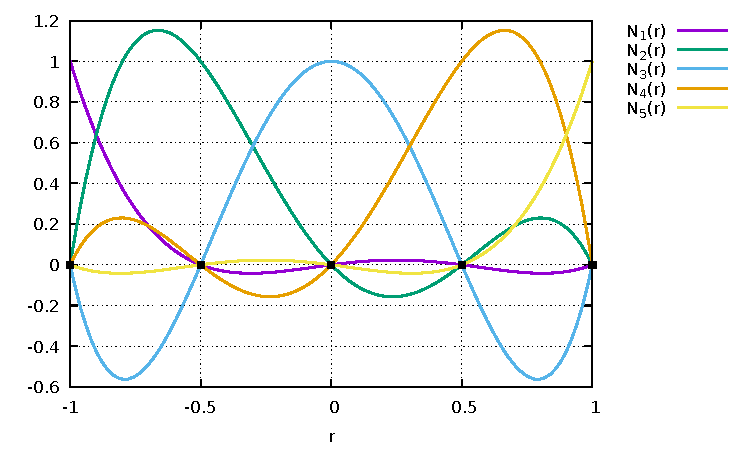
\includegraphics[width=8cm]{images/basis1D/quartic.pdf}\\
{\captionfont Plot of the 5 quartic basis functions.}
\end{center}

The basis functions derivative are given by
\begin{mdframed}[backgroundcolor=blue!5]
\begin{eqnarray}
\frac{\partial N_1}{\partial r}&=& \frac{1}{6}(1-2r-12r^2+16r^3) \nn\\
\frac{\partial N_2}{\partial r}&=& \frac{1}{6}(-8+32r+24r^2-64r^3) \nn\\
\frac{\partial N_3}{\partial r}&=& -10r+16r^3 \nn\\
\frac{\partial N_4}{\partial r}&=& \frac{1}{6} (8+32r-24r^2-64r^3) \nn\\
\frac{\partial N_5}{\partial r}&=& \frac{1}{6} (-1-2r+12r^2+16r^3) 
\end{eqnarray}
\end{mdframed}


%---------------------------------------------------------------
\subsubsection{Quartic basis functions ($Q_6$) \label{sec:bf6}}
\index{general}{$Q_6$}

The 1D basis polynomial is given by
\[
f_h(r)=a+br+cr^2+dr^3+er^4+fr^5+gr^6
\]
with the nodes at position -1,-2/3, -1/3, 0, +1/3, +2/3 and +1.
The function $f^h(r)$ must then fulfil 
%\begin{eqnarray}
%f_h(-1)   &=&  a -        b +         c -            d +e -f +g =f_1 \nn\\
%f_h(-2/3) &=&  a -\frac23 b + \frac49 c -\frac{8}{27}d +e -f +g =f_2\nn\\
%f_h(-1/3) &=&  a -\frac13 b + \frac19 c -\frac{1}{27}d +e -f +g =f_3\nn\\
%f_h(0)    &=&  a                                                = f_4 \nn\\
%f_h(+1/3) &=&  a +\frac13 b + \frac19 c +\frac{1}{27}d +e +f +g =f_5\nn\\
%f_h(+2/3) &=&  a +\frac23 b + \frac49 c +\frac{8}{27}d +e +f =g =f_6\nn\\
%f_h(+1)   &=&  a +        b +         c +            d +e +f +g =f_7 \nn
%\end{eqnarray}


\[
\left(
\begin{array}{ccccccc}
1& -1       & 1       & -1           & 1 & -1 & 1  \\
1& -\frac23 & \frac49 & -\frac{8}{27}& \frac{16}{81} & -\frac{32}{243} & \frac{64}{729}  \\
1& -\frac13 & \frac19 & -\frac{1}{27}& \frac{1}{81}  & -\frac{1}{243}  & \frac{1}{729}  \\
1& 0        & 0       & 0            &0 & 0 & 0 \\
1& \frac13  & \frac19 & \frac{1}{27} & \frac{1}{81}  & \frac{1}{243}  & \frac{1}{729}  \\
1& \frac23  & \frac49 & \frac{8}{27} & \frac{16}{81} & \frac{32}{243} & \frac{64}{729}  \\
1& 1        & 1       & 1            & 1 & 1 & 1  
\end{array}
\right)
\cdot
\left(
\begin{array}{c}
a \\ b \\ c \\ d \\ e \\ f \\ g
\end{array}
\right)
=
\left(
\begin{array}{c}
f_1 \\ f_2 \\ f_3 \\ f_4 \\ f_5 \\ f_6 \\ f_7
\end{array}
\right)
\]


The middle line yields $a=f_4$, so that we have:

\[
\left(
\begin{array}{cccccc}
 -1       & 1       & -1           & 1 & -1 & 1  \\
 -\frac23 & \frac49 & -\frac{8}{27}& \frac{16}{81} & -\frac{32}{243} & \frac{64}{729}  \\
 -\frac13 & \frac19 & -\frac{1}{27}& \frac{1}{81}  & -\frac{1}{243}  & \frac{1}{729}  \\
 \frac13  & \frac19 & \frac{1}{27} & \frac{1}{81}  & \frac{1}{243}  & \frac{1}{729}  \\
 \frac23  & \frac49 & \frac{8}{27} & \frac{16}{81} & \frac{32}{243} & \frac{64}{729}  \\
 1        & 1       & 1            & 1 & 1 & 1  
\end{array}
\right)
\cdot
\left(
\begin{array}{c}
b \\ c \\ d \\ e \\ f \\ g
\end{array}
\right)
=
\left(
\begin{array}{c}
f_1 -f_4 \\ f_2 -f_4\\ f_3 -f_4 \\ f_5 -f_4\\ f_6 -f_4\\ f_7-f_4
\end{array}
\right)
\]
Multiplying all lines by 729, we obtain:

\[
\frac{1}{729}
\left(
\begin{array}{cccccc}
 -729 & 729 & -729 & 729 & -729 & 729  \\
 -486 & 324 & -216 & 144 & -96  & 64  \\
 -243 & 81  & -27  & 9   & -3   & 1  \\
 243  & 81  & 27   & 9   & 3    & 1  \\
 486  & 324 & 216  & 144 & 96   & 64  \\
729   & 729 & 729  & 729 & 729  & 729  
\end{array}
\right)
\cdot
\left(
\begin{array}{c}
b \\ c \\ d \\ e \\ f \\ g
\end{array}
\right)
=
\left(
\begin{array}{c}
f_1 -f_4 \\ f_2 -f_4\\ f_3 -f_4 \\ f_5 -f_4\\ f_6 -f_4\\ f_7-f_4
\end{array}
\right)
\]

The inverse\footnote{\url{https://physandmathsolutions.com/Matrices/matrix_inverse/matrix_inverse_6x6.php}} of this matrix is:

\begin{verbatim}
-0.00006859 	0.00061728 	-0.00308642 	0.00308642 	-0.00061728 	0.00006859
0.00006859 	-0.00092593 	0.00925926 	0.00925926 	-0.00092593 	0.00006859
0.00077160 	-0.00617284 	0.01003086 	-0.01003086 	0.00617284 	-0.00077160
-0.00077160 	0.00925926 	-0.03009259 	-0.03009259 	0.00925926 	-0.00077160
-0.00138889 	0.00555556 	-0.00694444 	0.00694444 	-0.00555556 	0.00138889
0.00138889 	-0.00833333 	0.02083333 	0.02083333 	-0.00833333 	0.00138889
\end{verbatim}

Obviously, this is not a very practical approach anymore. One could 
solve the system by hand, making sure to keep fractions but it will be 
cumbersome. Let us turn to another approach.

The nodes inside the reference element are as follows:

\begin{verbatim}
(1) (2)  (3) (4) (5)  (6) (7)
-|---|----|---+---|----|---|-
-1 -2/3 -1/3  0  1/3  2/3  1
\end{verbatim}

Basis function $\bN_1(r)$ is a 6th order polynomial expression 
that should be 1 at node 1, and 0 at others,
i.e. at $r=-2/3,-1/3,0,1/3,2/3,1$. It must then be of the form:
\[
\bN_1(r) = \alpha(r+\frac23)(r+\frac13)(r)(r-\frac13)(r-\frac23)(r-1)
\]
When evaluated at $r=-1$, we get
\[
\bN_1(r=-1) 
= \alpha(-\frac13)(-\frac23)(-1)(-\frac43)(-\frac53)(-2)
= \alpha\frac{80}{81}
\]
Since this quantity must be 1, we have
\[
1 = \alpha \frac{80}{81}
\quad
\rightarrow
\quad
\alpha=\frac{81}{80}
\]
so that 
\begin{eqnarray}
\bN_1(r)
&=& \frac{81}{80}(r+\frac23)(r+\frac13)(r)(r-\frac13)(r-\frac23)(r-1) \nn\\
&=& \frac{81}{80} \frac{1}{81} (3r+2)(3r+1)(r)(3r-1)(3r-2)(r-1) \nn\\
&=& \frac{1}{80} (9r^2-4)(9r^2-1)(r^2-r) \nn\\
&=& \frac{1}{80} (81r^4 -45r^2 +4)(r^2-r) 
\end{eqnarray}

Moving to $\bN_2(r)$, we have
\[
\bN_2(r)= \alpha(r+1)(r+\frac13)(r)(r-\frac13)(r-\frac23)(r-1)
\]
which must be equal to 1 for $r=-2/3$:
\begin{eqnarray}
\bN_2(r=-2/3)
&=& \alpha(-\frac23+1)(-\frac23+\frac13)(-\frac23)(-\frac23-\frac13)(-\frac23-\frac23)(-\frac23-1)\nn\\
&=& \alpha (\frac13)(-\frac13)(-\frac23)(-1)(-\frac43)(-\frac53)\nn\\
&=& -\alpha \frac{40}{243}
\end{eqnarray}
so that 
\[
\bN_2(r)= -\frac{243}{40}(r+1)(r+\frac13)(r)(r-\frac13)(r-\frac23)(r-1)
\]

Moving to $\bN_3(r)$, we have
\[
\bN_3(r)= \alpha(r+1)(r+\frac23)(r)(r-\frac13)(r-\frac23)(r-1)
\]
which must be equal to 1 for $r=-1/3$:
\begin{eqnarray}
\bN_3(r=-1/3)
&=& \alpha(-\frac13+1)(-\frac13+\frac23)(-\frac13)(-\frac13-\frac13)(-\frac13-\frac23)(-\frac13-1) \nn\\
&=& \alpha(\frac23)(\frac13)(-\frac13)(-\frac23)(-1)(-\frac43) \nn\\
&=& \alpha \frac{16}{243}
\end{eqnarray}
so that 
\[
\bN_3(r)= \frac{243}{16}(r+1)(r+\frac23)(r)(r-\frac13)(r-\frac23)(r-1)
\]
Likewise, we arrive at the rest of the basis functions. In the end:

\begin{eqnarray}
\bN_1(r) &=& \frac{81}{80}(r+\frac23)(r+\frac13)(r)(r-\frac13)(r-\frac23)(r-1) \nn\\
\bN_2(r) &=& -\frac{243}{40}(r+1)(r+\frac13)(r)(r-\frac13)(r-\frac23)(r-1) \nn\\
\bN_3(r) &=& \frac{243}{16}(r+1)(r+\frac23)(r)(r-\frac13)(r-\frac23)(r-1) \nn\\
\bN_4(r) &=& -\frac{81}{4}(r+1)(r+\frac23)(r+\frac13)(r-\frac13)(r-\frac23)(r-1) \nn\\
\bN_5(r) &=& \frac{243}{16}(r+1)(r+\frac23)(r+\frac13)(r)(r-\frac23)(r-1) \nn\\
\bN_6(r) &=& -\frac{243}{40}(r+1)(r+\frac23)(r+\frac13)(r)(r-\frac13)(r-1) \nn\\
\bN_7(r) &=& \frac{81}{80}(r+1)(r+\frac23)(r+\frac13)(r)(r-\frac13)(r-\frac23)
\end{eqnarray}
or 

\begin{mdframed}[backgroundcolor=blue!5]
\begin{eqnarray}
\bN_1(r) &=& \frac{1}{80}(81r^6-81r^5-45r^4+45r^3+4r^2-4r) \nn\\
\bN_2(r) &=& -\frac{9}{40}(27r^6 -18r^5 -30r^4 +20r^3 +3r^2 -2r) \nn\\ 
\bN_3(r) &=& \frac{9}{16} (27r^6 -9r^5 -39r^4 +13r^3 +12r^2 -4r) \nn\\ 
\bN_4(r) &=& -\frac{1}{4} (81r^6 - 126r^4+49r^2 +4) \nn\\ 
\bN_5(r) &=& \frac{9}{16} (27r^6 +9r^5 -39r^4 -13r^3 +12r^2 +4r) \nn\\ 
\bN_6(r) &=& -\frac{9}{40}(27r^6 +18r^5 -30r^4 -20r^3 +3r^2 +2r) \nn\\ 
\bN_7(r) &=&  \frac{1}{80}(81r^6+81r^5-45r^4-45r^3+4r^2+4r) 
\end{eqnarray}
\end{mdframed}

\begin{center}
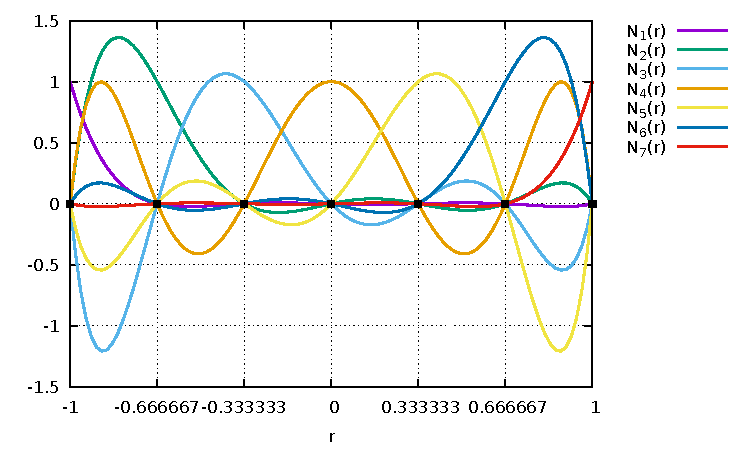
\includegraphics[width=11cm]{images/basis1D/Q6.pdf}\\
{\captionfont Plot of the 7 six-order basis functions.}
\end{center}

Using WolframAlpha\footnote{\url{https://www.wolframalpha.com/}}, we arrive at 

\begin{eqnarray}
\frac{d \bN_1}{dr} &=& \frac{1}{80} (486r^5 - 405r^4 - 180r^3 + 135 r^2 +8r-4) \nn\\
\frac{d \bN_2}{dr} &=& -\frac{9}{20} (81r^5 - 45r^4 -60r^3 + 30r^2 +3r -1) \nn\\ 
\frac{d \bN_3}{dr} &=& \frac{9}{16} (162r^5-45r^4 -156r^3 +39r^2 +24r -4) \nn\\ 
\frac{d \bN_4}{dr} &=& \frac{1}{2} (-243r^5+252r^3-49r) \nn\\
\frac{d \bN_5}{dr} &=& \frac{9}{16} (162r^5 +45r^4 -156r^3 -39r^2 +24r +4) \nn\\ 
\frac{d \bN_6}{dr} &=& -\frac{9}{20} (81r^5 +45r^4 -60r^3 - 30r^2 +3r +1) \nn\\ 
\frac{d \bN_7}{dr} &=& \frac{1}{80} (486r^5 + 405r^4 - 180r^3 -135r^2 +8r+4) 
\end{eqnarray}









 %-------------
\newpage
\section{Elements and basis functions in 2D}\label{sec:shpfct2d} \begin{flushright} {\tiny {\color{gray} elements2D.tex}} \end{flushright}
%~~~~~~~~~~~~~~~~~~~~~~~~~~~~~~~~~~~~~~~~~~~~~~~~~~~~~~~~~~~~~~~~~~~~~~~~~~~~~~~~~~~~~~~~~~~~~~~~~~

Let us for a moment consider a single quadrilateral element in the $xy$-plane, 
as shown on the following figure:
\begin{center}
\includegraphics[width=5.8cm]{images/shape}
\end{center}
Let us assume that we know the values of a given field $u$ at the four vertices.
For a given point $M$ inside the element in the plane, what is the value of the 
field $u$ at this point?
It makes sense to postulate that $u_M$ will be given  by 
\[
u_M= \phi(u_1,u_2,u_3,u_4,x_M,y_M) 
\]
where $\phi$ is a function to be determined. Although $\phi$ is not unique, we can 
decide to express the value $u_M$ as a weighed sum of the values at the vertices $u_i$.
One option could be to assign all four vertices the same weight, say $1/4$ so that 
$u_M=(u_1+u_2+u_3+u_4)/4$, i.e. $u_M$ is simply given by the arithmetic mean 
of the vertices values. 
If the function $u(x,y)$ is such that it is a constant function, say $u(x,y)=C$, 
then $u_M=(u_1+u_2+u_3+u_4)/4=(C+C+C+C)/4=C$ and the result is exact.
However, for any other function $u$ the value $u_M$ will not be as accurate.
Also, this approach suffers from a major drawback as it does
not use the location of point $M$ inside the element. For instance, when 
$(x_M,y_M) \rightarrow (x_2,y_2)$ we expect $u_M \rightarrow u_2$ but $u_M$ would 
remain equal to $(u_1+u_2+u_3+u_4)/4$.

In light of this, we could now assume that the weights would depend on the position 
of $M$ in a continuous fashion:
\begin{equation}
u(x_M,y_M) = \sum_{i=1}^4 \bN_i(x_M,y_M)\;  u_i
= \bN_1(x_M,y_M) u_1 + \bN_2(x_M,y_M) u_2 + \bN_3(x_M,y_M) u_3 + \bN_4(x_M,y_M) u_4 
\end{equation}
where the $bN_i$ are continuous (and also "well behaved") functions which have the property:
\[
\bN_i(x_j,y_j)=\delta_{ij}
\]
or, in other words for example: 
\begin{eqnarray}
\bN_3(x_1,y_1) &=& 0 \nn\\
\bN_3(x_2,y_2) &=& 0 \nn\\
\bN_3(x_3,y_3) &=& 1 \nn\\
\bN_3(x_4,y_4) &=& 0 
\end{eqnarray}
The functions $\bN_i$ are commonly called basis functions. \index{general}{basis functions}

Omitting the $M$ subscripts (yet stil assuming the point being inside the element), the velocity 
components $u$ and $v$ for a point inside the element
 are given by:
\begin{eqnarray}
u^h(x,y) &=& \sum_{i=1}^4 \bN_i(x,y)\;  u_i \\
v^h(x,y) &=& \sum_{i=1}^4 \bN_i(x,y)\;  v_i \label{bf01}
\end{eqnarray}
where we have added the superscript $h$ to denote that it is an approximation of the functions 
of this element of diameter $h$ (by diameter we mean here a representative scalar value of the dimension
of the element). 

One can now easily compute velocity gradients (and therefore the 
strain rate tensor) since we have assumed the basis functions to be "well behaved" 
(in this case first-order differentiable):
\begin{eqnarray}
\dot{\varepsilon}^h_{xx}(x,y) 
&=& \frac{\partial u^h}{\partial x} = \sum_{i=1}^4 \frac{\partial \bN_i}{\partial x}\;  u_i \\
\dot{\varepsilon}^h_{yy}(x,y) 
&=& \frac{\partial v^h}{\partial y} = \sum_{i=1}^4 \frac{\partial \bN_i}{\partial y}\;  v_i \\
\dot{\varepsilon}^h_{xy}(x,y) 
&=& \frac{1}{2}\left(\frac{\partial u^h}{\partial y} + \frac{\partial v^h}{\partial x} \right) 
= \frac{1}{2}\sum_{i=1}^4 \frac{\partial \bN_i}{\partial y}\;  u_i
+ \frac{1}{2}\sum_{i=1}^4 \frac{\partial \bN_i}{\partial x}\;  v_i
\end{eqnarray}
How we actually obtain the exact form of the basis functions $\bN_i$ is explained in the coming sections.

%%%%%%%%%%%%%%%%%%%%%%%%%%%%%%%%%%%%%%%%%%%%%%%%%%%%%%%%%%%%%%%%%%%%%%%%%%%%%%%
\subsection{Bilinear basis functions in 2D ($Q_1$)} \label{ss:q12d}
\index{general}{$Q_1$}

\begin{flushright} {\tiny {\color{gray} basis\_Q1\_2D.tex}} \end{flushright}
%~~~~~~~~~~~~~~~~~~~~~~~~~~~~~~~~~~~~~~~~~~~~~~~~~~~~~~~~~~~~~~~~~~~~~~~~~~~~~~~~~~~~~~~~~~~~~~~~~~

In this section, we consider for simplicity an element which is a square defined 
by $-1<r<1$, $-1<s<1$ in the Cartesian coordinates system $(r,s)$\footnote{There is a 
reason to choose $r$ and $s$ as coordinates and not $x$ and $y$ as we will see later.}:

\input{tikz/tikz_q12d}

Note the counter-clockwise numbering\footnote{Note that in many of the python codes which 
are part of this project the numbering starts at 0.}.
This element is commonly called the reference element. How we go from the $(x,y)$ coordinate system 
to the $(r,s)$ once and vice versa will be dealt with later on.
The basis functions in the above reference element in the reduced 
coordinates system $(r,s)$ are given by:
\begin{mdframed}[backgroundcolor=blue!5]
\begin{eqnarray}
\bN_1(r,s)&=&0.25(1-r)(1-s) \nonumber\\
\bN_2(r,s)&=&0.25(1+r)(1-s) \nonumber\\
\bN_3(r,s)&=&0.25(1+r)(1+s) \nonumber\\
\bN_4(r,s)&=&0.25(1-r)(1+s) 
\end{eqnarray}
\end{mdframed}
These basis functions are the product of the linear basis functions of Section~\ref{sec:bf1}
in the $r$ direction and the $s$ direction.
\begin{center}
\includegraphics[width=4cm]{images/basis_Q1_2D/N1}
\includegraphics[width=4cm]{images/basis_Q1_2D/N2}
\includegraphics[width=4cm]{images/basis_Q1_2D/N3}
\includegraphics[width=4cm]{images/basis_Q1_2D/N4}\\
{\captionfont Surface representation of the basis functions on the reference element.
{\color{gray} in images/basis\_Q1\_2D/ }}
\end{center}
The partial derivatives of these functions with respect to $r$ ans $s$ automatically follow:
\begin{mdframed}[backgroundcolor=blue!5]
\begin{align}
\frac{\partial \bN_1}{\partial r}(r,s)&= - 0.25(1-s) &
\frac{\partial \bN_1}{\partial s}(r,s)&= - 0.25(1-r) \nonumber\\
\frac{\partial \bN_2}{\partial r}(r,s)&= + 0.25(1-s) &
\frac{\partial \bN_2}{\partial s}(r,s)&= - 0.25(1+r) \nonumber\\
\frac{\partial \bN_3}{\partial r}(r,s)&= + 0.25(1+s) &
\frac{\partial \bN_3}{\partial s}(r,s)&= + 0.25(1+r) \nonumber\\
\frac{\partial \bN_4}{\partial r}(r,s)&= - 0.25(1+s) &
\frac{\partial \bN_4}{\partial s}(r,s)&= + 0.25(1-r) \nonumber
\end{align}
\end{mdframed}
Let us go back to Eq.~\eqref{bf01} and let us assume that the 
function $v(r,s)=C$ so that $v_i=C$ for $i=1,2,3,4$. 
It then follows that 
\[
v^h(r,s) = \sum_{i=1}^4 \bN_i(r,s)\;  v_i 
=C \sum_{i=1}^4 \bN_i(r,s)
=C [
\bN_1(r,s)
+\bN_2(r,s)
+\bN_3(r,s)
+\bN_4(r,s)]=C
\]
This is a very important property: if the $v$ function used to 
assign values at the vertices is constant, then 
the value of $v^h$ {\it anywhere} in the element is exactly $C$.
If we now turn to the derivatives of $v$ with respect to $r$ and $s$:
\[
\frac{\partial {v}^h}{\partial r}(r,s) 
= \sum_{i=1}^4 \frac{\partial \bN_i}{\partial r}(r,s)\;  v_i 
= C \sum_{i=1}^4 \frac{\partial \bN_i}{\partial r}(r,s) 
= C \left[ - 0.25(1-s)  + 0.25(1-s)  + 0.25(1+s)  - 0.25(1+s) \right] = 0 
\]

\[
\frac{\partial v^h}{\partial s}(r,s) 
= \sum_{i=1}^4 \frac{\partial \bN_i}{\partial s}(r,s)\;  v_i 
= C \sum_{i=1}^4 \frac{\partial \bN_i}{\partial s}(r,s) 
= C \left[ - 0.25(1-r) - 0.25(1+r) + 0.25(1+r) + 0.25(1-r) \right] = 0 
\]
We reassuringly find that the derivative of a constant field anywhere in the element is exactly zero.

If we now choose $v(r,s)=ar+bs$ with $a$ and $b$ two constant scalars, we find:
\begin{eqnarray}
v^h(r,s) 
&=& \sum_{i=1}^4 \bN_i(r,s)\;  v_i  \nn\\
&=& \sum_{i=1}^4 \bN_i(r,s) (ar_i+bs_i) \nn\\
&=& a \sum_{i=1}^4 \bN_i(r,s) r_i + b \sum_{i=1}^4 \bN_i(r,s) s_i \nn\\
&=& a \left[ 
 \frac14(1-r)(1-s)(-1)
+\frac14(1+r)(1-s)(+1)
+\frac14(1+r)(1+s)(+1)
+\frac14(1-r)(1+s)(-1) \right]  \nonumber\\
&+& b  
\left[ 
 \frac14(1-r)(1-s)(-1)
+\frac14(1+r)(1-s)(-1)
+\frac14(1+r)(1+s)(+1)
+\frac14(1-r)(1+s)(+1) \right]  \nonumber\\
&=& \frac{a}{4} \left[ 
-(1-r)(1-s)
+(1+r)(1-s)
+(1+r)(1+s)
-(1-r)(1+s) \right]  \nonumber\\
&+& \frac{b}{4}
\left[ 
-(1-r)(1-s)
-(1+r)(1-s)
+(1+r)(1+s)
+(1-r)(1+s) 
\right]  \nonumber\\
&=& ar+bs
\end{eqnarray}
This set of bilinear basis functions is therefore capable of exactly representing a bilinear field.
The derivatives are:
\begin{eqnarray}
\frac{\partial v^h}{\partial r}(r,s) 
&=& \sum_{i=1}^4 \frac{\partial \bN_i}{\partial r}(r,s)\;  v_i  \nn\\
&=& a \sum_{i=1}^4 \frac{\partial \bN_i}{\partial r}(r,s) r_i 
+ b \sum_{i=1}^4 \frac{\partial \bN_i}{\partial r}(r,s) s_i \nn\\
&=& a \left[
- \frac14(1-s)(-1) 
+ \frac14(1-s)(+1) 
+ \frac14(1+s)(+1) 
- \frac14(1+s)(-1) 
\right] \nonumber\\
&+&b \left[
- \frac14(1-s)(-1) 
+ \frac14(1-s)(-1) 
+ \frac14(1+s)(+1) 
- \frac14(1+s)(+1) 
\right] \nonumber\\
&=& \frac{a}{4} \left[
 (1-s)
+ (1-s)
+ (1+s)
+ (1+s)
\right] \nonumber\\
&+&\frac{b}{4} \left[
 (1-s)
- (1-s)
+ (1+s)
- (1+s)
\right] \nonumber\\
&=& a 
\end{eqnarray}
Here again, we find that the derivative of the bilinear field inside the element is exact: 
$\frac{\partial v^h}{\partial r} = \frac{\partial v}{\partial r}$.

However, following the same methodology as above, one can easily prove 
that this is no more true for polynomials of degree strictly higher than 1. 
This fact has serious consequences: if the solution to the problem at hand is 
for instance a parabola, the $Q_1$ basis functions cannot represent the solution properly, 
but only by approximating the parabola in each element by a line. As we will see 
later, $Q_2$ basis functions can remedy this problem by containing quadratic terms.

\begin{remark}
The $Q_1$ basis functions are first-order polynomials. We have seen that they can be used to compute
gradients. However they cannot be used to compute 2nd-order derivatives since their 2nd-order
derivative is identically zero.
\end{remark}

An identical approach to arrive at the basis functions is presented in 
\textcite{eriz68} (1968).



%%%%%%%%%%%%%%%%%%%%%%%%%%%%%%%%%%%%%%%%%%%%%%%%%%%%%%%%%%%%%%%%%%%%%%%%%%%%%%%
\subsection{Biquadratic basis functions in 2D ($Q_2$)}\label{ss:q22d}
\index{general}{$Q_2$}

\begin{flushright} {\tiny {\color{gray} \tt basis\_Q2\_2D.tex}} \end{flushright}
%~~~~~~~~~~~~~~~~~~~~~~~~~~~~~~~~~~~~~~~~~~~~~~~~~~~~~~~~~~~~~~~~~~~~~~~~~~~~~~~~~~~~~~~~~~~~~~~~~~

This element is part of the so-called Lagrange family \cite{raki00}. 
Inside an element the local numbering of the nodes is as follows\footnote{I have adopted here 
a numbering scheme starting at zero! Also, it is a numbering among many other possible choices!}:

\input{tikz/tikz_q22d}

Note that this numbering is also employed in Li \cite[p56]{li06}.
The polynomial representation of the function $\phi$ over this element is then taken to be biquadratic:
\[
\phi^h(r,s) = a + br + cs + drs + er^2 + fs^2 + gr^2s + hrs^2 + i r^2s^2 = \sum_{i=0}^8 \bN_i(r,s) \phi_i
\]
and one can show that the basis functions are:
\begin{mdframed}[backgroundcolor=blue!5]
\begin{eqnarray}
\bN_0(r,s)&=& \frac{1}{2}r(r-1)  \frac{1}{2}s(s-1)\nonumber\\
\bN_1(r,s)&=& \frac{1}{2}r(r+1)  \frac{1}{2}s(s-1)\nonumber\\
\bN_2(r,s)&=& \frac{1}{2}r(r+1)  \frac{1}{2}s(s+1)\nonumber\\
\bN_3(r,s)&=& \frac{1}{2}r(r-1)  \frac{1}{2}s(s+1)\nonumber\\
\bN_4(r,s)&=&     (1-r^2)  \frac{1}{2}s(s-1)\nonumber\\
\bN_5(r,s)&=& \frac{1}{2}r(r+1)      (1-s^2)\nonumber\\
\bN_6(r,s)&=&     (1-r^2)  \frac{1}{2}s(s+1)\nonumber\\
\bN_7(r,s)&=& \frac{1}{2}r(r-1)      (1-s^2)\nonumber\\
\bN_8(r,s)&=&     (1-r^2)      (1-s^2)\nonumber
\end{eqnarray}
\end{mdframed}
Note that we have $\bN_i(r_j,s_j)=\delta_{ij}$ and then obviously $\bN_i(r_i,s_i)=1$. 

\begin{center}
\includegraphics[width=4cm]{images/basis_Q2_2D/N1}
\includegraphics[width=4cm]{images/basis_Q2_2D/N2}
\includegraphics[width=4cm]{images/basis_Q2_2D/N3}\\
\includegraphics[width=4cm]{images/basis_Q2_2D/N4}
\includegraphics[width=4cm]{images/basis_Q2_2D/N5}
\includegraphics[width=4cm]{images/basis_Q2_2D/N6}\\
\includegraphics[width=4cm]{images/basis_Q2_2D/N7}
\includegraphics[width=4cm]{images/basis_Q2_2D/N8}
\includegraphics[width=4cm]{images/basis_Q2_2D/N9}\\
{\captionfont Surface representation of the basis functions on the reference element.
{\color{gray} in images/basis\_Q2\_2D/ }}
\end{center}
Their derivatives are given by:
\begin{mdframed}[backgroundcolor=blue!5]
\begin{align}
\frac{\partial \bN_0}{\partial r}&= \frac{1}{2}(2r-1)  \frac{1}{2}s(s-1) & 
\frac{\partial \bN_0}{\partial s}&= \frac{1}{2}r(r-1)  \frac{1}{2}(2s-1)\nonumber\\
\frac{\partial \bN_1}{\partial r}&= \frac{1}{2}(2r+1)  \frac{1}{2}s(s-1) &
\frac{\partial \bN_1}{\partial s}&= \frac{1}{2}r(r+1)  \frac{1}{2}(2s-1)\nonumber\\
\frac{\partial \bN_2}{\partial r}&= \frac{1}{2}(2r+1)  \frac{1}{2}s(s+1) &
\frac{\partial \bN_2}{\partial s}&= \frac{1}{2}r(r+1)  \frac{1}{2}(2s+1)\nonumber\\
\frac{\partial \bN_3}{\partial r}&= \frac{1}{2}(2r-1)  \frac{1}{2}s(s+1) &
\frac{\partial \bN_3}{\partial s}&= \frac{1}{2}r(r-1)  \frac{1}{2}(2s+1)\nonumber\\
\frac{\partial \bN_4}{\partial r}&=       (-2r)  \frac{1}{2}s(s-1) &
\frac{\partial \bN_4}{\partial s}&=     (1-r^2)  \frac{1}{2}(2s-1)\nonumber\\
\frac{\partial \bN_5}{\partial r}&= \frac{1}{2}(2r+1)     (1-s^2)&
\frac{\partial \bN_5}{\partial s}&= \frac{1}{2}r(r+1)        (-2s)\nonumber\\
\frac{\partial \bN_6}{\partial r}&=       (-2r)  \frac{1}{2}s(s+1)&
\frac{\partial \bN_6}{\partial s}&=     (1-r^2)  \frac{1}{2}(2s+1)\nonumber\\
\frac{\partial \bN_7}{\partial r}&= \frac{1}{2}(2r-1)     (1-s^2)&
\frac{\partial \bN_7}{\partial s}&= \frac{1}{2}r(r-1)        (-2s)\nonumber\\
\frac{\partial \bN_8}{\partial r}&=       (-2r)     (1-s^2)&
\frac{\partial \bN_8}{\partial s}&=     (1-r^2)        (-2s)\nonumber
\end{align}
\end{mdframed}
These basis functions are used for example in \stone 18.


%%%%%%%%%%%%%%%%%%%%%%%%%%%%%%%%%%%%%%%%%%%%%%%%%%%%%%%%%%%%%%%%%%%%%%%%%%%%%%%
\subsection{Bicubic basis functions in 2D ($Q_3$) \label{ss:q32d}}
\index{general}{$Q_3$}

\begin{flushright} {\tiny {\color{gray} \tt basis\_Q3\_2D.tex}} \end{flushright}
%~~~~~~~~~~~~~~~~~~~~~~~~~~~~~~~~~~~~~~~~~~~~~~~~~~~~~~~~~~~~~~~~~~~~~~~~~~~~~~~~~~~~~~~~~~~~~~~~~~

Inside an element a possible local numbering of the nodes is as follows:

\input{tikz/tikz_q32d}

As shown in Section~\ref{sec:bf3} the 1D cubic basis functions are given by:
\begin{align}
\bN_1(r)&=(-1   +r +9r^2 - 9r^3)/16 & \bN_1(s)&=(-1   +s +9s^2 - 9s^3)/16 \nonumber\\
\bN_2(r)&=(+9 -27r -9r^2 +27r^3)/16 & \bN_2(s)&=(+9 -27s -9s^2 +27s^3)/16 \nonumber\\
\bN_3(r)&=(+9 +27r -9r^2 -27r^3)/16 & \bN_3(s)&=(+9 +27s -9s^2 -27s^3)/16 \nonumber\\
\bN_4(r)&=(-1   -r +9r^2 + 9r^3)/16 & \bN_4(s)&=(-1   -s +9s^2 + 9s^3)/16 \nonumber
\end{align}
and the resulting 2D basis functions are simply the tensor product of the above 1D ones:

\begin{mdframed}[backgroundcolor=blue!5]
\begin{eqnarray}
\bN_{01}(r,s)&=&\bN_1(r)\bN_1(s) = (-1   +r +9r^2 - 9r^3)/16 \cdot (-1  +s +9s^2 - 9s^3)/16 \nonumber\\
\bN_{02}(r,s)&=&\bN_2(r)\bN_1(s) = (+9 -27r -9r^2 +27r^3)/16 \cdot (-1  +s +9s^2 - 9s^3)/16 \nonumber\\
\bN_{03}(r,s)&=&\bN_3(r)\bN_1(s) = (+9 +27r -9r^2 -27r^3)/16 \cdot (-1  +s +9s^2 - 9s^3)/16 \nonumber\\
\bN_{04}(r,s)&=&\bN_4(r)\bN_1(s) = (-1   -r +9r^2 + 9r^3)/16 \cdot (-1  +s +9s^2 - 9s^3)/16 \nonumber\\
\bN_{05}(r,s)&=&\bN_1(r)\bN_2(s) = (-1   +r +9r^2 - 9r^3)/16 \cdot (9 -27s -9s^2 +27s^3)/16 \nonumber\\
\bN_{06}(r,s)&=&\bN_2(r)\bN_2(s) = (+9 -27r -9r^2 +27r^3)/16 \cdot (9 -27s -9s^2 +27s^3)/16 \nonumber\\
\bN_{07}(r,s)&=&\bN_3(r)\bN_2(s) = (+9 +27r -9r^2 -27r^3)/16 \cdot (9 -27s -9s^2 +27s^3)/16 \nonumber\\
\bN_{08}(r,s)&=&\bN_4(r)\bN_2(s) = (-1   -r +9r^2 + 9r^3)/16 \cdot (9 -27s -9s^2 +27s^3)/16 \nonumber\\
\bN_{09}(r,s)&=&\bN_1(r)\bN_3(s) = (-1   +r +9r^2 - 9r^3)/16 \cdot (9 +27s -9s^2 -27s^3)/16 \nn\\
\bN_{10}(r,s)&=&\bN_2(r)\bN_3(s) = (+9 -27r -9r^2 +27r^3)/16 \cdot (9 +27s -9s^2 -27s^3)/16 \nn\\
\bN_{11}(r,s)&=&\bN_3(r)\bN_3(s) = (+9 +27r -9r^2 -27r^3)/16 \cdot (9 +27s -9s^2 -27s^3)/16 \nn\\
\bN_{12}(r,s)&=&\bN_4(r)\bN_3(s) = (-1   -r +9r^2 + 9r^3)/16 \cdot (9 +27s -9s^2 -27s^3)/16 \nn\\
\bN_{13}(r,s)&=&\bN_1(r)\bN_4(s) = (-1   +r +9r^2 - 9r^3)/16 \cdot (-1   -s +9s^2 + 9s^3)/16\nn\\
\bN_{14}(r,s)&=&\bN_2(r)\bN_4(s) = (+9 -27r -9r^2 +27r^3)/16 \cdot (-1   -s +9s^2 + 9s^3)/16\nn\\
\bN_{15}(r,s)&=&\bN_3(r)\bN_4(s) = (+9 +27r -9r^2 -27r^3)/16 \cdot (-1   -s +9s^2 + 9s^3)/16\nn\\
\bN_{16}(r,s)&=&\bN_4(r)\bN_4(s) = (-1   -r +9r^2 + 9r^3)/16 \cdot (-1   -s +9s^2 + 9s^3)/16
\end{eqnarray}
\end{mdframed}

\begin{center}
\includegraphics[width=4cm]{images/basis_Q3_2D/N1}
\includegraphics[width=4cm]{images/basis_Q3_2D/N2}
\includegraphics[width=4cm]{images/basis_Q3_2D/N3}
\includegraphics[width=4cm]{images/basis_Q3_2D/N4}\\
\includegraphics[width=4cm]{images/basis_Q3_2D/N5}
\includegraphics[width=4cm]{images/basis_Q3_2D/N6}
\includegraphics[width=4cm]{images/basis_Q3_2D/N7}
\includegraphics[width=4cm]{images/basis_Q3_2D/N8}\\
\includegraphics[width=4cm]{images/basis_Q3_2D/N9}
\includegraphics[width=4cm]{images/basis_Q3_2D/N10}
\includegraphics[width=4cm]{images/basis_Q3_2D/N11}
\includegraphics[width=4cm]{images/basis_Q3_2D/N12}\\
\includegraphics[width=4cm]{images/basis_Q3_2D/N13}
\includegraphics[width=4cm]{images/basis_Q3_2D/N14}
\includegraphics[width=4cm]{images/basis_Q3_2D/N15}
\includegraphics[width=4cm]{images/basis_Q3_2D/N16}\\
{\captionfont Surface representation of the basis functions on the reference element.
{\color{gray} in images/basis\_Q3\_2D/ }}
\end{center}
The derivatives are trivial to obtain from the derivatives of the 1D basis functions, 
e.g.
\[
\frac{\partial \bN_{13}}{\partial r} = 
\frac{\partial \bN_{1}}{\partial r} \bN_3(s) 
\]
These basis functions are used in \stone 19.


%%%%%%%%%%%%%%%%%%%%%%%%%%%%%%%%%%%%%%%%%%%%%%%%%%%%%%%%%%%%%%%%%%%%%%%%%%%%%%%
\subsection{Bicubic basis functions in 2D ($Q_3^{(12)}$) \label{ss:q3122d}}
\index{general}{$Q_3^{(12)}$}


This element is (as far as I know) not widely used. I have found it in 
\textcite{eriz68} (1968) - check the appendix of the paper too. 
In essence the internal nodes of the $Q_3$ are absent, 
which leaves 12 nodes (instead of 16).

\begin{center}
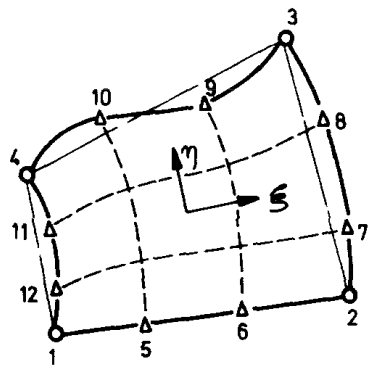
\includegraphics[width=4cm]{images/elements/Q3_12}
\end{center}






%%%%%%%%%%%%%%%%%%%%%%%%%%%%%%%%%%%%%%%%%%%%%%%%%%%%%%%%%%%%%%%%%%%%%%%%%%%%%%%
\subsection{Eight node serendipity basis functions in 2D ($Q_2^{(8)}$)}
\label{sec:serendipity2D}
\index{general}{$Q_2^{(8)}$} 
\index{general}{Serendipity element}

\begin{flushright} {\tiny {\color{gray} basis\_Q28\_2D.tex}} \end{flushright}
%~~~~~~~~~~~~~~~~~~~~~~~~~~~~~~~~~~~~~~~~~~~~~~~~~~~~~~~~~~~~~~~~~~~~~~~~~~~~~~~~~~~~~~~~~~~~~~~~~~

The serendipity elements are those rectangular elements which have no
interior nodes (See for example Reddy \cite[p65]{reddybook2}).
Inside an element a possible local numbering of the nodes is as follows:

\input{tikz/tikz_serendipity2D}

The main difference with the $Q_2$ element resides in the fact that there is 
no node in the middle of the element.
The polynomial representation of the function $\phi$ over the element is then
\[
\phi_h(r,s) = a + br + cs + drs + er^2 + fs^2 + gr^2s + hrs^2
\]
Note that absence of the $r^2s^2$ term which was previously associated 
to the center node. We find that 
\begin{mdframed}[backgroundcolor=blue!5]
\begin{eqnarray}
\bN_0(r,s)&=& \frac{1}{4}(1-r)(1-s)(-r-s-1) \\
\bN_1(r,s)&=& \frac{1}{4}(1+r)(1-s)(r-s-1) \\
\bN_2(r,s)&=& \frac{1}{4}(1+r)(1+s)(r+s-1) \\
\bN_3(r,s)&=& \frac{1}{4}(1-r)(1+s)(-r+s-1) \\
\bN_4(r,s)&=& \frac{1}{2}(1-r^2)(1-s)  \\
\bN_5(r,s)&=& \frac{1}{2}(1+r)  (1-s^2)\\
\bN_6(r,s)&=& \frac{1}{2}(1-r^2)(1+s)  \\
\bN_7(r,s)&=& \frac{1}{2}(1-r)  (1-s^2)
\end{eqnarray}
\end{mdframed}

The basis functions at the mid side nodes are products of a 
second order polynomial parallel to side and 
a linear function perpendicular to the side
while basis functions for corner nodes are modifications of the bilinear
quadrilateral element.

\begin{center}
\includegraphics[width=4cm]{images/basis_Q28_2D/N1}
\includegraphics[width=4cm]{images/basis_Q28_2D/N2}
\includegraphics[width=4cm]{images/basis_Q28_2D/N3}
\includegraphics[width=4cm]{images/basis_Q28_2D/N4}\\
\includegraphics[width=4cm]{images/basis_Q28_2D/N5}
\includegraphics[width=4cm]{images/basis_Q28_2D/N6}
\includegraphics[width=4cm]{images/basis_Q28_2D/N7}
\includegraphics[width=4cm]{images/basis_Q28_2D/N8}\\
{\captionfont Surface representation of the basis functions on the reference element.
{\color{gray} in images/basis\_Q28\_2D/ }}
\end{center}



The first-order derivatives are given by:

\begin{mdframed}[backgroundcolor=blue!5]
\begin{eqnarray}
\frac{\partial \bN_0}{\partial r}(r,s)&=& -\frac{1}{4}(s-1)(2r+s)  \\
\frac{\partial \bN_1}{\partial r}(r,s)&=& -\frac{1}{4}(s-1)(2r-s)  \\
\frac{\partial \bN_2}{\partial r}(r,s)&=& \frac{1}{4}(s+1)(2r+s)  \\
\frac{\partial \bN_3}{\partial r}(r,s)&=& \frac{1}{4}(s+1)(2r-s)  \\
\frac{\partial \bN_4}{\partial r}(r,s)&=& r(s-1)  \\
\frac{\partial \bN_5}{\partial r}(r,s)&=& \frac{1}{2} (1-s^2)  \\
\frac{\partial \bN_6}{\partial r}(r,s)&=& -r(s+1)  \\
\frac{\partial \bN_7}{\partial r}(r,s)&=& -\frac{1}{2} (1-s^2)  
\end{eqnarray}
\end{mdframed}

\begin{mdframed}[backgroundcolor=blue!5]
\begin{eqnarray}
\frac{\partial \bN_0}{\partial s}(r,s)&=& -\frac{1}{4}(r-1)(r+2s) \\
\frac{\partial \bN_1}{\partial s}(r,s)&=& -\frac{1}{4}(r+1)(r-2s) \\
\frac{\partial \bN_2}{\partial s}(r,s)&=&  \frac{1}{4}(r+1)(r+2s) \\
\frac{\partial \bN_3}{\partial s}(r,s)&=&  \frac{1}{4}(r-1)(r-2s) \\
\frac{\partial \bN_4}{\partial s}(r,s)&=& - \frac{1}{2}(1-r^2)\\
\frac{\partial \bN_5}{\partial s}(r,s)&=&  -(r+1)s \\
\frac{\partial \bN_6}{\partial s}(r,s)&=& \frac{1}{2} (1-r^2)\\
\frac{\partial \bN_7}{\partial s}(r,s)&=&  (r-1)s
\end{eqnarray}
\end{mdframed}
These basis functions are used in \stone 52.
An identical approach to arrive at the basis functions is presented in 
\textcite{eriz68} (1968).


%%%%%%%%%%%%%%%%%%%%%%%%%%%%%%%%%%%%%%%%%%%%%%%%%%%%%%%%%%%%%%%%%%%%%%%%%%%%%%%
\subsection{Eight node serendipity basis functions in 2D ($QH8-C1$)}
\label{sec:serendipity2Db}
\index{general}{$QH8-C1$} \index{general}{Serendipity element}

\begin{flushright} {\tiny {\color{gray} \tt basis\_QH8\_2D.tex}} \end{flushright}
%~~~~~~~~~~~~~~~~~~~~~~~~~~~~~~~~~~~~~~~~~~~~~~~~~~~~~~~~~~~~~~~~~~~~~~~~~~~~~~~~~~~~~~~~~~~~~~~~~~

This element is proposed in \textcite{zhxi20} (2020). Two remarks
must be made: 1) Eq.~(29) of their publication which is the definition
of the basis functions contains an error\footnote{
Answer from the author: ``N5 to N8 is missing an A in the denominator and 
the calculation program does not have this problem''}. 
2) The authors use a rather 
uncommon and annoying rotated numbering:
\begin{verbatim}
      y
      |
2=====5=====1             3=====6=====2
|           |             |           |   (r_0,s_0)=(-1,-1)   (r_4,s_4)=( 0,-1)
|           |             |           |   (r_1,s_1)=(+1,-1)   (r_5,s_5)=(+1, 0)
6           8--x          7     +     5   (r_2,s_2)=(+1,+1)   (r_6,s_6)=( 0,+1)
|           |             |           |   (r_3,s_3)=(-1,+1)   (r_7,s_7)=(-1, 0)
|           |             |           |    
3=====7=====4             0=====4=====1
Zhang & Xiang             our numbering
\end{verbatim}

For each element they define (their numbering):
\begin{eqnarray}
A   &=& \frac{1}{2} [ (x_1-x_3)(y_2-y_4)-(x_2-x_4)(y_1-y_3) ] \nn\\
m_x &=& (x_1-x_4)(y_2-y_3)-(x_2-x_3)(y_1-y_4) \nn\\
m_y &=& (x_3-x_4)(y_1-y_2)-(x_1-x_2)(y_3-y_4) \nn
\end{eqnarray}
Note that $A$ is the area of the element, and that in the case when 
the element is a rectangle then $m_x=m_y=0$.
\begin{eqnarray}
\bN_1(r,s)&=& n_1(r,s) +(m_x^2 - m_xm_y + m_y^2)\frac{E(r,s)}{D} \nn\\
\bN_2(r,s)&=& n_2(r,s) +(m_x^2 + m_xm_y + m_y^2)\frac{E(r,s)}{D} \nn\\
\bN_3(r,s)&=& n_3(r,s) +(m_x^2 - m_xm_y + m_y^2)\frac{E(r,s)}{D} \nn\\
\bN_4(r,s)&=& n_4(r,s) +(m_x^2 + m_xm_y + m_y^2)\frac{E(r,s)}{D} \nn\\
\bN_5(r,s)&=& n_5(r,s) -m_x(2Am_x+m_y^2)\frac{E(r,s)}{AD} \nn\\
\bN_6(r,s)&=& n_6(r,s) -m_y(2Am_y+m_x^2)\frac{E(r,s)}{AD} \nn\\
\bN_7(r,s)&=& n_7(r,s) +m_x(-2Am_x+m_y^2)\frac{E(r,s)}{AD} \nn\\
\bN_8(r,s)&=& n_8(r,s) +m_y(-2Am_y+m_x^2)\frac{E(r,s)}{AD} \nn
\end{eqnarray}
with 
\[
E(r,s)=(1-r^2)(1-s^2)
\qquad
D=4(4A^2+m_x^2+m_y^2)
\]
and where the $n_i$ functions are the basis functions of the 'regular' 
8-node element (see Section~\ref{sec:serendipity2D}).

This is implemented in \stone 52.

\todo[inline]{not finished. SHOW CONSISTENCY !! like in paper
email sent to author about mistake.  }

Let us verify consistency:
\begin{eqnarray}
\sum_{i=1}^8 \bN_i(r,s) 
&=& \underbrace{\sum_{i=1}^8 n_i(r,s)}_{=0} + \frac{E(r,s)}{D} 
\left[
(m_x^2 - m_xm_y + m_y^2)
+(m_x^2 + m_xm_y + m_y^2)
+(m_x^2 - m_xm_y + m_y^2)
+(m_x^2 + m_xm_y + m_y^2) \right. \nn\\
&& \left.
-m_x(2Am_x+m_y^2)\frac{1}{A}
-m_y(2Am_y+m_x^2)\frac{1}{A}
+m_x(-2Am_x+m_y^2)\frac{1}{A}
+m_y(-2Am_y+m_x^2)\frac{1}{A}
\right] \nn\\
&=& \frac{E(r,s)}{D}
\left[(4m_x^2 + 4m_y^2) + \frac{1}{A} (-4Am_x^2 - 4A m_y^2) \right]  \\
&=& 0
\end{eqnarray}




%%%%%%%%%%%%%%%%%%%%%%%%%%%%%%%%%%%%%%%%%%%%%%%%%%%%%%%%%%%%%%%%%%%%%%%%%%%%%%%
\subsection{Biquartic basis functions in 2D ($Q_4$) \label{ss:q42d}}
\index{general}{$Q_4$}
\input{basis_Q4}


%%%%%%%%%%%%%%%%%%%%%%%%%%%%%%%%%%%%%%%%%%%%%%%%%%%%%%%%%%%%%%%%%%%%%%%%%%%%%%%
\subsection{Linear basis functions for triangles in 2D ($P_1$)}\label{ss:p1}
\index{general}{$P_1$}

\begin{flushright} {\tiny {\color{gray} basis\_P1\_2D.tex}} \end{flushright}
%~~~~~~~~~~~~~~~~~~~~~~~~~~~~~~~~~~~~~~~~~~~~~~~~~~~~~~~~~~~~~~~~~~~~~~~~~~~~~~~~~~~~~~~~~~~~~~~~~~

Here we do not start from a reference element but consider instead a generic triangle:

\input{tikz/tikz_P1}

This is the simplest 2D element, which is also called linear triangular element.
Velocities (or displacements) $(u^h,v^h)$ in the element are interpolated from nodal velocities
$(u_i,v_i)$ using basis functions $\bN_i$ as follows,
\begin{small}
\[
\vec\upnu^h=
\left(
\begin{array}{c}
u^h(x,y) \\v^h(x,y)
\end{array}
\right)
=
\left(
\begin{array}{c}
\sum\limits_{i=1}^3 \bN_i(x,y) u_i \\
\sum\limits_{i=1}^3 \bN_i(x,y) v_i
\end{array}
\right)
=
\left(
\begin{array}{cccccc}
\bN_1(x,y) & 0 & \bN_2(x,y) & 0 & \bN_3(x,y) & 0\\
0 & \bN_1(x,y) & 0 & \bN_2(x,y) & 0 & \bN_3(x,y)\\
\end{array}
\right)
\cdot
\left(
\begin{array}{c}
u_1 \\ v_1 \\ u_2 \\ v_2 \\ u_3 \\ v_3
\end{array}
\right)
\]
\end{small}
or simply 

For this element, we have three nodes at the vertices of the triangle, which are 
numbered around the element in the counterclockwise direction. 
Each node has two degrees of freedom (i.e. it can move in the $x$ and $y$ directions). 
The velocities $u^h$ and $v^h$ are assumed to be linear functions within the element, that is, 
\begin{eqnarray}
u^h(x,y)&=&b_1 +b_2x+b_3y \nn\\
v^h(x,y)&=&b_4 +b_5x+b_6y
\end{eqnarray}
where $b_i$ are constants to be determined and which depend on the triangle shape.
Note that the strain rate components are then given by
\begin{eqnarray}
\dot\varepsilon_{xx}(\vec\upnu)&=&b_2  \nn\\
\dot\varepsilon_{yy}(\vec\upnu)&=&b_6  \nn\\
\dot\varepsilon_{xy}(\vec\upnu)&=&(b_3+b_5)/2 \nn
\end{eqnarray}
and are constant throughout the element.

The velocities should satisfy the following six equations (when it is evaluated at a node we should 
recover the nodal velocity):
\begin{eqnarray}
u_1 &=& u^h(x_1,y_1)= b_1 + b_2x_1+b_3y_1 \nn\\
u_2 &=& u^h(x_2,y_2)= b_1 + b_2x_2+b_3y_2 \nn\\
u_3 &=& u^h(x_3,y_3)= b_1 + b_2x_3+b_3y_3 \nn\\
v_1 &=& v^h(x_1,y_1)= b_4 + b_5x_1+b_6y_1 \nn\\
v_2 &=& v^h(x_2,y_2)= b_4 + b_5x_2+b_6y_2 \nn\\
v_3 &=& v^h(x_3,y_3)= b_4 + b_5x_3+b_6y_3 \nn
\end{eqnarray}
Let us focus on the three equations with the $u$ component of the velocity.
These can be re-written:
\[
\left(
\begin{array}{c}
u_1 \\ u_2 \\ u_3  
\end{array}
\right)
=
\left(
\begin{array}{ccc}
1 & x_1 & y_1 \\
1 & x_2 & y_2 \\
1 & x_3 & y_3 \\
\end{array}
\right)
\cdot
\left(
\begin{array}{c}
b_1 \\ b_2 \\ b_3  
\end{array}
\right)
\]
In order to obtain $b_1,b_2,b_3$ we need to solve this system, or simply to compute the
inverse of the $3\times 3$ ${\bm M}$ matrix, as explained in Appendix~\ref{sec:inv3x3}.
We define $D={\rm det}({\bm M})$ and we get
\[
\left(
\begin{array}{c}
b_1 \\ b_2 \\ b_3  
\end{array}
\right)
=
\frac{1}{D}
\tilde{\bm M}
\cdot
\left(
\begin{array}{c}
u_1 \\ u_2 \\ u_3  
\end{array}
\right)
%\qquad
%{\rm and}
%\qquad
%\left(
%\begin{array}{c}
%b_4 \\ b_5 \\ b_6  
%\end{array}
%\right)
%=
%\frac{1}{D}
%\tilde{\bm M}
%\cdot
%\left(
%\begin{array}{c}
%v_1 \\ v_2 \\ v_3  
%\end{array}
%\right)
\]
The matrix $\tilde{\bm M}$ is given by:
\[
\tilde{\bm M}
%=
%\left(
%\begin{array}{ccc}
%  x_2y_3-x_3y_2  & -(y_3-y_2) &   x_3-x_2 \\
%-(x_1y_3-x_3y_1) &   y_3-y_1  & -(x_3-x_1) \\
%  x_1y_2-x_2y_1  & -(y_2-y_1) &   x_2-x_1
%\end{array}
%\right)
=
\left(
\begin{array}{ccc}
x_2y_3-x_3y_2 & x_3y_1-x_1y_3 & x_1y_2-x_2y_1 \\
y_2-y_3 & y_3-y_1  & y_1-y_2 \\
x_3-x_2 & x_1-x_3 & x_2-x_1 
\end{array}
\right)
\]
so that 
\begin{eqnarray}
b_1 &=& \frac1D [ (x_2y_3-x_3y_2)u_1 + (x_3y_1-x_1y_3)u_2 + (x_1y_2-x_2y_1)u_3 ] \nn\\
b_2 &=& \frac1D [ (y_2-y_3)u_1 + (y_3-y_1)u_2 + (y_1-y_2)u_3 ] \nn\\
b_3 &=& \frac1D [ (x_3-x_2)u_1 + (x_1-x_3)u_2 + (x_2-x_1)u_3 ]
\end{eqnarray}
We then have
\begin{eqnarray}
u^h(x,y) 
&=& b_1 + b_2 x + b_3 y \nn\\
&=&\frac1D [(x_2y_3-x_3y_2)u_1 + (x_3y_1-x_1y_3)u_2 + (x_1y_2-x_2y_1)u_3 ] \nn\\
&+&\frac1D [(y_2-y_3)u_1 + (y_3-y_1)u_2 + (y_1-y_2)u_3]x \nn\\
&+&\frac1D [(x_3-x_2)u_1 + (x_1-x_3)u_2 + (x_2-x_1)u_3]y \nn\\
&=&\frac1D [(x_2y_3-x_3y_2) + (y_2-y_3)x + (x_3-x_2)y]u_1\nn\\ 
&+&\frac1D [(x_3y_1-x_1y_3) + (y_3-y_1) x + (x_1-x_3) y]u_2 \nn\\
&+&\frac1D [(x_1y_2-x_2y_1) + (y_1-y_2) x + (x_2-x_1) y]u_3\nn\\
&=& \bN_1(x,y) u_1 + \bN_2(x,y) u_2 + \bN_3(x,y) u_3
\end{eqnarray}
with the linear basis functions are given by:
\begin{eqnarray}
\bN_1(x,y) &=& \frac{1}{D}[(x_2y_3-x_3y_2) + (y_2-y_3)x + (x_3-x_2)y] \nn\\
\bN_2(x,y) &=& \frac{1}{D}[(x_3y_1-x_1y_3) + (y_3-y_1)x + (x_1-x_3)y] \nn\\
\bN_3(x,y) &=& \frac{1}{D}[(x_1y_2-x_2y_1) + (y_1-y_2)x + (x_2-x_1)y] \nn
\end{eqnarray}
We can then easily verify that for example
\begin{eqnarray}
\bN_2(x_1,y_1)&=& \frac{1}{D}[(x_3y_1-x_1y_3) + (y_3-y_1)x_1 + (x_1-x_3)y_1] = 0 \\
\bN_2(x_2,y_2)&=& \frac{1}{D}[(x_3y_1-x_1y_3) + (y_3-y_1)x_2 + (x_1-x_3)y_2] = 1 \\
\bN_2(x_3,y_3)&=& \frac{1}{D}[(x_3y_1-x_1y_3) + (y_3-y_1)x_3 + (x_1-x_3)y_3] = 0 
\end{eqnarray}
Note that the area $A$ of the triangle is given by:
\[
A=\frac{1}{2}D = \frac{1}{2}
\left|
\begin{array}{ccc}
1 & x_1 & y_1 \\
1 & x_2 & y_2 \\
1 & x_3 & y_3 
\end{array}
\right|
\]

\noindent If we now consider the reference element in the reduced coordinates space $(r,s)$:

\input{tikz/tikz_P1ref}

The basis polynomial is then
\[
f(r,s) = a + br + cs 
\]
and the basis functions:
\begin{mdframed}[backgroundcolor=blue!5]
\begin{eqnarray}
\bN_0(r,s) &=& 1-r-s \\
\bN_1(r,s) &=& r \\
\bN_2(r,s) &=& s 
\end{eqnarray}
\end{mdframed}
Once again we can verify that $\bN_i(x_j,y_j)=\delta_{ij}$ and $\sum\limits_i \bN_i(r,s)=1$.





%%%%%%%%%%%%%%%%%%%%%%%%%%%%%%%%%%%%%%%%%%%%%%%%%%%%%%%%%%%%%%%%%%%%%%%%%%%%%%%
\subsection{Linear basis functions for quadrilaterals in 2D ($P_1$)}\label{ss:lbfq2D}
\index{general}{$P_1$}

\input{basis_pm1_2D}

%%%%%%%%%%%%%%%%%%%%%%%%%%%%%%%%%%%%%%%%%%%%%%%%%%%%%%%%%%%%%%%%%%%%%%%%%%%%%%%
\subsection{Enriched linear basis functions in triangles ($P_1^+$)}
\index{general}{$P_1^+$}

\input{basis_p1p_2D}

%%%%%%%%%%%%%%%%%%%%%%%%%%%%%%%%%%%%%%%%%%%%%%%%%%%%%%%%%%%%%%%%%%%%%%%%%%%%%%%
\subsection{Quadratic basis functions for triangles in 2D ($P_2$)\label{basis:p2}}
\index{general}{$P_2$}
\begin{flushright} {\tiny {\color{gray} basis\_p2\_2D.tex}} \end{flushright}
%~~~~~~~~~~~~~~~~~~~~~~~~~~~~~~~~~~~~~~~~~~~~~~~~~~~~~~~~~~~~~~~~~~~~~~~~~~~~~~~~~~~~~~~~~~~~~~~~~~

\input{tikz/tikz_P2}

The basis polynomial is then
\[
f(r,s) = c_1 + c_2 r + c_3 s + c_4  r^2 + c_5 rs  + c_6 s^2
\]
We have 
\begin{eqnarray}
f_0 = f(r_0,s_0) &=& c_1 \nonumber\\
f_1 = f(r_1,s_1) &=& c_1 + c_2 + c_4\nonumber\\
f_2 = f(r_2,s_2) &=& c_1 + c_3 + c_6\nonumber\\
f_3 = f(r_3,s_3) &=& c_1 + c_2/2 + c_4/4\nonumber\\
f_4 = f(r_4,s_4) &=& c_1 + c_2/2 + c_3/2  + c_4/4 + c_5/4 + c_6/4\nonumber\\
f_5 = f(r_5,s_5) &=& c_1 + c_3/2 + c_6/4\nonumber
\end{eqnarray}
This can be cast as $\vec{f}={\bm A}\cdot \vec{c}$ where ${\bm A}$ is a $6\times6$ matrix:
\[
{\bm A}=
\left(
\begin{array}{cccccc}
1&0   &  0  & 0   & 0   & 0\\
1&1   &  0  & 1   & 0   & 0\\
1&0   &  1  & 0   & 0   & 1\\
1&1/2 &  0  & 1/4 & 0   & 0\\
1&1/2 &  1/2& 1/4 & 1/4 & 1/4\\
1&0   &  1/2& 0   & 0   & 1/4
\end{array}
\right)
\]
As it turns out it is rather trivial to compute the inverse of this matrix:
\[
{\bm A}^{-1}=
\left(
\begin{array}{cccccc}
1  & 0 & 0  & 0  & 0 & 0  \\
-3 & -1& 0  & 4  & 0 & 0 \\
-3 & 0 & -1 & 0  & 0 & 4 \\
2  & 2 & 0  & -4 & 0 & 0  \\
4  & 0 & 0  & -4 & 4 & -4 \\
2  & 0 & 2  & 0  & 0 & -4
\end{array}
\right)
\]
Using $\vec{c}={\bm A}^{-1}\cdot \vec{f}$ one then obtains:
\begin{eqnarray}
c_1 &=& f_0 \nn\\
c_2 &=& -3f_0-f_1+4f_3\nn\\
c_3 &=& -3f_0-f_2+4f_5  \nn\\
c_4 &=& 2f_0+2f_1-4f_3 \nn\\
c_5 &=& 4f_0-4f_3+4f_4-4f_5 \nn\\
c_6 &=& (2f_0+2f_2-4f_5 \nn
\end{eqnarray}
and then
\begin{eqnarray}
f(r,s) 
&=& f_0 + (-3f_0-f_1+4f_3) r + (-3f_0-f_2+4f_5)s \nonumber\\
&& +(2f_0+2f_1-4f_3)r^2 + (4f_0-4f_3+4f_4-4f_5) rs + (2f_0+2f_2-4f_5)s^2 \nonumber\\
&=& \sum_{i=0}^5 \bN_i(r,s) f_i
\end{eqnarray}
with
\begin{mdframed}[backgroundcolor=blue!5]
\begin{eqnarray}
\bN_0(r,s) &=& 1-3r-3s+2r^2+4rs+2s^2 \nonumber\\
\bN_1(r,s) &=& -r+2r^2 \nonumber\\
\bN_2(r,s) &=& -s+2s^2 \nonumber\\
\bN_3(r,s) &=& 4r-4r^2-4rs \nonumber\\
\bN_4(r,s) &=& 4rs \nonumber\\
\bN_5(r,s) &=& 4s-4rs-4s^2 \nonumber
\end{eqnarray}
\end{mdframed}

The derivatives are as follows:
\begin{eqnarray}
\frac{\partial \bN_0}{\partial r}(r,s) &=&  -3+4r+4s \nn\\ 
\frac{\partial \bN_1}{\partial r}(r,s) &=&  -1+4r\nn\\ 
\frac{\partial \bN_2}{\partial r}(r,s) &=&  0\nn\\ 
\frac{\partial \bN_3}{\partial r}(r,s) &=&  4-8r-4s\nn\\ 
\frac{\partial \bN_4}{\partial r}(r,s) &=&  4s\nn\\ 
\frac{\partial \bN_5}{\partial r}(r,s) &=&  -4s\nn
\end{eqnarray}

\begin{eqnarray}
\frac{\partial \bN_0}{\partial s}(r,s) &=&  -3+4r+4s\nn\\ 
\frac{\partial \bN_1}{\partial s}(r,s) &=&  0\nn\\ 
\frac{\partial \bN_2}{\partial s}(r,s) &=&  -1+4s\nn\\ 
\frac{\partial \bN_3}{\partial s}(r,s) &=&  -4r\nn\\ 
\frac{\partial \bN_4}{\partial s}(r,s) &=&  4r\nn\\ 
\frac{\partial \bN_5}{\partial s}(r,s) &=&  4-4r-8s\nn
\end{eqnarray}


%%%%%%%%%%%%%%%%%%%%%%%%%%%%%%%%%%%%%%%%%%%%%%%%%%%%%%%%%%%%%%%%%%%%%%%%%%%%%%%
\subsection{Enriched quadratic basis functions in triangles ($P_2^+$)}
\index{general}{$P_2^+$}
\begin{flushright} {\tiny {\color{gray} basis\_p2p\_2D.tex}} \end{flushright}
%~~~~~~~~~~~~~~~~~~~~~~~~~~~~~~~~~~~~~~~~~~~~~~~~~~~~~~~~~~~~~~~~~~~~~~~~~~~~~~~~~~~~~~~~~~~~~~~~~~

This is used by the Crouzeix-Raviart element, see Section~\ref{sec:crouzeix-raviart}. 
\index{general}{Crouzeix-Raviart}


\begin{flushright} {\tiny {\color{gray} (tikz\_P2.tex)}} \end{flushright}
%~~~~~~~~~~~~~~~~~~~~~~~~~~~~~~~~~~~~~~~~~~~~~~~~~~~~~~~~~~~~~~~~~~~~~~~~~~~~~~~~~~~~~~~~~~~~~~~~~~

\begin{center}
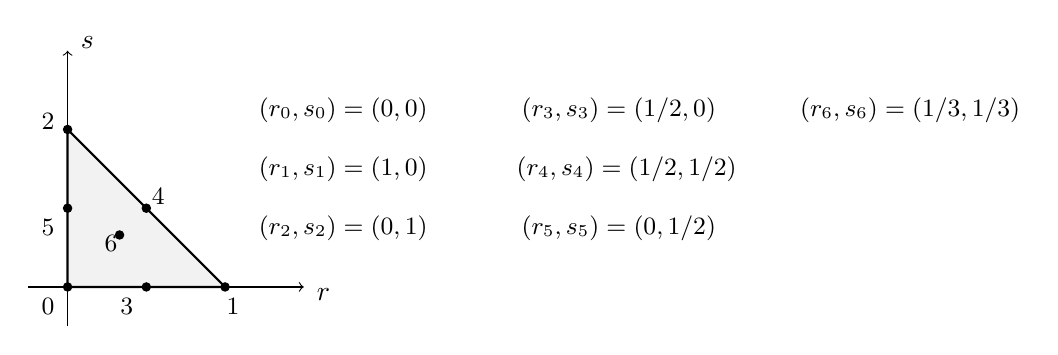
\begin{tikzpicture}
%\draw[step=0.5cm,gray,very thin] (0,0) grid (4,4); 
\draw[fill=gray!10,gray!10] (0.5,0.5)--(2.5,0.5)--(0.5,2.5)--cycle;
\draw[thick] (0.5,0.5)--(2.5,0.5)--(0.5,2.5)--cycle;
\draw [->] (0,0.5) -- (3.5,0.5);
\draw [->] (0.5,0) -- (0.5,3.5);
\node[] at (3.75,0.4) {$r$};
\node[] at (0.75,3.6) {$s$};
\draw[black,fill=black] (0.5,0.5)   circle (1.5pt);
\draw[black,fill=black] (2.5,0.5)   circle (1.5pt);
\draw[black,fill=black] (0.5,2.5)   circle (1.5pt);
\draw[black,fill=black] (1.5,0.5)   circle (1.5pt);
\draw[black,fill=black] (0.5,1.5)   circle (1.5pt);
\draw[black,fill=black] (1.5,1.5)   circle (1.5pt);
\draw[black,fill=black] (1.16,1.16) circle (1.5pt);

\node[] at (0.25,0.25) {\small $0$};
\node[] at (2.6,0.25)  {\small $1$};
\node[] at (0.25,2.6)  {\small $2$};
\node[] at (1.25,0.25) {\small $3$};
\node[] at (1.65,1.65) {\small $4$};
\node[] at (0.25,1.25) {\small $5$};
\node[] at (1.05,1.05)   {\small $6$};

\node[] at (4,2.75) {\small $(r_0,s_0)=(0,0)$};
\node[] at (4,2)    {\small $(r_1,s_1)=(1,0)$};
\node[] at (4,1.25) {\small $(r_2,s_2)=(0,1)$};
\node[] at (7.5,2.75) {\small $(r_3,s_3)=(1/2,0)$};
\node[] at (7.6,2)    {\small $(r_4,s_4)=(1/2,1/2)$};
\node[] at (7.5,1.25) {\small $(r_5,s_5)=(0,1/2)$};
\node[] at (11.2,2.75) {\small $(r_6,s_6)=(1/3,1/3)$};
\end{tikzpicture}
\end{center}



The basis functions are given by:
\todo[inline]{find reference}

\begin{mdframed}[backgroundcolor=blue!5]
\begin{eqnarray}
\bN_0(r,s) &=&  (1-r-s)(1-2r-2s+ 3rs) \\
\bN_1(r,s) &=& r (2 r -1 + 3s-3rs-3s^2 ) \\
\bN_2(r,s) &=& s (2s -1 + 3r-3r^2-3rs )\\
\bN_3(r,s) &=& 4(1-r-s)r(1 -3s ) \\
\bN_4(r,s) &=& 4rs [-2+3r+3s]\\
\bN_5(r,s) &=& 4(1-r-s)s(1-3r)\\
\bN_6(r,s) &=& 27 (1-r-s)rs 
\end{eqnarray}
\end{mdframed}
It is then easy to verify that for all basis functions we have 
$\bN_i(r_j,s_j)=\delta_{ij}$ where $j$ denotes one of the seven nodes. 
The derivatives are as follows:
\begin{eqnarray}
\frac{\partial \bN_0}{\partial r}(r,s) &=& r(4-6s)-3s^2+7s-3\\
\frac{\partial \bN_1}{\partial r}(r,s) &=& r(4-6s)-3s^2+3s-1\\
\frac{\partial \bN_2}{\partial r}(r,s) &=& -3s(2r+s-1)  \\
\frac{\partial \bN_3}{\partial r}(r,s) &=& 4(3s-1)(2r+s-1) \\
\frac{\partial \bN_4}{\partial r}(r,s) &=& 4s(6r+3s-2) \\
\frac{\partial \bN_5}{\partial r}(r,s) &=& 4s(6r+3s-4)\\
\frac{\partial \bN_6}{\partial r}(r,s) &=& -27s(2r+s-1)
\end{eqnarray}

\begin{eqnarray}
\frac{\partial \bN_0}{\partial s}(r,s) &=& -3r^2+r(7-6s)+4s-3\\
\frac{\partial \bN_1}{\partial s}(r,s) &=& -3r(r+2s-1)\\
\frac{\partial \bN_2}{\partial s}(r,s) &=& -3r^2+r(3-6s)+4s-1 \\
\frac{\partial \bN_3}{\partial s}(r,s) &=& 4r(3r+6s-4)  \\
\frac{\partial \bN_4}{\partial s}(r,s) &=& 4r(3r+6s-2) \\
\frac{\partial \bN_5}{\partial s}(r,s) &=& 4(3r-1)(r+2s-1)\\
\frac{\partial \bN_6}{\partial s}(r,s) &=& -27r(r+2s-1)
\end{eqnarray}

Note that the basis functions can also be expressed as a function of the barycentric coordinates, 
as in the MILAMIN code \cite{daks08} or in Cuvelier \etal (1986) \cite{cuss86}\footnote{Note
that the numbering of the nodes in the book is different with respect to the one above. }

\begin{eqnarray}
N_0(\lambda_1,\lambda_2,\lambda_3) &=& \eta_1(2\eta_1-1)+ 3\eta_1\eta_2\eta_3\\
N_1(\lambda_1,\lambda_2,\lambda_3) &=& \eta_2(2\eta_2-1)+ 3\eta_1\eta_2\eta_3\\
N_2(\lambda_1,\lambda_2,\lambda_3) &=& \eta_3(2\eta_3-1)+ 3\eta_1\eta_2\eta_3\\
N_3(\lambda_1,\lambda_2,\lambda_3) &=& 4\eta_2\eta_3 - 12\eta_1\eta_2\eta_3\\
N_4(\lambda_1,\lambda_2,\lambda_3) &=& 4\eta_1\eta_3 - 12\eta_1\eta_2\eta_3\\
N_5(\lambda_1,\lambda_2,\lambda_3) &=& 4\eta_1\eta_2 - 12\eta_1\eta_2\eta_3\\
N_6(\lambda_1,\lambda_2,\lambda_3) &=& 27\eta_1\eta_2\eta_3 
\end{eqnarray}

\todo[inline]{
VERIFY that when $\eta_1=1-r-s$, $\eta_2=r$ and $\eta_3=s$ we find the above $r,s$ basis functions
}


%1-4*eta1+3*eta1*eta3-3*eta2*eta3 ...
%-1+4*eta2+3*eta1*eta3-3*eta2*eta3 ...
%3*eta1*eta3-3*eta2*eta3 ...
%4*eta3+12*eta2*eta3-12*eta1*eta3 ...
%-4*eta3+12*eta2*eta3-12*eta1*eta3 ...
%4*eta1-4*eta2+12*eta2*eta3-12*eta1*eta3 ...
%-27*eta2*eta3+27*eta1*eta3

%1-4*eta1+3*eta1*eta2-3*eta2*eta3 ...
%+3*eta1*eta2-3*eta2*eta3 ...
%-1+4*eta3+3*eta1*eta2-3*eta2*eta3 ...
%4*eta2-12*eta1*eta2+12*eta2*eta3 ...
%4*eta1-4*eta3-12*eta1*eta2+12*eta2*eta3 ...
%-4*eta2-12*eta1*eta2+12*eta2*eta3 ...
%27*eta1*eta2-27*eta2*eta3];  




%%%%%%%%%%%%%%%%%%%%%%%%%%%%%%%%%%%%%%%%%%%%%%%%%%%%%%%%%%%%%%%%%%%%%%%%%%%%%%%
\subsection{Cubic basis functions for triangles ($P_3$) \label{basis:p3}}
\index{general}{$P_3$}
\begin{flushright} {\tiny {\color{gray} basis\_p3\_2D.tex}} \end{flushright}
%~~~~~~~~~~~~~~~~~~~~~~~~~~~~~~~~~~~~~~~~~~~~~~~~~~~~~~~~~~~~~~~~~~~~~~~~~~~~~~~~~~~~~~~~~~~~~~~~~~

\todo[inline]{TIKZ!}
\begin{verbatim}
9
|\          (r_0,s_0)=(0,0)    (r_5,s_5)=(1/3,1/3)
|  \        (r_1,s_1)=(1/3,0)  (r_6,s_6)=(2/3,1/3)
7   8       (r_2,s_2)=(2/3,0)  (r_7,s_7)=(0,2/3)
|    \      (r_3,s_3)=(1,0)    (r_8,s_8)=(1/3,2/3)
4  5   6    (r_4,s_4)=(0,1/3)  (r_9,s_9)=(0,1)
|       \ 
0==1==2==3
\end{verbatim}
The basis polynomial is then
\[
f(r,s) = c_0 + c_1 r+ c_2 s + c_3r^2 + c_4 rs + c_5 s^2
+c_6 r^3 + c_7 r^2s + c_8 rs^2 + c_9 s^3
\]
with the support nodes being given by 

\begin{eqnarray}
(r_0,s_0) &=& (0,0) \\
(r_1,s_1) &=& (1/3,0) \\
(r_2,s_2) &=& (2/3,0) \\
(r_3,s_3) &=& (1,0) \\
(r_4,s_4) &=& (0,1/3) \\
(r_5,s_5) &=& (1/3,1/3) \\
(r_6,s_6) &=& (2/3,1/3) \\
(r_7,s_7) &=& (0,2/3) \\
(r_8,s_8) &=& (1/3,2/3) \\
(r_9,s_9) &=& (0,1) 
\end{eqnarray}


\begin{eqnarray}
f_0 = f(r_0,s_0) &=& c_0 \nn\\
f_1 = f(r_1,s_1) &=& c_0 + c_1 + \frac19 c_3 + \frac{1}{27} c_6 \nn\\
f_2 = f(r_2,s_2) &=& c_0 + \frac23 c_1 + \frac{4}{9} c_3 + \frac{8}{27} c_6\nn\\
f_3 = f(r_3,s_3) &=& c_0 + c_1 + c_3 + c_6 \nn\\
f_4 = f(r_4,s_4) &=& c_0 + \frac13 c_2   + \frac19 c_5 + \frac{1}{27} c_9 \nn\\
f_5 = f(r_5,s_5) &=& c_0 + \frac13 c_1 + \frac13 c_2 + \frac19 c_3 
+ \frac19 c_4  + \frac19 c_5 + \frac{1}{27}c_6 r^3 + \frac{1}{27}c_7 + \frac{1}{27}c_8 + \frac{1}{27} c_9 \nn\\
f_6 = f(r_6,s_6) &=& c_0 + \frac23 c_1 + \frac13 c_2  
+ \frac49 c_3+ \frac29 c_4 + \frac19 c_5 + \frac{8}{27}c_6 +\frac{4}{27} c_7 +\frac{2}{27} c_8 +\frac19 c_9 \nn\\
f_7 = f(r_7,s_7) &=& c_0 + \frac23 c_2  + \frac49c_5 + \frac{8}{27}c_9 \nn\\
f_8 = f(r_8,s_8) &=& c_0 + \frac13c_1 + \frac23 c_2 + \frac19 c_3
+ \frac29 c_4  + \frac49 c_5 
+ \frac{1}{27}c_6  + \frac{2}{27}c_7  + \frac{4}{27}c_8 + \frac{8}{27}c_9 s^3 \nn\\
f_9 = f(r_9,s_9) &=& c_0 + c_2 + c_5 + c_9 \nn 
\end{eqnarray}
or,
\[
\left(
\begin{array}{cccccccccc}
1 & 0& 0&0&0&0&0&0&0&0 \\
1 & \frac13 & 0 & \frac19 &0 &0 & \frac{1}{27} & 0 & 0 & 0 \\
1 & \frac23 & 0 & \frac49 & 0 & 0 & \frac{8}{27} &0 &0 &0   \\
1 & 1 & 0 & 1 &0 & 0 &1 &0 &0 &0    \\
1 & 0 & \frac13 & 0 & 0 & \frac19 & 0& 0& 0 & \frac{1}{27}\\
1 & \frac13 & \frac13 & \frac19 & \frac19 & \frac19 & \frac{1}{27} & \frac{1}{27} & \frac{1}{27} & \frac{1}{27}    \\
1 & \frac23 & \frac13 & \frac49 & \frac29 & \frac19 
& \frac{8}{27}  & \frac{4}{27}  & \frac{2}{27}  & \frac{1}{27}    \\
1 & 0 & \frac23 & 0 & 0 & \frac49 & 0& 0& 0& \frac{8}{27}  \\
1 & \frac13 & \frac23 & \frac19 & \frac29 & \frac49 & \frac{1}{27} & \frac{2}{27} & \frac{4}{27} & \frac{8}{27}    \\
1 & 0 & 1 & 0 & 0 &1 & 0 & 0 & 0 & 1   
\end{array}
\right)
\cdot
\left(
\begin{array}{c}
c_0 \\ c_1 \\ c_2 \\ c_3 \\ c_4 \\ c_5 \\ c_6 \\ c_7 \\ c_8 \\ c_9
\end{array}
\right)
=
\left(
\begin{array}{c}
f_0 \\ f_1 \\ f_2 \\ f_3 \\ f_4 \\ f_5 \\ f_6 \\ f_7 \\ f_8 \\ f_9
\end{array}
\right)
\]
or, 
\[
\frac{1}{27}
\left(
\begin{array}{cccccccccc}
27 & 0& 0&0&0&0&0&0&0&0 \\
27 & 9 & 0 & 3 &0 &0 & 1 & 0 & 0 & 0 \\
27 & 18 & 0 & 12 & 0 & 0 & 8 &0 &0 &0   \\
27 & 27 & 0 & 27 &0 & 0 &27 &0 &0 &0    \\
27 & 0 & 9 & 0 & 0 & 3 & 0& 0& 0 & 1\\
27 & 9 & 9 & 3 & 3 & 3 & 1 & 1 & 1 & 1    \\
27 & 18 & 9 & 12 & 6 & 3 & 8  & 4  & 2  & 1    \\
27 & 0 & 18 & 0 & 0 & 12 & 0& 0& 0& 8  \\
27 & 9 & 18 & 3 & 6 & 12 & 1 & 2 & 4 & 8\\
27 & 0 & 27 & 0 & 0 &27 & 0 & 0 & 0 & 27  
\end{array}
\right)
\cdot
\left(
\begin{array}{c}
c_0 \\ c_1 \\ c_2 \\ c_3 \\ c_4 \\ c_5 \\ c_6 \\ c_7 \\ c_8 \\ c_9
\end{array}
\right)
=
\left(
\begin{array}{c}
f_0 \\ f_1 \\ f_2 \\ f_3 \\ f_4 \\ f_5 \\ f_6 \\ f_7 \\ f_8 \\ f_9
\end{array}
\right)
\]
The inverse of the matrix is 
\[
\frac12
\left(
\begin{array}{cccccccccc}
2 &0 &0 &0 &0 &0 &0 &0 &0 &0\\
-11 & 18 & -9 & 2 &0 &0 &0 &0 &0 & 0 \\
-11 & 0 & 0 & 0 & 18 & 0 & 0 & -9 & 0 & 2 \\
18 & -45 & 36 &-9 &  0& 0& 0& 0& 0& 0 \\
36 &-45 & 9 & 0 &  -45 & 54 &-9 & 9 &  -9 & 0\\
18 &0& 0& 0 & -45& 0 &0 & 36& 0 &-9 \\
-9 & 27 &-27 & 9 &  0 & 0 & 0 & 0  &  0 & 0\\
-27 & 54& -27& 0& 27 &-54 & 27 &0 &0 &0 \\
-27 & 27 &0 &0 &54& -54 &0 &-27  &  27 &0 \\
-9 &0 &0 &0 &27 &0& 0 &-27 &0&  9
\end{array}
\right)
\]
so that the solution of the system ${\bm A}\cdot \vec{c}=\vec{f}$ is
$\vec{c} = {\bm A}^{-1}\cdot \vec{f}$, or:
\begin{eqnarray}
c_0 &=& 1   \nn\\
c_1 &=& \frac12 (-11 f_0 + 18 f_1 -9 f_2 + 2f_3 ) \nn\\
c_2 &=& \frac12 (-11f_0 + 18f_4 -9 f_7 + 2f_9) \nn\\
c_3 &=& \text{etc ...}
\end{eqnarray}
which we insert in 
\[
f(r,s) = c_0 + c_1 r+ c_2 s + c_3r^2 + c_4 rs + c_5 s^2
+c_6 r^3 + c_7 r^2s + c_8 rs^2 + c_9 s^3
\]
and we then obtain
\begin{eqnarray}
f(r,s) 
&=&\frac12\left(2-11r-11s+18r^2+36rs+18s^2-9r^3-27r^2s-27rs^2-9s^3 \right) f_0 \nn\\
&+&\frac12\left(18r-45r^2-45rs +27r^3 +54r^2s+27rs^2\right) f_1\nn\\
&+&\frac12\left( -9r+36r^2+9rs -27r^3 -27r^2s \right) f_2\nn\\
&+&\frac12\left( 2r-9r^2+9r^3 \right) f_3\nn\\
&+&\frac12\left( 18s -45rs-45s^2+27r^2s+54rs^2+27s^3\right) f_4\nn\\
&+&\frac12\left( 54rs-54r^2s-54rs^2  \right) f_5\nn\\
&+&\frac12\left( -9rs+27r^2s  \right) f_6\nn\\
&+&\frac12\left( -9s+9rs+36s^2-27rs^2-27s^3  \right) f_7\nn\\
&+&\frac12\left( -9rs+27rs^2  \right) f_8\nn\\
&+&\frac12\left( 2s-9s^2+9s^3  \right) f_9 \nn \\
&=& \sum_{i=0}^9 \bN_i(r,s) f_i \nn
\end{eqnarray}


\begin{eqnarray}
\bN_0(r,s) &=& \frac12\left(2-11r-11s+18r^2+36rs+18s^2-9r^3-27r^2s-27rs^2-9s^3 \right)   \nn\\
\bN_1(r,s)&=& \frac12\left(18r-45r^2-45rs +27r^3 +54r^2s+27rs^2\right)   \nn\\
\bN_2(r,s)&=& \frac12\left( -9r+36r^2+9rs -27r^3 -27r^2s \right)   \nn\\
\bN_3(r,s)&=& \frac12\left( 2r-9r^2+9r^3 \right)   \nn\\
\bN_4(r,s)&=& \frac12\left( 18s -45rs-45s^2+27r^2s+54rs^2+27s^3\right) \nn\\
\bN_5(r,s)&=& \frac12\left( 54rs-54r^2s-54rs^2  \right)   \nn\\
\bN_6(r,s)&=& \frac12\left( -9rs+27r^2s  \right)   \nn\\
\bN_7(r,s)&=& \frac12\left( -9s+9rs+36s^2-27rs^2-27s^3\right)\nn\\
\bN_8(r,s)&=& \frac12\left( -9rs+27rs^2  \right)   \nn\\
\bN_9(r,s)&=& \frac12\left( 2s-9s^2+9s^3  \right)   
\end{eqnarray}
and then
\begin{eqnarray}
\frac{\partial\bN_0}{\partial r} (r,s) &=& \frac12(-11+36r+36s-27r^2-54rs-27s^2)   \nn\\
\frac{\partial\bN_1}{\partial r} (r,s) &=& \frac12(18-90r-45s+81r^2+108rs+27s^2)   \nn\\
\frac{\partial\bN_2}{\partial r} (r,s) &=& \frac12(-9+72r+9s-81r^2-54rs)   \nn\\
\frac{\partial\bN_3}{\partial r} (r,s) &=& \frac12(2-18r+27r^2)   \nn\\
\frac{\partial\bN_4}{\partial r} (r,s) &=& \frac12(-45s+54rs+54s^2)   \nn\\
\frac{\partial\bN_5}{\partial r} (r,s) &=& \frac12(54s-108rs-54s^2) \nn\\
\frac{\partial\bN_6}{\partial r} (r,s) &=& \frac12(-9s+54rs) \nn\\
\frac{\partial\bN_7}{\partial r} (r,s) &=& \frac12(9s-27s^2) \nn\\
\frac{\partial\bN_8}{\partial r} (r,s) &=& \frac12(-9s+27s^2)\nn\\
\frac{\partial\bN_9}{\partial r} (r,s) &=&  0  \nn
\end{eqnarray}

\begin{eqnarray}
\frac{\partial\bN_0}{\partial s} (r,s) &=& \frac12(-11+36r+36s-27r^2-54rs-27s^2)   \nn\\
\frac{\partial\bN_1}{\partial s} (r,s) &=& \frac12(-45r+54r^2+54rs)   \nn\\
\frac{\partial\bN_2}{\partial s} (r,s) &=& \frac12(9r-27r^2)   \nn\\
\frac{\partial\bN_3}{\partial s} (r,s) &=& 0   \nn\\
\frac{\partial\bN_4}{\partial s} (r,s) &=& \frac12(18-45r-90s+27r^2+108rs+81s^2)   \nn\\
\frac{\partial\bN_5}{\partial s} (r,s) &=& \frac12(54r-54r^2-108rs)   \nn\\
\frac{\partial\bN_6}{\partial s} (r,s) &=& \frac12(-9r+27r^2)   \nn\\
\frac{\partial\bN_7}{\partial s} (r,s) &=& \frac12(-9+9r+72s-54rs-81s^2)   \nn\\
\frac{\partial\bN_8}{\partial s} (r,s) &=& \frac12(-9r+54rs)   \nn\\
\frac{\partial\bN_9}{\partial s} (r,s) &=& \frac12(2-18s+27s^2)   \nn
\end{eqnarray}

It is implemented in \stone~120.
See also python code in {\tt images/basis\_P3} which I wrote to test these basis functions.




















%%%%%%%%%%%%%%%%%%%%%%%%%%%%%%%%%%%%%%%%%%%%%%%%%%%%%%%%%%%%%%%%%%%%%%%%%%%%%%%
\subsection{Quartic basis functions for triangles ($P_4$)}
\index{general}{$P_4$}
\begin{flushright} {\tiny {\color{gray} basis\_p4\_2D.tex}} \end{flushright}
%~~~~~~~~~~~~~~~~~~~~~~~~~~~~~~~~~~~~~~~~~~~~~~~~~~~~~~~~~~~~~~~~~~~~~~~~~~~~~~~~~~~~~~~~~~~~~~~~~~

It is implemented in \stone~120.
See also python code in {\tt images/basis\_P4} which I wrote to test these basis functions.

\begin{flushright} {\tiny {\color{gray} (tikz\_p4.tex)}} \end{flushright}
%~~~~~~~~~~~~~~~~~~~~~~~~~~~~~~~~~~~~~~~~~~~~~~~~~~~~~~~~~~~~~~~~~~~~~~~~~~~~~~~~~~~~~~~~~~~~~~~~~~

\begin{center}
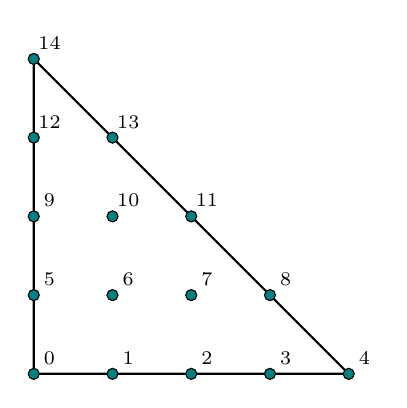
\begin{tikzpicture}
%\draw[step=0.5cm,gray,very thin] (0,0) grid (5,3.5); %bckgr grid
\draw[thick] (0,0) -- (4,0)  -- (0,4) -- cycle; 

\draw[black,fill=teal] (0,0) circle (2pt);
\draw[black,fill=teal] (1,0) circle (2pt);
\draw[black,fill=teal] (2,0) circle (2pt);
\draw[black,fill=teal] (3,0) circle (2pt);
\draw[black,fill=teal] (4,0) circle (2pt);
\draw[black,fill=teal] (0,1) circle (2pt);
\draw[black,fill=teal] (1,1) circle (2pt);
\draw[black,fill=teal] (2,1) circle (2pt);
\draw[black,fill=teal] (3,1) circle (2pt);
\draw[black,fill=teal] (0,2) circle (2pt);
\draw[black,fill=teal] (1,2) circle (2pt);
\draw[black,fill=teal] (2,2) circle (2pt);
\draw[black,fill=teal] (0,3) circle (2pt);
\draw[black,fill=teal] (1,3) circle (2pt);
\draw[black,fill=teal] (0,4) circle (2pt);

\node[] at (0.2,0.2) {\scriptsize $0$};
\node[] at (1.2,0.2) {\scriptsize $1$};
\node[] at (2.2,0.2) {\scriptsize $2$};
\node[] at (3.2,0.2) {\scriptsize $3$};
\node[] at (4.2,0.2) {\scriptsize $4$};
\node[] at (0.2,1.2) {\scriptsize $5$};
\node[] at (1.2,1.2) {\scriptsize $6$};
\node[] at (2.2,1.2) {\scriptsize $7$};
\node[] at (3.2,1.2) {\scriptsize $8$};
\node[] at (0.2,2.2) {\scriptsize $9$};
\node[] at (1.2,2.2) {\scriptsize $10$};
\node[] at (2.2,2.2) {\scriptsize $11$};
\node[] at (0.2,3.2) {\scriptsize $12$};
\node[] at (1.2,3.2) {\scriptsize $13$};
\node[] at (0.2,4.2) {\scriptsize $14$};

\end{tikzpicture}
\end{center}


The support nodes coordinates are as follows:

\begin{center}
\begin{tabular}{cccccccccccccccc}
\hline
$i\rightarrow$& 0& 1 &2 &3 &4 &5 &6 &7 &8 &9 &10 &11 &12 &13 &14  \\
\hline\hline
$r_i$&0&$\frac14$ & $\frac12$ & $\frac34$ & 1 &0 &$\frac14$&$\frac12$&
$\frac34$&0&$\frac14$&$\frac12$&0&$\frac14$&0    \\
$s_i$&0&0&0&0&0&$\frac14$&$\frac14$&$\frac14$&$\frac14$
&$\frac12$&$\frac12$&$\frac12$
&$\frac34$&$\frac34$&1\\
\hline
\end{tabular}
\end{center}

Inside the element a field $f$ is represented by a 4-th order polynomial:
\begin{eqnarray}
f^h(r,s)
&=&c_0 + c_1 r+c_2 s \nn\\
&&+ c_3 r^2 + c_4 rs + c_5 s^2 \nn\\
&&+c_6r^3 + c_7 r^2s + c_8 rs^2 + c_9 s^3 \nn\\
&&
+ c_{10} r^4 
+ c_{11} r^3s 
+ c_{12} r^2s^2
+ c_{13} rs^3
+c_{14} s^4
\end{eqnarray}

At each node the function takes a value $f_i$, $i\in[0,14]$ so that we have:
\[
\left(
\begin{array}{lllllllllllllll}
1\quad{} &0 & 0\quad{}& 0  &0&0\quad{} &0 &0&0&0\quad{} &0& 0&0&0&0\\
1 & \frac14&0&\frac{1}{16}&0&0&\frac{1}{64}&0&0&0&\frac{1}{256}&0&0&0&0 \\
1 & \frac12&0&\frac14&0&0&\frac18&0&0&0&\frac{1}{16}&0&0&0&0 \\
1 & \frac34&0&\frac{9}{16}&0&0&\frac{27}{64}&0&0&0&\frac{81}{256}&0&0&0&0 \\ 
1 &1&0&1&0&0&1&0&0&0&1&0&0&0&0 \\ \\
1 &0&\frac14&0&0&\frac{1}{16}&0&0&0&\frac{1}{64}&0&0&0&0&\frac{1}{256} \\
1 &\frac14&\frac14&\frac{1}{16}&\frac{1}{16}&\frac{1}{16}&\frac{1}{64}&\frac{1}{64}&\frac{1}{64}&\frac{1}{64}&\frac{1}{256}&\frac{1}{256}&\frac{1}{256}&\frac{1}{256}&\frac{1}{256} \\
1 &\frac12&\frac14&\frac14&\frac18&\frac{1}{16}&\frac18&\frac{1}{16}&\frac{1}{32}&\frac{1}{64}&\frac{1}{16}&\frac{1}{32}&\frac{1}{64}&\frac{1}{128}&\frac{1}{256} \\
1 &\frac34&\frac14&\frac{9}{16}&\frac{3}{16}&\frac{1}{16}&\frac{27}{64}&\frac{9}{64}&\frac{3}{64}&\frac{1}{64}&\frac{81}{256}&\frac{27}{256}&\frac{9}{256}&\frac{3}{256}&\frac{1}{256} \\
\\
1 &0&\frac12&0&0&\frac14&0&0&0&\frac18&0&0&0&0&\frac{1}{16} \\
1 &\frac14&\frac12&\frac{1}{16}&\frac{1}{8}&\frac{1}{4}&\frac{1}{64}&\frac{1}{32}&\frac{1}{16}&\frac{1}{8}&\frac{1}{256}&\frac{1}{128}&\frac{1}{64}&\frac{1}{32}&\frac{1}{16} \\
1 &\frac12&\frac12&\frac14&\frac14&\frac14&\frac{1}{8}&\frac{1}{8}&\frac{1}{8}&\frac{1}{8}&\frac{1}{16}&\frac{1}{16}&\frac{1}{16}&\frac{1}{16}&\frac{1}{16} \\ \\
1 &0&\frac34&0&0&\frac{9}{16}&0&0&0&\frac{27}{64}&0&0&0&0&\frac{81}{256} \\
1 &\frac14&\frac34&\frac{1}{16}&\frac{3}{16}&\frac{9}{16}&\frac{1}{64}&\frac{3}{64}&\frac{9}{64}&\frac{27}{64}&\frac{1}{256}&\frac{3}{256}&\frac{9}{256}&\frac{27}{256}&\frac{81}{256} \\ \\
1 &0&1&0&0&1&0&0&0&1&0&0&0&0&1 
\end{array}
\right)
\cdot
\left(
\begin{array}{c}
c_0 \\ \\
c_1 \\
c_2 \\ \\
c_3 \\
c_4 \\
c_5 \\  \\
c_6 \\
c_7 \\
c_8 \\
c_9 \\ \\
c_{10} \\ 
c_{11} \\
c_{12} \\
c_{13} \\
c_{14} 
\end{array}
\right)
=
\left(
\begin{array}{c}
f_0 \\ \\
f_1 \\
f_2 \\ \\
f_3 \\
f_4 \\
f_5 \\ \\
f_6 \\
f_7 \\
f_8 \\
f_9 \\ \\
f_{10} \\
f_{11} \\
f_{12} \\
f_{13} \\
f_{14} 
\end{array}
\right)
\]
or, 

\[
\frac{1}{256}
\left(
\begin{array}{lllllllllllllll}
256\qquad{} &0 & 0\qquad{}& 0  &0&0\qquad{} &0 &0&0&0\quad{} &0& 0&0&0&0\\
256 &64 &0&16 &0&0&4  &0&0&0&1&0&0&0&0 \\
256 &128&0&64 &0&0&32 &0&0&0&16&0&0&0&0 \\
256 &192&0&144&0&0&108&0&0&0&81&0&0&0&0 \\
256 &256&0&256&0&0&256&0&0&0&256&0&0&0&0 \\ 
\\
256 &0  &64&0&0&16& 0&0&0&4 &0&0&0&0&1\\
256 &64 &64&16&16&16& 4&4&4&4 &1&1&1&1&1\\
256 &128&64&64&32&16& 32&16&8&4 &16&8&4&2&1\\
256 &192&64&144&48&16& 108&36&12&4 &81&27&9&3&1\\
\\
256 & 0  &128&0 &0 &64& 0 & 0 & 0 & 32&0&0&0&0&16\\
256 & 64 &128&16&32&64& 4& 8 &16 &32  &1&2&4&8&16\\
256 & 128&128&64&64&64& 32&32&32&32 & 16&16&16&16&16\\
\\
256 & 0 & 192 & 0 & 0 & 144 & 0 & 0 & 0 & 108 & 0 & 0 & 0 & 0 & 81 \\ 
256 & 64 & 192 & 16 & 48 & 144 & 4 & 12 & 36 & 108 & 1 & 3 & 9 & 27 & 81
\\ \\
256 & 0 & 256 & 0 & 0 & 256 & 0 & 0 & 0 & 256 & 0&0 & 0 & 0 & 256
\end{array}
\right)
\cdot
\left(
\begin{array}{c}
c_0 \\ \\
c_1 \\
c_2 \\ \\
c_3 \\
c_4 \\
c_5 \\  \\
c_6 \\
c_7 \\
c_8 \\
c_9 \\ \\
c_{10} \\ 
c_{11} \\
c_{12} \\
c_{13} \\
c_{14} 
\end{array}
\right)
=
\left(
\begin{array}{c}
f_0 \\ \\
f_1 \\
f_2 \\ \\
f_3 \\
f_4 \\
f_5 \\ \\
f_6 \\
f_7 \\
f_8 \\
f_9 \\ \\
f_{10} \\
f_{11} \\
f_{12} \\
f_{13} \\
f_{14} 
\end{array}
\right)
\]


The inverse of the matrix is:
\begin{scriptsize}
\[
\frac13 
\left(
\begin{array}{lllllllllllllll}
3 & 0& 0 &  0 &  0 &  0 &  0 & 0 & 0 &0 &  0 &  0 & 0 &  0  &  0 \\ \\
-25&   48&  -36&   16&   -3&   0&    0&    0&    0&   0& 0&  0& 0& 0& 0\\
-25& 0& 0& 0& 0&   48&    0&    0&    0&  -36& 0& 0& 16& 0&   -3\\ \\
70& -208&  228& -112&   22&    0&0&0&0&0&0&0&0& 0& 0\\
140& -208&   84&  -16& 0& -208& 288&  -96& 16& 84& -96& 12& -16&16&   0\\
70&   0&   0&   0&   0& -208&   0&   0&   0&  228&   0&0& -112& 0&  22\\ \\
-80&  288& -384&  224&  -48&    0&    0&    0&  0&  0& 0& 0& 0& 0&  0\\
-240&  576& -432& 96& 0& 288& -672& 480& -96& -48& 96&  -48& 0& 0& 0\\
-240&  288& -48& 0& 0&  576& -672& 96& 0& -432& 480& -48& 96&  -96& 0\\ 
-80& 0&  0&  0 &   0&  288&    0&    0&    0& -384& 0&  0& 224& 0& -48\\ \\
32& -128&  192& -128&   32&   0&  0&   0&   0& 0&   0&  0& 0&  0& 0\\
128& -384 & 384 &-128&   0& -128&  384& -384&  128& 0& 0&  0& 0& 0&  0\\
192& -384&  192&  0&   0& -384&  768& -384&  0&  192& -384&  192& 0& 0& 0\\
128& -128  &0&  0&    0& -384&  384&   0&   0&  384& -384&   0&
  -128&  128&   0\\
32& 0&  0&   0& 0& -128&  0& 0& 0&  192& 0&  0& -128& 0&   32
\end{array}
\right)
\]
\end{scriptsize}
so that we obtain
\begin{scriptsize}
\begin{eqnarray}
f(r,s) 
&=&\frac13 ( 3-25r-25s+70r^2+140rs+70s^2 -80r^3-240r^2s-240rs^2-80s^3+32r^4 + 128 r^3s + 192 r^2s^2 + 128 rs^3 + 32 s^4 )f_0 \nn\\
&+&\frac13 ( 48r -208r^2-208rs +288r^3+576r^2s+288rs^2-128r^4-384r^3s-384r^2s^2-128rs^3)f_1 \nn\\
&+&\frac13 ( -36r +228r^2+84rs -384r^3-432r^2s-48rs^2+192r^4+384r^3s+192r^2s^2)f_2 \nn\\
&+&\frac13 ( 16r -112r^2-16rs +224r^3+96r^2s-128r^4-128r^3s)f_3 \nn\\
&+&\frac13 ( -3r +22r^2 -48r^3+32r^4)f_4 \nn\\
&+&\frac13 ( 48s -208rs-208s^2 +288r^2s+576rs^2+288s^3-128r^3s-384r^2s^2-384rs^3-128s^4)f_5 \nn\\
&+&\frac13 ( 288rs -672r^2s-672rs^2+384r^3s+768r^2s^2+384rs^3 )f_6 \nn\\
&+&\frac13 ( -96rs +480r^2s+96rs^2-384r^3s-384r^2s^2)f_7 \nn\\
&+&\frac13 ( 16rs -96r^2s+128r^3s   )f_8 \nn\\
&+&\frac13 ( -36s+84rs+228s^2 -48r^2s-432rs^2-384s^3 +192r^2s^2+384rs^3+192s^4)f_9 \nn\\
&+&\frac13 ( -96rs+96r^2s+480rs^2-384r^2s^2-384rs^3 )f_{10} \nn\\
&+&\frac13 ( 12rs-48r^2s-48rs^2+192r^2s^2 )f_{11} \nn\\
&+&\frac13 ( 16s-16rs-112s^2+96rs^2+224s^3-128rs^3-128s^4 )f_{12} \nn\\
&+&\frac13 ( 16rs-96rs^2+128rs^3 )f_{13} \nn\\
&+&\frac13 (-3s+22s^2-48s^3+32s^4  )f_{14} \nn\\
&=& \sum_{i=0}^{14} \bN_i(r,s) f_i
\end{eqnarray}
\end{scriptsize}




and then
\begin{eqnarray}
\frac{\partial\bN_0}{\partial r} (r,s) &=& 
\frac13 ( -25+140r+140s -240r^2-480rs-240s^2+128r^3+384 r^2s + 384 rs^2 + 128 s^3 ) \nn\\
\frac{\partial\bN_1}{\partial r} (r,s) &=& \frac13 ( 48 -416r-208s +864r^2+1152rs+288s^2-512r^3-1152r^2s-768rs^2-128s^3)\nn\\
\frac{\partial\bN_2}{\partial r} (r,s) &=& \frac13(-36+456r+84s-1152r^2-864rs-48s^2+768r^3+1152r^2s+384rs^2)\nn\\
\frac{\partial\bN_3}{\partial r} (r,s) &=& \frac13(16-224r-16s+672r^2+192rs-512r^3-384r^2s)\nn\\
\frac{\partial\bN_4}{\partial r} (r,s) &=& \frac13(-3+44r-144r^2+128r^3)\nn\\
\frac{\partial\bN_5}{\partial r} (r,s) &=& \frac13(-208s+576rs+576s^2-384r^2s-768rs^2-384s^3)\nn\\
\frac{\partial\bN_6}{\partial r} (r,s) &=& \frac13(288s-1344rs-672s^2+1152r^2s+1536rs^2+384s^3)\nn\\
\frac{\partial\bN_7}{\partial r} (r,s) &=& \frac13(-96s+960rs+96s^2-1152r^2s-768rs^2)\nn\\
\frac{\partial\bN_8}{\partial r} (r,s) &=& \frac13(16s-192rs+384r^2s)\nn\\
\frac{\partial\bN_9}{\partial r} (r,s) &=& \frac13(84s-96rs-432s^2+384rs^2+384s^3)\nn\\
\frac{\partial\bN_{10}}{\partial r} (r,s) &=& \frac13(-96s+192rs+480s^2-768rs^2-384s^3)\nn\\
\frac{\partial\bN_{11}}{\partial r} (r,s) &=& \frac13(12s-96rs-48s^2+384rs^2)\nn\\
\frac{\partial\bN_{12}}{\partial r} (r,s) &=& \frac13(-16s+96s^2-128s^3)\nn\\
\frac{\partial\bN_{13}}{\partial r} (r,s) &=& \frac13(16s-96s^2+128s^3)\nn\\
\frac{\partial\bN_{14}}{\partial r} (r,s) &=& 0\nn
\end{eqnarray}

\begin{eqnarray}
\frac{\partial\bN_0}{\partial s} (r,s) &=& \frac13 ( -25+140r+140s 
-240r^2-480rs-240s^2+128 r^3 + 384 r^2s + 384 rs^2 + 128 s^3 ) \nn\\
\frac{\partial\bN_1}{\partial s} (r,s) &=& \frac13 ( -208r +576r^2+576rs-384r^3-768r^2s-384rs^2)\nn\\
\frac{\partial\bN_2}{\partial s} (r,s) &=& \frac13(84r-432r^2-96rs+384r^3+384r^2s)\nn\\
\frac{\partial\bN_3}{\partial s} (r,s) &=& \frac13(-16r+96r^2-128r^3)\nn\\
\frac{\partial\bN_4}{\partial s} (r,s) &=& 0\nn\\
\frac{\partial\bN_5}{\partial s} (r,s) &=& \frac13(48-208r-416s+288r^2+1152rs+864s^2-128r^3-768r^2s-1152rs^2-512s^3)\nn\\
\frac{\partial\bN_6}{\partial s} (r,s) &=& \frac13(288r-672r^2-1344rs+384r^3+1536r^2s+1152rs^2)\nn\\
\frac{\partial\bN_7}{\partial s} (r,s) &=& \frac13(-96r+480r^2+192rs-384r^3-768r^2s)\nn\\
\frac{\partial\bN_8}{\partial s} (r,s) &=& \frac13(16r-96r^2+128r^3)\nn\\
\frac{\partial\bN_9}{\partial s} (r,s) &=& \frac13(-36+84r+456s-48r^2-864rs-1152s^2+384r^2s+1152rs^2+768s^3)\nn\\
\frac{\partial\bN_{10}}{\partial s} (r,s) &=& \frac13(-96r+96r^2+960rs-768r^2s-1152rs^2)\nn\\
\frac{\partial\bN_{11}}{\partial s} (r,s) &=& \frac13(12r-48r^2-96rs+384r^2s)\nn\\
\frac{\partial\bN_{12}}{\partial s} (r,s) &=& \frac13(16-16r-224s+192rs+672s^2-384rs^2-512s^3)\nn\\
\frac{\partial\bN_{13}}{\partial s} (r,s) &=& \frac13(16r-192rs+384rs^2)\nn\\
\frac{\partial\bN_{14}}{\partial s} (r,s) &=& \frac13(-3+44s-144s^2+128s^3)\nn
\end{eqnarray}









%%%%%%%%%%%%%%%%%%%%%%%%%%%%%%%%%%%%%%%%%%%%%%%%%%%%%%%%%%%%%%%%%%%%%%%%%%%%%%%
\subsection{Enriched linear basis functions in quadrilaterals ($Q_1^+$) -WIP} \label{ss:quadmini}
\index{general}{$Q_1^+$}
\begin{flushright} {\tiny {\color{gray} \tt basis\_q1p\_2D.tex}} \end{flushright}
%~~~~~~~~~~~~~~~~~~~~~~~~~~~~~~~~~~~~~~~~~~~~~~~~~~~~~~~~~~~~~~~~~~~~~~~~~~~~~~~~~~~~~~~~~~~~~~~~~~

\begin{verbatim}
4===========3
|           |   (r_1,s_1)=(-1,-1)
|           |   (r_2,s_2)=(1,-1)
|     5     |   (r_3,s_3)=(1,1)
|           |   (r_4,s_4)=(-1,1)
|           |   (r_5,s_5)=(0,0)
1===========2
\end{verbatim}

\begin{itemize}
\item 
In \textcite{bai97} (1997): "It is well known that the equal-order bilinear velocity-bilinear 
continuous pressure element - the $Q_1\times Q_1$, element - exhibits a certain spurious pressure mode.
In the paper we propose a new stabilized $Q_1\times Q_1$ combination for the velocity and
pressure with three internal degrees of freedom added to the velocity space, that is, one degree of
freedom for each component of the velocity and one degree of freedom shared by both components of
the velocity."

Two versions are proposed, if I understand it correctly.
The first one is given in Eq.~(7) (three extra dofs: $u_5$, $v_5$, $w$):
\begin{eqnarray}
u^h(r,s) &=& \sum_{i=1}^4 N_i (r,s) u_i + \left[ u_5 - \frac{w}{4}(1-s) \right] (1-r^2)(1-s^2) \nonumber\\
v^h(r,s) &=& \sum_{i=1}^4 N_i (r,s) v_i + \left[ v_5 - \frac{w}{4}(1-r) \right] (1-r^2)(1-s^2) 
\end{eqnarray}
The second one in Eq.~(23) (four extra dofs: $u_5$, $v_5$, $u_6$, $v_6$):
\begin{eqnarray}
u^h(r,s) &=& \sum_{i=1}^4 N_i (r,s) u_i + \left[ u_5 +u_6(r+s) \right] (1-r^2)(1-s^2) \nonumber\\
v^h(r,s) &=& \sum_{i=1}^4 N_i (r,s) v_i + \left[ v_5 +v_6(r+s) \right] (1-r^2)(1-s^2) 
\end{eqnarray}

\item In \textcite{fros07} (2007): 
"Stabilized finite element method for Stokes equations with piecewise continuous 
bilinear approximations for both velocity and pressure variables. The velocity
field is enriched with piecewise polynomial bubble functions with null average at element
edges."

It looks like they are proposing (see their Eq.~(2.6)):
\begin{eqnarray}
u^h(r,s) &=& \sum_{i=1}^4 N_i (r,s) u_i + (\alpha + \gamma s)\frac{1}{2}(r^2+s^2-\frac43) \nn\\ 
v^h(r,s) &=& \sum_{i=1}^4 N_i (r,s) v_i + (\beta + \gamma r) \frac{1}{2}(r^2+s^2-\frac43)  
\end{eqnarray}

\item In \textcite{kwpa14} (2014): 
"We introduce a new stable MINI-element pair for incompressible Stokes equations on
quadrilateral meshes, which uses the smallest number of bubbles for the velocity. The pressure is 
discretized with the $P_1$-midpoint-edge-continuous elements and each component of the velocity field is
done with the standard $Q_1$-conforming elements enriched by one bubble a quadrilateral."

\item  In \textcite{lami17} (2017): "We consider a quadrilateral MINI
finite element for approximating the solution
of Stokes equations using a quadrilateral mesh. We use the standard bilinear finite
element space enriched with element-wise defined bubble functions for the velocity
and the standard bilinear finite element space for the pressure space. With a simple
modification of the standard bubble function we show that a single bubble function is
sufficient to ensure the inf-sup condition.
This is a refinement of Bai (1997) \cite{bai97} where the author enriches the velocity space with
more than a single vector bubble function per element. In this article we show that 
with a small modification of the standard bubble function we can get the stability just 
by using a single vector bubble function per element."

\begin{flushright} {\tiny {\color{gray} lamichhane2D.tex}} \end{flushright}
%~~~~~~~~~~~~~~~~~~~~~~~~~~~~~~~~~~~~~~~~~~~~~~~~~~~~~~~~~~~~~~~~~~~~~~~~~~~~~~~~~~~~~~~~~~~~~~~~~~

The two bubble functions are defined on the reference element $[-1,1]\times [-1,1]$:
\begin{eqnarray}
b^{(1)}(r,s) &=&  (1-r)(1-s)\cdot (1-r^2) (1-s^2) \\  
b^{(2)}(r,s) &=&  \left(1+\frac{r+s}{4}\right) \cdot (1-r^2) (1-s^2) 
\end{eqnarray}
Both bubble functions are exactly one in the middle of the element and exactly zero on the edges
of the element as expected from basis functions.

%In what follows I focus on the two bubble functions $b^{(1)}$ and $b^{(2)}$ in \cite{lami17}.
%When I rewrite these for the reference element $[-1,1]\times[-1,1]$, then $x=(r+1)/2$, $y=(s+1)/2$
%and $1-x=(1-r)/2$ and $1-y=(1-s)/2$.
%\begin{eqnarray}
%b^{(1)}(r,s) 
%&=& 64 \frac{1}{4} (1-r)^2 \frac{1}{4}(1-s)^2 \frac{1}{2} (r+1) \frac{1}{2} (s+1)  \\
%&=&  (1-r)^2 (1-s)^2 (r+1)  (s+1) \\
%&=& (1-r)(1-s) (1-r^2) (1-s^2) \\ \nn\\ 
%b^{(2)}(r,s) 
%&=& 8[1+(r+1)/2+(s+1)/2]\frac{1}{2}(r+1)\frac{1}{2}(s+1)\frac{1}{2}(1-r)\frac{1}{2}(1-s) \\
%&=& \frac{1}{2} [1+(r+1)/2+(s+1)/2] (r+1) (s+1) (1-r) (1-s) \\
%&=& \left(1+\frac{r+s}{4}\right) (1-r^2) (1-s^2) 
%\end{eqnarray}

We then have
\begin{eqnarray}
\frac{\partial b^{(1)}}{\partial r}(r,s) 
&=& (1-s)^2(1+s)[-2(1-r)(1+r)+(1-r)^2]\nn\\
&=& (1-s)^2(1+s)[-2+2r^2 + 1-2r+r^2]\nn\\
&=& (1-s)^2(1+s)[-1-2r+3r^2]\\
\frac{\partial b^{(1)}}{\partial s}(r,s) 
&=& (1-r)^2(1+r)[-1-2s+3s^2 ] \\
\frac{\partial b^{(2)}}{\partial r}(r,s) 
&=& \frac{1}{4} (1-s^2) (1-r^2 + (4+r+s) (-2r)) \nn\\
&=& \frac{1}{4} (1-s^2) (1-8r-3r^2 -2rs) \\
\frac{\partial b^{(2)}}{\partial s}(r,s) 
&=& \frac{1}{4} (1-r^2) (1-s^2 + (4+r+s) (-2s)) \nn\\
&=& \frac{1}{4} (1-r^2) (1-8s-3s^2 -2rs) 
\end{eqnarray}
We postulate that a function $f$ has the following representation 
in the element:
\[
f^h(r,s)=a+br+cs+drs+e \; b(r,s) 
\]
where $b(r,s)$ stands for the bubble function which is of the form $b(r,s)=(1-r^2)(1-s^2)\phi(r,s)$
and $\phi$ is a (bi)-linear function of $r,s$.

We need
\begin{eqnarray}
f^h(r_1,s_1) &=& a-b-c+d  =f_1 \\
f^h(r_2,s_2) &=& a+b-c-d  =f_2 \\
f^h(r_3,s_3) &=& a+b+c+d  =f_3 \\
f^h(r_4,s_4) &=& a-b+c-d  =f_4 \\
f^h(r_5,s_5) &=& a      +e=f_5 
\end{eqnarray}
This can be written as a linear system: 
\[
\left(
\begin{array}{ccccc}
1 &-1 &-1 & 1 &0 \\
1 & 1 &-1 &-1 &0 \\
1 & 1 & 1 & 1 &0 \\
1 &-1 & 1 &-1 &0 \\
1 & 0 & 0 & 0 &1 
\end{array}
\right)
\cdot
\left(
\begin{array}{c}
a \\ b \\ c \\ d \\ e
\end{array}
\right)
=
\left(
\begin{array}{c}
f_1 \\ f_2 \\ f_3 \\ f_4 \\ f_5
\end{array}
\right)
\]
and the solution is then:
\[
\left(
\begin{array}{c}
a \\ b \\ c \\ d \\ e
\end{array}
\right)
=
\frac{1}{4}
\left(
\begin{array}{ccccc}
 1 & 1 &  1 & 1 &0\\
-1 & 1 &  1 &-1 &0\\
-1 &-1 &  1 & 1 &0\\
 1 &-1 &  1 &-1 &0\\
-1 &-1 & -1 &-1 &4
\end{array}
\right)
\cdot
\left(
\begin{array}{c}
f_1 \\ f_2 \\ f_3 \\ f_4 \\ f_5
\end{array}
\right)
\]
or, 
\begin{eqnarray}
a &=& \frac{1}{4}( f_1 + f_2 +f_3 +f_4) \nn\\
b &=& \frac{1}{4}(-f_1 + f_2 +f_3 -f_4) \nn\\
c &=& \frac{1}{4}(-f_1 - f_2 +f_3 +f_4) \nn\\
d &=& \frac{1}{4}( f_1 - f_2 +f_3 -f_4) \nn\\
e &=& \frac{1}{4}(-f_1 - f_2 -f_3 -f_4 + 4f_5) 
\end{eqnarray}
Then 
\begin{eqnarray}
4f^h(r,s)
&=&4 [a+br+cs+drs+e (1-r^2) (1-s^2) \phi(r,s)] \nn\\
&=&  (f_1 + f_2 +f_3 +f_4) \nn\\
&&+ (-f_1 + f_2 +f_3 -f_4)r \nn\\
&&+(-f_1 - f_2 +f_3 +f_4)s \nn\\
&&+ (f_1 - f_2 +f_3 -f_4)rs \nn\\
&&+ (-f_1 - f_2 -f_3 -f_4 + 4f_5) (1-r^2) (1-s^2) \phi(r,s) \nn\\
&=& (1-r-s+rs - b(r,s))f_1 \nn\\
&&+ (1+r-s-rs-b(r,s))f_2 \nn\\
&&+ (1+r+s+rs-b(r,s))f_3 \nn\\
&&+ (1-r+s-rs- b(r,s))f_4 \nn\\
&&+ 4b(r,s) f_5
\end{eqnarray}
or, 
\begin{eqnarray}
f^h(r,s)&=&
\underbrace{\left(\frac{1}{4}(1-r)(1-s)-\frac{1}{4}b(r,s)\right)}_{\bN_1} f_1 + 
\underbrace{\left(\frac{1}{4}(1+r)(1-s)-\frac{1}{4}b(r,s)\right)}_{\bN_2} f_2 \nonumber\\
&+& 
\underbrace{\left(\frac{1}{4}(1+r)(1+s)-\frac{1}{4}b(r,s)\right)}_{\bN_3} f_3 +
\underbrace{\left(\frac{1}{4}(1-r)(1+s)-\frac{1}{4}b(r,s)\right)}_{\bN_4} f_4  \nonumber\\
&+& \underbrace{b(r,s)}_{\bN_5} f_5  \label{eq:miniN12345}
\end{eqnarray}

As in the $P_1^+$ case the resulting basis functions are a combination 
of the regular $Q_1$ basis functions and the bubble.

\begin{itemize}
\item
Zeroth-order consistency check $f(r,s)=C$:
\begin{equation}
f^h(r,s) 
= \sum_{i=1}^5 \bN_i(r,s) f_i \\
= C \sum_{i=1}^5 \bN_i(r,s)  \\
= C
\end{equation}

\item
First-order consistency check $f(r,s)=r$ (or $f(r,s)=s)$:
\begin{eqnarray}
f^h(r,s) 
&=& \sum_{i=1}^5 \bN_i(r,s) f_i \nn\\
&=& \bN_1(r,s) (-1) + \bN_2(r,s) (+1) + \bN_3(r,s) (+1) + \bN_4(r,s) (-1) + \bN_5(r,s) (0) \nn\\
&=& -\bN_1(r,s)+\bN_2(r,s)+\bN_3(r,s)-\bN_4(r,s) \nn\\
&=& r
\end{eqnarray}

\item
Second-order consistency check $f(r,s)=rs$ ($f_1=(-1)(-1)=1$, $f_2=(+1)(-1)=-1$, etc ...)
\begin{eqnarray}
f^h(r,s) 
&=& \sum_{i=1}^5 \bN_i(r,s) f_i \nn\\
&=& \bN_1(r,s) (+1) + \bN_2(r,s) (-1) + \bN_3(r,s) (+1) + \bN_4(r,s) (-1) + \bN_5(r,s) (0) \nn\\
&=& \bN_1-\bN_2+\bN_3-\bN_4 \nn\\
&=& 
\left(\frac{1}{4}(1-r)(1-s)-\frac{1}{4}b(r,s)\right)
-\left(\frac{1}{4}(1+r)(1-s)-\frac{1}{4}b(r,s)\right) \nn\\
&+& 
\left(\frac{1}{4}(1+r)(1+s)-\frac{1}{4}b(r,s)\right)
-\left(\frac{1}{4}(1-r)(1+s)-\frac{1}{4}b(r,s)\right) \nn\\
&=& 
 \frac{1}{4}(1-r)(1-s)
-\frac{1}{4}(1+r)(1-s)
+\frac{1}{4}(1+r)(1+s)
-\frac{1}{4}(1-r)(1+s) \nn\\
&=&
 \frac{1}{2}(-r)(1-s)
+\frac{1}{2}(+r)(1+s) \nn\\
&=& rs
\end{eqnarray}
We find that the basis functions can represent  a bilinear field exactly. 



Consistency check for quadratic terms, i.e. $f(r,s)=r^2$ (or $f(r,s)=s^2$): 
\begin{eqnarray}
f^h(r,s) 
&=& \sum_{i=1}^5 \bN_i(r,s) f_i \nn\\
&=& \bN_1(r,s)\cdot (+1) + \bN_2(r,s)\cdot (+1) + \bN_3(r,s)\cdot (+1) + \bN_4(r,s)\cdot (+1) + \bN_5(r,s)\cdot (0) \nn\\
&=& 
\left(\frac{1}{4}(1-r)(1-s)-\frac{1}{4}b(r,s)\right)
+\left(\frac{1}{4}(1+r)(1-s)-\frac{1}{4}b(r,s)\right) \nn\\
&+& 
\left(\frac{1}{4}(1+r)(1+s)-\frac{1}{4}b(r,s)\right)
+\left(\frac{1}{4}(1-r)(1+s)-\frac{1}{4}b(r,s)\right) \nn\\
&=&
\frac{1}{2}(1-s) + \frac{1}{2}(1+s) -b(r,s) \nn\\
&=& 
1 - b(r,s) 
\end{eqnarray}
We have 
\begin{eqnarray}
\int_{-1}^{+1} \int_{-1}^{+1} (1-b_1(r,s)) dr ds  
&=& \int_{-1}^{+1} \int_{-1}^{+1} [1 - (1-r^2)(1-s^2)(1-r)(1-s) ] dr ds = 20/9 \simeq 2.2222 \nn\\
\int_{-1}^{+1} \int_{-1}^{+1} (1-b_2(r,s,\beta)) dr ds  
&=& \int_{-1}^{+1} \int_{-1}^{+1} [1 - (1-r^2)(1-s^2)(1+\beta(r+s)) ] dr ds = 20/9  \qquad \forall \beta \nn 
\end{eqnarray}
Both bubbles yield the same average. This is not helpful. 

Let us now look at the (root) mean square:
\begin{eqnarray}
\int_{-1}^{+1} \int_{-1}^{+1} (1-b_1(r,s))^2 dr ds &=& 21284/11025 \simeq 1.93052 \nn\\
\int_{-1}^{+1} \int_{-1}^{+1} (1-b_2(r,s,\beta))^2 dr ds &=& \frac{4}{1575} (128 \beta^2  + 623) 
\end{eqnarray}
The problem is that the minimum is reached for $\beta=0$ which is not allowed so 
we cannot choose $\beta$ so as to minimise the error.
For $\beta=0.25$ as used in the paper:
\[
\int_{-1}^{+1} \int_{-1}^{+1} (1-b_2(r,s))^2 dr ds = 2524/1575 \simeq 1.60254 
\]
On the other hand, this means that using the second bubble function does a better job  
at representing square terms ($r^2$, $s^2$) than using the first one. 

\end{itemize}

One can also revisit the second bubble function: in Lamichhane (2017) \cite{lami17}
it is postulated to be defined by 
\begin{eqnarray}
b^{(2)}(r,s) &=& (a+br+cs)(1-r^2)(1-s^2) \qquad abc\neq 0
\end{eqnarray}
on the reference element $[-1,1]\times [-1,1]$. Then the author 
states that 'for simplicity we choose':
\begin{eqnarray}
b^{(2)}(r,s) &=& \frac{1}{4} (4+r+s)(1-r^2)(1-s^2) 
\end{eqnarray}
and that 'the factor 1/4 is used to force the value of the bubble function at
the centroid of the square to be 1'.

Looking closer, we see that forcing the bubble to be 1 in $(r,s)=(0,0)$ does impose
$a=1$ but leaves $b,c$ free, i.e. the bubble is then:
\begin{eqnarray}
b^{(2)}(r,s) &=& (1+br+cs)(1-r^2)(1-s^2) \qquad bc\neq 0
\end{eqnarray}

For symmetry reasons I would be tempted to indeed take $b=c$ but I am then left with 
\begin{eqnarray}
b^{(2)}(r,s) &=&  [1+b(r+s)](1-r^2)(1-s^2) \qquad b\neq 0
\end{eqnarray}
which means that Lamichhane sets $b=c=1/4$ in his paper. 

\underline{Question}: We know that $b=0$ is not allowed, but could it not be 
possible to design an analytical or numerical test or a 
theory to choose an 'optimal' value (in some sense) for $b$?  









\end{itemize}

-------------------------------

Let us consider a square mesh with $nelx^2$ elements for simplicity. 
The number of V dofs for a $Q_1$ space would be $(nelx+1)^2=nelx^2 + 2nelx + 1$.
The number of V dofs for a $Q_1^+$ space would be $(nelx+1)^2+nelx^2=2nelx^2 + 2nelx + 1$.
The number of V dofs for a $Q_2$ space would be $(2*nelx+1)^2=4nelx^2 + 4nelx +1$.
Asymptotically, for large values of $nelx$, we find that a $Q_1^+$ space requires twice as many dofs as $Q_1$
while $Q_2$ requires 4 times as many.

\begin{center}
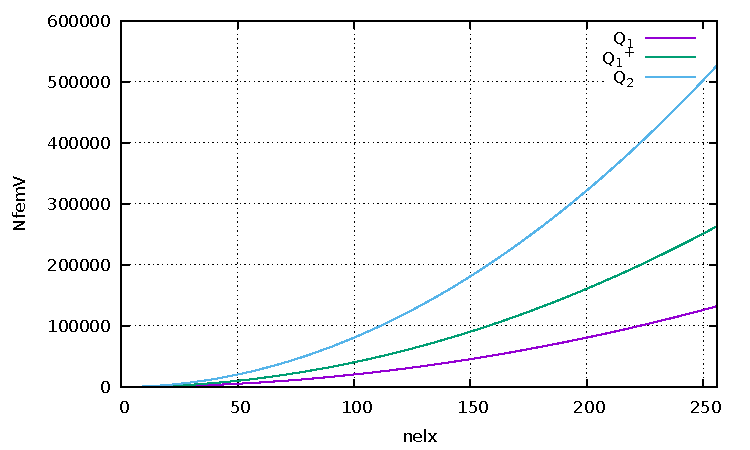
\includegraphics[width=8cm]{images/basis_q1p/NfemV_2D.pdf}
\end{center}




\Literature: 
\begin{itemize}
\item Mons \& Roge (1992) \cite{moro92}, 
\item Li \etal (2009) \cite{lihc09}, 
\item Knobloch \& Tobiska (2000) \cite{knto00}, 
\item Franca \etal (1993) \cite{frha93}, 
\item Idelsohn \etal (1995) \cite{idsn95}.
\end{itemize}



%%%%%%%%%%%%%%%%%%%%%%%%%%%%%%%%%%%%%%%%%%%%%%%%%%%%%%%%%%%%%%%%%%%%%%%%%%%%%%%
\subsection{The rotated $Q_1$ (Rannacher-Turek element)} \label{ss:rq1}
\index{general}{$\tilde{Q}_1$}
\begin{flushright} {\tiny {\color{gray} \tt basis\_q1rc\_2D.tex}} \end{flushright}
%~~~~~~~~~~~~~~~~~~~~~~~~~~~~~~~~~~~~~~~~~~~~~~~~~~~~~~~~~~~~~~~~~~~~~~~~~~~~~~~~~~~~~~~~~~~~~~~~~~

The nodes are not on the corners of the element but in the middle of the
element edges:

\input{tikz/tikz_RTQ1P0}

\begin{verbatim}
+======3======+
|             |
|      s      |
|      |      |
4      +--r   2
|             |
|             |
|             |
+======1======+
\end{verbatim}

There are two types of basis functions: the Middle Point (MP) variant
such that $\bN_i(\vec{r}_j)=\delta_{ij}$ and the Mid Value (MV) variant
such that $\frac{1}{|\Gamma_i|} \int_{\Gamma_i} \bN_j d\Gamma = \delta_{ij}$.

%.............................................
\paragraph{The Middle Point (MP) variant}. 
We have $\tilde{Q}_1=span \{ 1,r,s,r^2-s^2 \}$
so a function $f \in \tilde{Q}_1$  is such that 
\begin{equation}
f(r,s)= a + b r + c s + d(r^2-s^2 )
\label{nonpsf}
\end{equation}
This function must be so that 
\begin{eqnarray}
f_1 &=& f(r=0 ,s=-1) = a -c -d \\
f_2 &=& f(r=+1,s=0)  = a +b +d \\
f_3 &=& f(r=0 ,s=+1) = a +c -d \\
f_4 &=& f(r=-1,s=0)  = a -b +d 
\end{eqnarray}
and then 
\[
\left(
\begin{array}{c}
f_1 \\ f_2 \\ f_3 \\ f_4
\end{array}
\right)
=
\left(
\begin{array}{cccc}
1 &0 &-1 &-1 \\
1 &1 &0 &1 \\
1 &0 &1 &-1 \\
1 &-1 &0 &1
\end{array}
\right)
\cdot
\left(
\begin{array}{c}
a \\ b \\ c \\ d
\end{array}
\right)
\]
This system can easily be solved, and $a,b,c,d$ are then replaced in Eq.~\eqref{nonpsf},
which yields 
\begin{eqnarray}
f(r,s) &=& \bN_1(r,s)f_1 +\bN_2(r,s)f_2 + \bN_3(r,s)f_3 +\bN_4(r,s)f_4
\end{eqnarray}
inside the element with
\begin{mdframed}[backgroundcolor=blue!5]
\begin{eqnarray}
\bN_1(r,s) &=& \frac{1}{4} (1-2s-(r^2-s^2)) \nonumber\\
\bN_2(r,s) &=& \frac{1}{4} (1+2r+(r^2-s^2)) \nonumber\\
\bN_3(r,s) &=& \frac{1}{4} (1+2s-(r^2-s^2)) \nonumber\\
\bN_4(r,s) &=& \frac{1}{4} (1-2r+(r^2-s^2)) \nonumber
\end{eqnarray}
\end{mdframed}
We of course recover the partition of unity property, i.e. $\sum \bN_i(r,s)=1$ for any coordinate $r,s$ inside 
the reference element.

\begin{remark}
These basis functions have been independently proposed by \textcite{dogm81} (1981). The authors
prove herein that this element is checkerboard-free (although they do no show any example
of simulation carried out with this element).
\end{remark}

\begin{eqnarray}
\frac{\partial \bN_1}{\partial r} &=& \frac{1}{2}(-r)\\
\frac{\partial \bN_2}{\partial r} &=& \frac{1}{2}(1+r)\\
\frac{\partial \bN_3}{\partial r} &=& \frac{1}{2}(-r)\\
\frac{\partial \bN_4}{\partial r} &=& \frac{1}{2}(-1+r)
\end{eqnarray}

\begin{eqnarray}
\frac{\partial \bN_1}{\partial s} &=& \frac{1}{2}(-1+s)\\
\frac{\partial \bN_2}{\partial s} &=& \frac{1}{2}(-s)\\
\frac{\partial \bN_3}{\partial s} &=& \frac{1}{2}(1+s)\\
\frac{\partial \bN_4}{\partial s} &=& \frac{1}{2}(-s)
\end{eqnarray}

\begin{center}
\includegraphics[width=6cm]{images/rannacherturek/N1}
\includegraphics[width=6cm]{images/rannacherturek/N2}\\
\includegraphics[width=6cm]{images/rannacherturek/N3}
\includegraphics[width=6cm]{images/rannacherturek/N4}\\
{\captionfont Graphical representation of the $\tilde{Q}_1$ basis functions}
\end{center}

%......................................
\paragraph{The Mid Value (MV) variant}. 

These basis functions are implemented in deal.II
\footnote{\url{https://www.dealii.org/8.5.0/doxygen/deal.II/polynomials_rannacher_turek_8cc_source.html}}
for $x\in[0,1]$ and $y\in[0,1]$:

\begin{eqnarray}
\bN_1(x,y) &=&  0.75 + 1.5x - 2.5y -1.5(x^2-y^2) \quad bottom\\
\bN_2(x,y) &=& -0.25 - 0.5x + 1.5y +1.5(x^2-y^2) \quad right\\
\bN_3(x,y) &=& -0.25 + 1.5x - 0.5y -1.5(x^2-y^2) \quad top\\
\bN_4(x,y) &=&  0.75 - 2.5x + 1.5y +1.5(x^2-y^2) \quad left
\end{eqnarray}
We then proceed to rewrite these for $r\in[-1,1]$ and $t\in[-1:1]$:
\begin{mdframed}[backgroundcolor=blue!5]
\begin{eqnarray}
\bN_1(r,s) &=& \frac{1}{4} -\frac{1}{2}s - \frac{3}{8}(r^2-s^2) \quad bottom \\
\bN_2(r,s) &=& \frac{1}{4} +\frac{1}{2}r + \frac{3}{8}(r^2-s^2) \quad right \\
\bN_3(r,s) &=& \frac{1}{4} +\frac{1}{2}s - \frac{3}{8}(r^2-s^2) \quad top \\
\bN_4(r,s) &=& \frac{1}{4} -\frac{1}{2}r + \frac{3}{8}(r^2-s^2) \quad left
\end{eqnarray}
\end{mdframed}
It is easy to verify that these functions verify the property
\[
\frac{1}{|\Gamma_i|} \int_{\Gamma_i} N_j d\Gamma = \delta_{ij}
\]
These basis functions are used in Shipeng \& Zhongci (2006) \cite{shzh06} 
and mentioned in John \cite[p.722]{john16}.
\begin{eqnarray}
\frac{\partial N_1}{\partial r} &=& -\frac{3}{4}r \nonumber\\
\frac{\partial N_2}{\partial r} &=& \frac{1}{2}+\frac{3}{4}r \nonumber\\
\frac{\partial N_3}{\partial r} &=& -\frac{3}{4}r \nonumber\\
\frac{\partial N_4}{\partial r} &=& -\frac{1}{2}+\frac{3}{4}r \nonumber
\end{eqnarray}

\begin{eqnarray}
\frac{\partial N_1}{\partial t} &=& -\frac{1}{2}+\frac{3}{4}t \nonumber\\
\frac{\partial N_2}{\partial t} &=& -\frac{3}{4}t \nonumber\\
\frac{\partial N_3}{\partial t} &=& \frac{1}{2}+\frac{3}{4}t \nonumber\\
\frac{\partial N_4}{\partial t} &=& -\frac{3}{4}t \nonumber
\end{eqnarray}



%%%%%%%%%%%%%%%%%%%%%%%%%%%%%%%%%%%%%%%%%%%%%%%%%%%%%%%%%%%%%%%%%%%%%%%%%%%%%%%
\subsection{The 2D enriched $Q_1^+\times P_0$ of Fortin} \label{ss:Q1pP02D}

\begin{flushright} {\tiny {\color{gray} \tt basis\_q1fortin\_2D.tex}} \end{flushright}
%~~~~~~~~~~~~~~~~~~~~~~~~~~~~~~~~~~~~~~~~~~~~~~~~~~~~~~~~~~~~~~~~~~~~~~~~~~~~~~~~~~~~~~~~~~~~~~~~~~

We here consider the enriched $Q_1\times P_0$ element introduced first by 
Fortin (1981) \cite{fort81}.
The layout of the degrees of freedom is as follows:

\input{tikz/tikz_q1pp02D}

\noindent The approximation of the velocity components $u$ and $v$ inside the element is
\[
u^h(r,s) = a^u \; \bN_1(r,s) + b^u \;  \bN_2(r,s) + c^u \; \bN_3(r,s) +d^u \; \bN_4(r,s) 
+ d\; b_5^u(r,s) + e\; b_{6}^u(r,s)
\]
\[
v^h(r,s) = a^v \; \bN_1(r,s) + b^v \;  \bN_2(r,s) + c^v \; \bN_3(r,s) +d^v \; \bN_4(r,s) 
+ d^v b_5^v(r,s) + e^v b_{6}^v(r,s)
\]
where $\bN_{1,2,3,4}$ are the standard $Q_1$ basis functions in 2D and with 
\[
b_5^u(r,s) = \frac{1}{2}(1-r)(1-s^2)
\qquad
b_6^u(r,s) = \frac{1}{2}(1+r)(1-s^2)
\]
and
\[
b_5^v(r,s) = \frac{1}{2}(1-r^2)(1-s)
\qquad
b_6^v(r,s) = \frac{1}{2}(1-r^2)(1+s)
\]
In the end one arrives at

\begin{mdframed}[backgroundcolor=blue!5]
\begin{eqnarray}
{\bN}_1^u(r,s) &=&  \bN_1(r,s) - \frac{1}{2} b_5^u(r,s)\nn\\
{\bN}_2^u(r,s) &=&  \bN_2(r,s) - \frac{1}{2} b_6^u(r,s)\nn\\
{\bN}_3^u(r,s) &=&  \bN_3(r,s) - \frac{1}{2} b_6^u(r,s)\nn\\
{\bN}_4^u(r,s) &=&  \bN_4(r,s) - \frac{1}{2} b_5^u(r,s)\nn\\
{\bN}_5^u(r,s) &=&  b_5^u(r,s) \nn\\
{\bN}_6^u(r,s) &=&  b_6^u(r,s) \nn\\
\nn\\
{\bN}_1^v(r,s) &=&  \bN_1(r,s) - \frac{1}{2} b_5^v(r,s)\nn\\
{\bN}_2^v(r,s) &=&  \bN_2(r,s) - \frac{1}{2} b_5^v(r,s)\nn\\
{\bN}_3^v(r,s) &=&  \bN_3(r,s) - \frac{1}{2} b_6^v(r,s)\nn\\
{\bN}_4^v(r,s) &=&  \bN_4(r,s) - \frac{1}{2} b_6^v(r,s)\nn\\
{\bN}_5^v(r,s) &=&  b_5^v(r,s) \nn\\
{\bN}_6^v(r,s) &=&  b_6^v(r,s) 
\end{eqnarray}
\end{mdframed}

We can check for the zero-th order consistency: Let $u(r,s)=C$, then 
\begin{eqnarray}
u^h(r,s) 
= \sum_{i=1}^6 \bN_i^u(r,s) u_i 
= C \sum_{i=1}^6 \bN_i^u(r,s) 
= C \sum_{i=1}^4 \bN_i(r,s)  
= C
\end{eqnarray}








%%%%%%%%%%%%%%%%%%%%%%%%%%%%%%%%%%%%%%%%%%%%%%%%%%%%%%%%%%%%%%%%%%%%%%%%%%%%%%%
\subsection{The $P_1^{NC}$ space} \label{ss:p1nc}
\index{general}{$P_1^{NC}$}
\input{p1nc}



 %-----------
\newpage
\section{Elements and basis functions in 3D} \begin{flushright} {\tiny {\color{gray} elements3D.tex}} \end{flushright}

%%%%%%%%%%%%%%%%%%%%%%%%%%%%%%%%%%%%%%%%%%%%%%%%%%%%%%%%%%%%%%%%%%%%%%%%%%%%%%%
\subsection{Linear basis functions in tetrahedra ($P_1$)}
\index{general}{$P_1$}

\input{basis_p1_3D}

%%%%%%%%%%%%%%%%%%%%%%%%%%%%%%%%%%%%%%%%%%%%%%%%%%%%%%%%%%%%%%%%%%%%%%%%%%%%%%%
\subsection{Enriched linear in tetrahedra($P_1^+$)}
\index{general}{$P_1^+$}

\input{basis_p1p_3D}

%%%%%%%%%%%%%%%%%%%%%%%%%%%%%%%%%%%%%%%%%%%%%%%%%%%%%%%%%%%%%%%%%%%%%%%%%%%%%%%
\subsection{Triquadratic basis functions in 3D ($Q_2$)}
\index{general}{$Q_2$}

\begin{flushright} {\tiny {\color{gray} basis\_q2\_3D.tex}} \end{flushright}
%~~~~~~~~~~~~~~~~~~~~~~~~~~~~~~~~~~~~~~~~~~~~~~~~~~~~~~~~~~~~~~~~~~~~~~~~~~~~~~~~~~~~~~~~~~~~~~~~~~

\begin{center}
\input{tikz/tikz_q2}
\end{center}
Note that the figure above depicts an element in $x,y,z$ space, not the reference
element in $r,s,t$ space which is centered around the origin.

\begin{eqnarray}
\bN_{1} &=& 0.5r(r-1)  \cdot 0.5s(s-1) \cdot 0.5t(t-1) \nn\\
\bN_{2} &=& (1-r^2)    \cdot 0.5s(s-1) \cdot 0.5t(t-1) \nn\\
\bN_{3} &=& 0.5r(r+1)  \cdot 0.5s(s-1) \cdot 0.5t(t-1) \nn\\
\bN_{4} &=&  0.5r(r-1) \cdot (1-s^2)   \cdot 0.5t(t-1) \nn\\
\bN_{5} &=&  (1-r^2)   \cdot (1-s^2)   \cdot 0.5t(t-1) \nn\\
\bN_{6} &=& 0.5r(r+1)  \cdot (1-s^2)   \cdot 0.5t(t-1) \nn\\
\bN_{7} &=&  0.5r(r-1) \cdot 0.5s(s+1) \cdot 0.5t(t-1) \nn\\
\bN_{8} &=&  (1-r^2)   \cdot 0.5s(s+1) \cdot 0.5t(t-1) \nn\\
\bN_{9} &=& 0.5r(r+1)  \cdot 0.5s(s+1) \cdot 0.5t(t-1) \nn\\
\bN_{10}&=&  0.5r(r-1) \cdot 0.5s(s-1) \cdot (1-t^2) \nn\\
\bN_{11}&=&  (1-r^2)   \cdot 0.5s(s-1) \cdot (1-t^2) \nn\\
\bN_{12}&=& 0.5r(r+1)  \cdot 0.5s(s-1) \cdot (1-t^2) \nn\\
\bN_{13}&=&  0.5r(r-1) \cdot (1-s^2)   \cdot (1-t^2) \nn\\
\bN_{14}&=&  (1-r^2)   \cdot (1-s^2)   \cdot (1-t^2) \nn\\
\bN_{15}&=& 0.5r(r+1)  \cdot (1-s^2)   \cdot (1-t^2) \nn\\
\bN_{16}&=&  0.5r(r-1) \cdot 0.5s(s+1) \cdot (1-t^2) \nn\\
\bN_{17}&=&  (1-r^2)   \cdot 0.5s(s+1) \cdot (1-t^2) \nn\\
\bN_{18}&=& 0.5r(r+1)  \cdot 0.5s(s+1) \cdot (1-t^2) \nn\\
\bN_{19}&=&  0.5r(r-1) \cdot 0.5s(s-1) \cdot 0.5t(t+1) \nn\\
\bN_{20}&=&  (1-r^2)   \cdot 0.5s(s-1) \cdot 0.5t(t+1) \nn\\
\bN_{21}&=& 0.5r(r+1)  \cdot 0.5s(s-1) \cdot 0.5t(t+1) \nn\\
\bN_{22}&=&  0.5r(r-1) \cdot (1-s^2)   \cdot 0.5t(t+1) \nn\\
\bN_{23}&=&  (1-r^2)   \cdot (1-s^2)   \cdot 0.5t(t+1) \nn\\
\bN_{24}&=& 0.5r(r+1)  \cdot (1-s^2)   \cdot 0.5t(t+1) \nn\\
\bN_{25}&=&  0.5r(r-1) \cdot 0.5s(s+1) \cdot 0.5t(t+1) \nn\\
\bN_{26}&=&  (1-r^2)   \cdot 0.5s(s+1) \cdot 0.5t(t+1) \nn\\
\bN_{27}&=& 0.5r(r+1)  \cdot 0.5s(s+1) \cdot 0.5t(t+1) \nn
\end{eqnarray}








%%%%%%%%%%%%%%%%%%%%%%%%%%%%%%%%%%%%%%%%%%%%%%%%%%%%%%%%%%%%%%%%%%%%%%%%%%%%%%%
\subsection{Enriched quadratic basis functions in tetrahedra ($P_2^+$)}
\index{general}{$P_2^+$}

\input{basis_p2p_3D}


%%%%%%%%%%%%%%%%%%%%%%%%%%%%%%%%%%%%%%%%%%%%%%%%%%%%%%%%%%%%%%%%%%%%%%%%%%%%%%%
%.....................................................................
\subsection{Linear basis functions for hexahedra ($P_1$)} \label{ss:lbfh3D}
\index{general}{$P_1$}

This is the ${\bm Q}_2\times P_{-1}$ element. 
I choose the reduced coordinates of the pressure nodes to be :

\begin{tabular}{cccc}
\hline
point & r & s & t \\
\hline
1& 1/2 &-1/2 &-1/2\\
2& -1/2 &1/2 &-1/2\\
3& -1/2 &-1/2& 1/2\\
4& 1/2 &1/2& 1/2 \\
\hline
\end{tabular}

Inside the element the pressure is given as a linear function of the reduced coordinates $r,s,t$:
\[
p(r,s,t)=a+br+cs+dt
\]
This expression must exactly interpolate the pressure at all four pressure nodes:
\begin{eqnarray}
p_1 
&=& p(r_1,s_1,t_1) 
= a+br_1+cs_1+dt_1 
= a+b/2-c/2-d/2\nonumber\\
p_2
&=& p(r_2,s_2,t_2)
= a+br_2+cs_2+dt_2
= a-b/2+c/2-d/2\nonumber\\
p_3
&=& p(r_3,s_3,t_3) 
= a+br_3+cs_3+dt_3 
= a-b/2-c/2+d/2\nonumber\\
p_4
&=& p(r_4,s_4,t_4) 
= a+br_4+cs_4+dt_4
= a+b/2+c/2+d/2\nonumber
\end{eqnarray}
or,
\begin{equation}
\left(
\begin{array}{cccc}
1 & 1/2 & -1/2 & -1/2 \\
1 & -1/2 & +1/2 & -1/2 \\
1 & -1/2 & -1/2 & +1/2 \\
1 & 1/2 & +1/2 & +1/2 
\end{array}
\right)
\left(
\begin{array}{c}
a\\b\\c\\d
\end{array}
\right)=
\left(
\begin{array}{c}
p_1\\p_2\\p_3\\p_4
\end{array}
\right)
\nonumber
\end{equation}

The matrix is invertible and we get:
\[
\left(
\begin{array}{c}
a\\b\\c\\d
\end{array}
\right)=
\left(
\begin{array}{cccc}
1/4 & 1/4 & 1/4 & 1/4 \\
1/2 & -1/2 & -1/2 & 1/2 \\
-1/2 & 1/2 & -1/2 & 1/2 \\
-1/2 & -1/2 & 1/2 & 1/2
\end{array}
\right)
\left(
\begin{array}{c}
p_1\\p_2\\p_3\\p_4
\end{array}
\right)
\]

so 
\begin{eqnarray}
p(r,s,t)
&=& a+br+cs+dt \nonumber\\
&=& \frac{1}{4}(p_1+p_2+p_3+p_4)
+\frac{1}{2}(p_1-p_2-p_3+p_4)r
+\frac{1}{2}(-p_1+p_2-p_3+p_4)s
+\frac{1}{2}(-p_1-p_2+p_3+p_4)t\nonumber\\
&=&
\frac{1}{4}(1+2r-2s-2t)p_1+
\frac{1}{4}(1-2r+2s-2t)p_2+
\frac{1}{4}(1-2r-2s+2t)p_3+
\frac{1}{4}(1+2r+2s+2t)p_4 \nonumber\\
&=& \sum_{i=1}^4 N_i(r,s,t) p_i
\end{eqnarray}
with
\begin{eqnarray}
N_1(r,s,t) &=& \frac{1}{4}(1+2r-2s-2t)\nonumber\\
N_2(r,s,t) &=& \frac{1}{4}(1-2r+2s-2t)\nonumber\\
N_3(r,s,t) &=& \frac{1}{4}(1-2r-2s+2t)\nonumber\\
N_4(r,s,t) &=& \frac{1}{4}(1+2r+2s+2t)\nonumber
\end{eqnarray}

\vspace{.6cm}

I could also have chosen 

\begin{tabular}{cccc}
\hline
point & r & s & t \\
\hline
1& 0 & 0 &0 \\
2& 1 & 0 &0 \\
3& 0 & 1 &0 \\
4& 0 & 0 &1 \\
\hline
\end{tabular}

This expression must exactly interpolate the pressure at all four pressure nodes:
\begin{eqnarray}
p_1  &=& p(r_1,s_1,t_1) = a+br_1+cs_1+dt_1 = a\nonumber\\
p_2  &=& p(r_2,s_2,t_2) = a+br_2+cs_2+dt_2 = a+b\nonumber\\
p_3  &=& p(r_3,s_3,t_3) = a+br_3+cs_3+dt_3 = a+c\nonumber\\
p_4  &=& p(r_4,s_4,t_4) = a+br_4+cs_4+dt_4 = a+d\nonumber
\end{eqnarray}
i.e.
\[
a=p_1
\qquad
b=p_2-p1
\qquad
c=p_3-p1
\qquad
d=p_4-p1
\]
or, 
\[
p^h(r,s)=a+br+cs+dt=p_1 + (p_2-p_1)r + (p_3-p_1)r + (p_4-p_1)t  = p_1(1-r-s-t) + r p_2 + s p_3 + t p_4
\]
so 
\begin{mdframed}[backgroundcolor=blue!5]
\begin{eqnarray}
N_1(r,s,t) &=& 1-r-s-t \\ 
N_2(r,s,t) &=& r \\
N_3(r,s,t) &=& s \\
N_4(r,s,t) &=& t
\end{eqnarray}
\end{mdframed}






%%%%%%%%%%%%%%%%%%%%%%%%%%%%%%%%%%%%%%%%%%%%%%%%%%%%%%%%%%%%%%%%%%%%%
\subsection{20-node serendipity basis functions in 3D ($Q_2^{(20)}$)}
\index{general}{$Q_2^{(20)}$} \index{general}{Serendipity element}

The serendipity elements are those rectangular elements which have no
interior nodes \cite[p91]{reddybook2}.

\begin{verbatim}
   t
   |
   .--s
  /
 r
                                    05=====20=====08 
                                    |             |  
                                    |             |  
                  17 - - - - - -19  13            16
                  .              .  |             |  
                  .              .  |             |  
06=====18=====07  .              .  01=====12=====04 @ r=-1
|             |   .              . 
|             |   .              .  
14            15  09 - - - - - -11 @ r=0
|             |   
|             |  
02=====10=====03 @ r=+1
\end{verbatim}

\todo[inline]{find/build basis functions!}


%..........................................................................---------------------------
%\subsection{Enriched linear basis functions in quadrilaterals ($Q_1^+$) -WIP} \label{ss:quadmini3D}
%\index{general}{$Q_1^+$}

%\input{lamichhane3D}


%-----------------------------------------------------------------
\subsection{The rotated $Q_1$} \label{ss:rq1_3D}
\index{general}{$\tilde{Q}_1$}

The nodes are not on the corners of the element but in the middle of the
element faces:

\begin{center}
\includegraphics[width=4cm]{images/rannacherturek/elt3D}\\
{\captionfont Node numbering and connectivity pattern of the reference element. Taken from \cite{gekm08}}
\end{center}

We have $\tilde{Q}_1=span \{1,r,s,t,r^2-s^2,s^2-t^2\}$.

%.............................................
\paragraph{The Middle Point (MP) variant}. 

The basis functions are given by (see Georgiev \etal (2008) \cite{gekm08}):
\begin{eqnarray}
N_1(r,s,t) &=& \frac{1}{6}(1-3r+2r^2-s^2-t^2 ) \\
N_2(r,s,t) &=& \frac{1}{6}(1+3r+2r^2-s^2-t^2 ) \\
N_3(r,s,t) &=& \frac{1}{6}(1-r^2-3s+2s^2-t^2 ) \\
N_4(r,s,t) &=& \frac{1}{6}(1-r^2+3s+2s^2-t^2 ) \\
N_5(r,s,t) &=& \frac{1}{6}(1-r^2-s^2-3t+2t^2 ) \\
N_6(r,s,t) &=& \frac{1}{6}(1-r^2-s^2+3t+2t^2 ) 
\end{eqnarray}

\begin{eqnarray}
\frac{\partial N_1}{\partial r} &=& \frac{1}{6} (-3+4r )\\
\frac{\partial N_2}{\partial r} &=& \frac{1}{6} (3+4r )\\
\frac{\partial N_3}{\partial r} &=& \frac{1}{6} (-2r) \\
\frac{\partial N_4}{\partial r} &=& \frac{1}{6} (-2r) \\
\frac{\partial N_5}{\partial r} &=& \frac{1}{6} (-2r) \\
\frac{\partial N_6}{\partial r} &=& \frac{1}{6} (-2r) 
\end{eqnarray}

\begin{eqnarray}
\frac{\partial N_1}{\partial s} &=& \frac{1}{6} (-2s)\\ 
\frac{\partial N_2}{\partial s} &=& \frac{1}{6} (-2s) \\
\frac{\partial N_3}{\partial s} &=& \frac{1}{6} (-3+4s )\\
\frac{\partial N_4}{\partial s} &=& \frac{1}{6} (3+4s )\\
\frac{\partial N_5}{\partial s} &=& \frac{1}{6} (-2s) \\
\frac{\partial N_6}{\partial s} &=& \frac{1}{6} (-2s) 
\end{eqnarray}

\begin{eqnarray}
\frac{\partial N_1}{\partial t} &=& \frac{1}{6}(-2t) \\ 
\frac{\partial N_2}{\partial t} &=& \frac{1}{6}(-2t) \\ 
\frac{\partial N_3}{\partial t} &=& \frac{1}{6}(-2t) \\ 
\frac{\partial N_4}{\partial t} &=& \frac{1}{6}(-2t) \\ 
\frac{\partial N_5}{\partial t} &=& \frac{1}{6}(-3+4t) \\ 
\frac{\partial N_6}{\partial t} &=& \frac{1}{6}(3+4t)  
\end{eqnarray}


%......................................
\paragraph{The Mid Value (MV) variant}. 

\begin{eqnarray}
N_1(r,s,t) &=& \frac{1}{12}(2-6r+6r^2-3s^2-3t^2) \\
N_2(r,s,t) &=& \frac{1}{12}(2+6r+6r^2-3s^2-3t^2) \\
N_3(r,s,t) &=& \frac{1}{12}(2-3r^2-6s+6s^2-3t^2) \\
N_4(r,s,t) &=& \frac{1}{12}(2-3r^2+6s+6s^2-3t^2) \\
N_5(r,s,t) &=& \frac{1}{12}(2-3r^2-3s^2-6t+6t^2) \\
N_6(r,s,t) &=& \frac{1}{12}(2-3r^2-3s^2+6t+6t^2)
\end{eqnarray}

\begin{eqnarray}
\frac{\partial N_1}{\partial r} &=& \frac{1}{12}(-6+12r) = \frac{1}{2}(-1+2r)\\
\frac{\partial N_2}{\partial r} &=& \frac{1}{12}(6+12r) = \frac{1}{2}(1+2r)\\
\frac{\partial N_3}{\partial r} &=& \frac{1}{12}(-6r) = -\frac{1}{2}r \\
\frac{\partial N_4}{\partial r} &=& \frac{1}{12}(-6r) = -\frac{1}{2}r \\
\frac{\partial N_5}{\partial r} &=& \frac{1}{12}(-6r) = -\frac{1}{2}r \\
\frac{\partial N_6}{\partial r} &=& \frac{1}{12}(-6r) = -\frac{1}{2}r 
\end{eqnarray}

\begin{eqnarray}
\frac{\partial N_1}{\partial s} &=& \frac{1}{12} (-6s) = -\frac{1}{2}s \\
\frac{\partial N_2}{\partial s} &=& \frac{1}{12} (-6s) = -\frac{1}{2}s \\
\frac{\partial N_3}{\partial s} &=& \frac{1}{12} (-6+12s) = \frac{1}{2} (-1+2s) \\ 
\frac{\partial N_4}{\partial s} &=& \frac{1}{12} (6+12s) = \frac{1}{2} (1+2s) \\ 
\frac{\partial N_5}{\partial s} &=& \frac{1}{12} (-6s) = -\frac{1}{2}s \\
\frac{\partial N_6}{\partial s} &=& \frac{1}{12} (-6s) = -\frac{1}{2}s 
\end{eqnarray}

\begin{eqnarray}
\frac{\partial N_1}{\partial t} &=& \frac{1}{12} (-6t) = -\frac{1}{2}t \\
\frac{\partial N_2}{\partial t} &=& \frac{1}{12} (-6t) = -\frac{1}{2}t \\
\frac{\partial N_3}{\partial t} &=& \frac{1}{12} (-6t) = -\frac{1}{2}t \\
\frac{\partial N_4}{\partial t} &=& \frac{1}{12} (-6t) = -\frac{1}{2}t \\
\frac{\partial N_5}{\partial t} &=& \frac{1}{12} (-6+12t) = \frac{1}{2} (-1+2t) \\ 
\frac{\partial N_6}{\partial t} &=& \frac{1}{12} (6+12t) = \frac{1}{2} (1+2t) 
\end{eqnarray}






%-----------------------------------------------------------------------------
\subsection{The 3D enriched $Q_1^+\times P_0$ of Fortin} \label{ss:Q1pP03D}

This element is mentioned on p249 of Cuvelier, Segal \& van Steenhoven \cite{cuss86}:
"The enriched trilinear velocity-constant pressure element is probably the simplest admissible 3D element."
Fortin \cite{fort81} designed a simple LBB-stable $Q_1$ element to which mid-face nodes are added, 
i.e. a 'bubble' $Q_2$ function is added on each face.
However, only $\vec\upnu\cdot \vec{n}$ is present on these mid-face nodes: 

\input{tikz/tikz_q1pp0}

Fortin states: "this element satisfies the B.B. condition and is probably the 
simplest 3-D element to do So. This
unfortunately does not mean that it is more accurate (at least on regular meshes)." and 
"the element satisfies the B.B. condition. It can therefore be used in a non-regular mesh 
without fear. The number of
degrees of freedom is approximately double with respect to the $Q_1\times P_0$ element and this is
reflected by an increased number of vortices and a reduction of their size. However, there
seems to be a qualitative deficiency of these vortices since they do not easily assemble into
complex flows. Only numerical experiments can give the final answer."
This element is mentioned/used in \cite{rota87b,begt92,vadv03}.

Considering a single element, we have 
\begin{itemize}
\item $Q_1$: $2\times 2\times 2\times 3=24$ velocity dofs
\item $Q_1^+$: $2\times 2\times 2\times 3+6 = 30$ velocity dofs: 
\[
\vec{V}^T=(\underbrace{u_1,v_1,w_1,\dots,u_8,v_8,w_8}_{Q_1\; dofs},
\underbrace{u_9,v_9,w_9,u_{10},v_{10},w_{10}}_{bubble \; dofs})
\]
The big difference with all other elements so far is the fact that the 
dofs $u_9,v_9,w_9$ are not colocated (same
for the other three). $u_9$ lives in the middle of the $r=-1$ face, $v_9$ lives in 
the middle of the $s=-1$ face and 
$w_9$ lives in the middle of the $t=-1$ face.

\item $Q_2$: $3\times 3\times 3\times 3=81$ velocity dofs 
\end{itemize}

Considering a 3D mesh composed of $nel=nelx\times nely\times nelz$ elements:
\begin{itemize}
\item $Q_1$: the total number of Velocity dofs is $NfemV=(nelx+1)\times(nely+1)\times(nelz+1)\times 3$
\item $Q_1^+$:  the total number of nodes is 
\[NfemV=(nelx+1)\times(nely+1)\times(nelz+1)\times 3 
+ (nelx+1)\times nely\times nelz
+ nelx\times (nely+1)\times nelz
+ nelx\times nely \times (nelz+1)
\]
\item $Q_2$: the total number of Velocity dofs is 
$NfemV=(2nelx+1)\times (2nely+1)\times (2nelz+1)\times 3$
\end{itemize}

When $nelx=nely=nelz=n>>1$ then the numbers above converge to 
$3n^3$, $6n^3$ and $24n^3$ respectively. This means that for large meshes 
the enriched $Q_1$ uses twice as many dofs as the standard $Q_1$ while the 
$Q_2$ element uses 8 times more. 



\paragraph{$x$-component of velocity} The polynomial representation of the velocity in the element is given by 
\[
u^h(r,s,t) = a + br +c s + d t +e rs + f rt + g st + h rst
+ k b_9(r,s,t) + l b_{10}(r,s,t)
\]
where the two bubble functions are:
\[
b_9^u(r,s,t)=\frac{1}{2}(1-r)(1-s^2)(1-t^2)
\qquad
b_{10}^u(r,s,t)=\frac{1}{2}(1+r)(1-s^2)(1-t^2)
\]
The coordinates of the $u_9$ dof is (-1,0,0) and the coordinate of the $u_{10}$ dof is $(1,0,0)$.
We see that the bubble functions are 1 at their nodes and zero at all other nodes.
We can actually use a different basis for ${1,r,s,t,rs,rt,st,rst}$ and we 
instead choose the standard $Q_1$ functions so that $u^h$ becomes:
\[
u^h(r,s,t) = aN_1 + b N_2 + cN_3 +dN_4 + eN_5 + fN_6 + gN_7 + hN_8 
+ k b_9(r,s,t) + l b_{10}(r,s,t)
\]
We then must find the set of coefficients $\{a \dots l\}$ and we will do so by 
requiring that $u^h(r_i,s_i,t_i)=u_i$ for $i=1,10$. 

The coordinates of all 10 nodes and the values of basis functions at these locations are:

\begin{center}
\begin{tabular}{c|ccc|cccccccc|cc}
\hline
node $\#$  & $r$ & $s$ & $t$ & $N_1$ & $N_2$ & $N_3$ & $N_4$ & $N_5$ & $N_6$ & $N_7$ & $N_8$ & $b_9^u$ & $b_{10}^u$\\
\hline\hline
1 & -1 & -1 & -1 & 1 & 0 & 0 & 0 & 0 & 0 & 0 & 0 & 0 & 0\\
2 & +1 & -1 & -1 & 0 & 1 & 0 & 0 & 0 & 0 & 0 & 0 & 0 & 0\\
3 & +1 & +1 & -1 & 0 & 0 & 1 & 0 & 0 & 0 & 0 & 0 & 0 & 0\\
4 & -1 & +1 & -1 & 0 & 0 & 0 & 1 & 0 & 0 & 0 & 0 & 0 & 0\\
5 & -1 & -1 & +1 & 0 & 0 & 0 & 0 & 1 & 0 & 0 & 0 & 0 & 0\\
6 & +1 & -1 & +1 & 0 & 0 & 0 & 0 & 0 & 1 & 0 & 0 & 0 & 0\\
7 & +1 & +1 & +1 & 0 & 0 & 0 & 0 & 0 & 0 & 1 & 0 & 0 & 0\\
8 & -1 & +1 & +1 & 0 & 0 & 0 & 0 & 0 & 0 & 0 & 1 & 0 & 0\\
9 & -1 & 0 & 0 & 1/4 & 0   & 0 & 1/4 & 1/4& 0   & 0 & 1/4 & 1 & 0\\
10& +1 & 0 & 0 & 0   & 1/4 & 1/4 & 0  &0 & 1/4 & 1/4 & 0 & 0 & 1\\
\hline
\end{tabular}
\end{center}

We then have the following ten equations:
\begin{eqnarray}
u_1=u^h(r_1,s_1,t_1) &=& a \nn \\
u_2=u^h(r_1,s_1,t_1) &=& b \nn \\
u_3=u^h(r_1,s_1,t_1) &=& c \nn \\
u_4=u^h(r_1,s_1,t_1) &=& d \nn \\
u_5=u^h(r_1,s_1,t_1) &=& e \nn \\
u_6=u^h(r_1,s_1,t_1) &=& f \nn \\
u_7=u^h(r_1,s_1,t_1) &=& g \nn \\
u_8=u^h(r_1,s_1,t_1) &=& h \nn \\
u_9=u^h(r_9,s_9,t_9) &=& \frac{1}{4}(a+d+e+h)+k \nn \\
u_{10}=u^h(r_{10},s_{10},t_{10}) &=& \frac{1}{4}(b+c+f+g)+l \nn
\end{eqnarray}
or, 
\[
\left(
\begin{array}{cccccccccc}
 1 & 0 & 0 & 0 & 0 & 0 & 0 & 0 & 0 & 0\\
 0 & 1 & 0 & 0 & 0 & 0 & 0 & 0 & 0 & 0\\
 0 & 0 & 1 & 0 & 0 & 0 & 0 & 0 & 0 & 0\\
 0 & 0 & 0 & 1 & 0 & 0 & 0 & 0 & 0 & 0\\
 0 & 0 & 0 & 0 & 1 & 0 & 0 & 0 & 0 & 0\\
 0 & 0 & 0 & 0 & 0 & 1 & 0 & 0 & 0 & 0\\
 0 & 0 & 0 & 0 & 0 & 0 & 1 & 0 & 0 & 0\\
 0 & 0 & 0 & 0 & 0 & 0 & 0 & 1 & 0 & 0\\
 1/4 & 0   & 0 & 1/4 & 1/4& 0   & 0 & 1/4 & 1 & 0\\
 0   & 1/4 & 1/4 & 0  &0 & 1/4 & 1/4 & 0 & 0 & 1
\end{array}
\right)
\cdot
\left(
\begin{array}{c}
a \\ b\\ c\\ d\\ e\\ f\\ g\\ h\\ k\\ l
\end{array}
\right)
=
\left(
\begin{array}{c}
u_1 \\ u_2 \\ u_3 \\ u_4 \\ u_5 \\ u_6 \\ u_7 \\ u_8 \\ u_9 \\ u_{10}
\end{array}
\right)
\]

This yields
\begin{eqnarray}
a &=& u_1 \nn\\
b &=& u_2 \nn\\
c &=& u_3 \nn\\
d &=& u_4 \nn\\
e &=& u_5 \nn\\
f &=& u_6 \nn\\
g &=& u_7 \nn\\
h &=& u_8 \nn\\
k &=& u_9-\frac{1}{4}(u_1 + u_4 + u_5 + u_8) \nn\\
l &=& u_{10}-\frac{1}{4}(u_2 + u_3 + u_6 + u_7) \nn 
\end{eqnarray}

and then 
\begin{eqnarray}
u^h(r,s,t)  
&=& aN_1 + b N_2 + cN_3 +dN_4 + eN_5 + fN_6 + gN_7 + hN_8 
+ k b_9^u(r,s,t) + l b_{10}^u(r,s,t) \nn\\
&=& u_1N_1 + u_2 N_2 + u_3N_3 +u_4N_4 + u_5N_5 + u_6N_6 + u_7N_7 + u_8N_8 \nn\\
&& +
\left[u_9-\frac{1}{4}(u_1 + u_4 + u_5 + u_8)\right] b_9^u(r,s,t) +
\left[u_{10}-\frac{1}{4}(u_2 + u_3 + u_6 + u_7)\right] b_{10}^u(r,s,t) \nn\\
&=& 
\left(u_1-\frac{1}{4}b_9\right)N_1 +
\left(u_2-\frac{1}{4}b_{10}\right)N_2 +
\left(u_3-\frac{1}{4}b_{10}\right)N_3 +
\left(u_4-\frac{1}{4}b_9\right)N_4 + \nn\\
&&
\left(u_5-\frac{1}{4}b_9\right)N_5 +
\left(u_6-\frac{1}{4}b_{10}\right)N_6 +
\left(u_7-\frac{1}{4}b_{10}\right)N_7 +
\left(u_8-\frac{1}{4}b_9\right)N_8 + \nn\\
&& b_9^u(r,s,t) u_9+  b_{10}^u(r,s,t) u_{10} \nn
\end{eqnarray}

Finally, we can write the basis functions for the $u$ field:

\begin{mdframed}[backgroundcolor=blue!5]
\begin{eqnarray}
{N}_1^u(r,s,t) &=&  N_1(r,s,t) - \frac{1}{4} b_9^u(r,s,t)\nn\\
{N}_2^u(r,s,t) &=&  N_2(r,s,t) - \frac{1}{4} b_{10}^u(r,s,t)\nn\\
{N}_3^u(r,s,t) &=&  N_3(r,s,t) - \frac{1}{4} b_{10}^u(r,s,t)\nn\\
{N}_4^u(r,s,t) &=&  N_4(r,s,t) - \frac{1}{4} b_9^u(r,s,t)\nn\\
{N}_5^u(r,s,t) &=&  N_5(r,s,t) - \frac{1}{4} b_9^u(r,s,t)\nn\\
{N}_6^u(r,s,t) &=&  N_6(r,s,t) - \frac{1}{4} b_{10}^u(r,s,t)\nn\\
{N}_7^u(r,s,t) &=&  N_7(r,s,t) - \frac{1}{4} b_{10}^u(r,s,t)\nn\\
{N}_8^u(r,s,t) &=&  N_8(r,s,t) - \frac{1}{4} b_9^u(r,s,t)\nn\\
{N}_9^u(r,s,t) &=&  b_9^u(r,s,t)\nn\\
{N}_{10}^u(r,s,t) &=&  b_{10}^u(r,s,t) \nn
\end{eqnarray}
\end{mdframed}
And it is easy to verify that  
\[
\sum_{i=1}^{10} {N}_i^u(r,s,t) = 1  \qquad \forall r,s,t
\]
During the implementation phase we will need the derivatives of the basis functions, 
which are trivial for the standard $Q_1$ basis functions $N_i$. Remain then 


\begin{eqnarray}
\partial_r b_9^u(r,s,t) 
&=& \frac{\partial }{\partial r}  \left( \frac{1}{2}(1-r)(1-s^2)(1-t^2) \right) 
=  -\frac{1}{2}(1-s^2)(1-t^2)  \nn\\
\partial_s b_9^u(r,s,t) 
&=& \frac{\partial }{\partial s}  \left( \frac{1}{2}(1-r)(1-s^2)(1-t^2) \right) 
=  -(1-r)s(1-t^2)  \nn\\
\partial_t b_9^u(r,s,t) 
&=& \frac{\partial }{\partial t}  \left( \frac{1}{2}(1-r)(1-s^2)(1-t^2) \right) 
=  -(1-r)(1-s^2)t  \nn\\ \nn\\
\partial_r b_{10}^u(r,s,t) 
&=& \frac{\partial }{\partial r}  \left( \frac{1}{2}(1+r)(1-s^2)(1-t^2) \right) 
=  \frac{1}{2}(1-s^2)(1-t^2)  \nn\\
\partial_s b_{10}^u(r,s,t) 
&=& \frac{\partial }{\partial s}  \left( \frac{1}{2}(1+r)(1-s^2)(1-t^2) \right) 
=  -(1+r)s(1-t^2)  \nn\\
\partial_t b_{10}^u(r,s,t) 
&=& \frac{\partial }{\partial t}  \left( \frac{1}{2}(1+r)(1-s^2)(1-t^2) \right) 
=  -(1+r)(1-s^2)t  \nn
\end{eqnarray}

%.........................................
\paragraph{$y$-component of velocity} 
The bubbles are given by 
\[
b_9^v(r,s,t)=\frac{1}{2}(1-r^2)(1-s)(1-t^2)
\qquad
b_{10}^v(r,s,t)=\frac{1}{2}(1-r^2)(1+s)(1-t^2)
\]
The coordinates of all 10 nodes and the values of basis functions at these locations are:
\begin{center}
\begin{tabular}{c|ccc|cccccccc|cc}
\hline
node $\#$  & $r$ & $s$ & $t$ & $N_1$ & $N_2$ & $N_3$ & $N_4$ & $N_5$ & $N_6$ & $N_7$ & $N_8$ & $b_9^v$ & $b_{10}^v$\\
\hline\hline
1 & -1 & -1 & -1 & 1 & 0 & 0 & 0 & 0 & 0 & 0 & 0 & 0 & 0\\
2 & +1 & -1 & -1 & 0 & 1 & 0 & 0 & 0 & 0 & 0 & 0 & 0 & 0\\
3 & +1 & +1 & -1 & 0 & 0 & 1 & 0 & 0 & 0 & 0 & 0 & 0 & 0\\
4 & -1 & +1 & -1 & 0 & 0 & 0 & 1 & 0 & 0 & 0 & 0 & 0 & 0\\
5 & -1 & -1 & +1 & 0 & 0 & 0 & 0 & 1 & 0 & 0 & 0 & 0 & 0\\
6 & +1 & -1 & +1 & 0 & 0 & 0 & 0 & 0 & 1 & 0 & 0 & 0 & 0\\
7 & +1 & +1 & +1 & 0 & 0 & 0 & 0 & 0 & 0 & 1 & 0 & 0 & 0\\
8 & -1 & +1 & +1 & 0 & 0 & 0 & 0 & 0 & 0 & 0 & 1 & 0 & 0\\
9 &  0 & -1 &  0 & 1/4 & 1/4 & 0 & 0 & 1/4 & 1/4 & 0 & 0 & 1& 0\\
10&  0 & +1 &  0 & 0 & 0 & 1/4 & 1/4 & 0 & 0 & 1/4 & 1/4 & 0& 1\\
\hline
\end{tabular}
\end{center}

Then

\begin{mdframed}[backgroundcolor=blue!5]
\begin{eqnarray}
{N}_1^v(r,s,t) &=&  N_1(r,s,t) - \frac{1}{4} b_9^v(r,s,t)\nn\\
{N}_2^v(r,s,t) &=&  N_2(r,s,t) - \frac{1}{4} b_9^v(r,s,t)\nn\\
{N}_3^v(r,s,t) &=&  N_3(r,s,t) - \frac{1}{4} b_{10}^v(r,s,t)\nn\\
{N}_4^v(r,s,t) &=&  N_4(r,s,t) - \frac{1}{4} b_{10}^v(r,s,t)\nn\\
{N}_5^v(r,s,t) &=&  N_5(r,s,t) - \frac{1}{4} b_9^v(r,s,t)\nn\\
{N}_6^v(r,s,t) &=&  N_6(r,s,t) - \frac{1}{4} b_9^v(r,s,t)\nn\\
{N}_7^v(r,s,t) &=&  N_7(r,s,t) - \frac{1}{4} b_{10}^v(r,s,t)\nn\\
{N}_8^v(r,s,t) &=&  N_8(r,s,t) - \frac{1}{4} b_{10}^v(r,s,t)\nn\\
{N}_9^v(r,s,t) &=&  b_9^v(r,s,t)\nn\\
{N}_{10}^v(r,s,t) &=&  b_{10}^v(r,s,t)
\end{eqnarray}
\end{mdframed}

%.........................................
\paragraph{$z$-component of velocity} 



The bubbles are given by 
\[
b_9^w(r,s,t)=\frac{1}{2}(1-r^2)(1-s^2)(1-t)
\qquad
b_{10}^w(r,s,t)=\frac{1}{2}(1-r^2)(1-s^2)(1+t)
\]
The coordinates of all 10 nodes and the values of basis functions at these locations are:
\begin{center}
\begin{tabular}{c|ccc|cccccccc|cc}
\hline
node $\#$  & $r$ & $s$ & $t$ & $N_1$ & $N_2$ & $N_3$ & $N_4$ & $N_5$ & $N_6$ & $N_7$ & $N_8$ & $b_9^w$ & $b_{10}^w$\\
\hline\hline
1 & -1 & -1 & -1 & 1 & 0 & 0 & 0 & 0 & 0 & 0 & 0 & 0 & 0\\
2 & +1 & -1 & -1 & 0 & 1 & 0 & 0 & 0 & 0 & 0 & 0 & 0 & 0\\
3 & +1 & +1 & -1 & 0 & 0 & 1 & 0 & 0 & 0 & 0 & 0 & 0 & 0\\
4 & -1 & +1 & -1 & 0 & 0 & 0 & 1 & 0 & 0 & 0 & 0 & 0 & 0\\
5 & -1 & -1 & +1 & 0 & 0 & 0 & 0 & 1 & 0 & 0 & 0 & 0 & 0\\
6 & +1 & -1 & +1 & 0 & 0 & 0 & 0 & 0 & 1 & 0 & 0 & 0 & 0\\
7 & +1 & +1 & +1 & 0 & 0 & 0 & 0 & 0 & 0 & 1 & 0 & 0 & 0\\
8 & -1 & +1 & +1 & 0 & 0 & 0 & 0 & 0 & 0 & 0 & 1 & 0 & 0\\
9 &  0 &  0 & -1 & 1/4 & 1/4 & 1/4 & 1/4 & 0 & 0 & 0 & 0&  1& 0\\
10&  0 &  0 & +1 & 0 & 0 &0 & 0 & 1/4 & 1/4  & 1/4 & 1/4 & 0& 1\\
\hline
\end{tabular}
\end{center}


\begin{mdframed}[backgroundcolor=blue!5]
\begin{eqnarray}
{N}_1^w(r,s,t) &=&  N_1(r,s,t) - \frac{1}{4} b_9^w(r,s,t)\nn\\
{N}_2^w(r,s,t) &=&  N_2(r,s,t) - \frac{1}{4} b_9^w(r,s,t)\nn\\
{N}_3^w(r,s,t) &=&  N_3(r,s,t) - \frac{1}{4} b_9^w(r,s,t)\nn\\
{N}_4^w(r,s,t) &=&  N_4(r,s,t) - \frac{1}{4} b_9^w(r,s,t)\nn\\
{N}_5^w(r,s,t) &=&  N_5(r,s,t) - \frac{1}{4} b_{10}^w(r,s,t)\nn\\
{N}_6^w(r,s,t) &=&  N_6(r,s,t) - \frac{1}{4} b_{10}^w(r,s,t)\nn\\
{N}_7^w(r,s,t) &=&  N_7(r,s,t) - \frac{1}{4} b_{10}^w(r,s,t)\nn\\
{N}_8^w(r,s,t) &=&  N_8(r,s,t) - \frac{1}{4} b_{10}^w(r,s,t)\nn\\
{N}_9^w(r,s,t) &=&  b_9^w(r,s,t)\nn\\
{N}_{10}^w(r,s,t) &=&  b_{10}^w(r,s,t) \nn
\end{eqnarray}
\end{mdframed}


%.............................................. 
\paragraph{A word about the ${\bm B}$ matrix} We have  
\begin{eqnarray}
u^h(r,s,t) = \sum_{i=1}^{10} N_i^u(r,s,t) u_i \\
v^h(r,s,t) = \sum_{i=1}^{10} N_i^v(r,s,t) v_i \\
w^h(r,s,t) = \sum_{i=1}^{10} N_i^w(r,s,t) w_i 
\end{eqnarray}

Normally we do not make a distinction between the basis functions 
associated to $u,v,w$ but because of the bubbles on the faces we now have to. 

We have previously established that the strain rate 
vector $\vec{\dot \varepsilon}$ is: 
\begin{equation}
\vec{\dot\varepsilon}=
\left(
\begin{array}{c}
\frac{\partial u}{\partial x} \\ \\
\frac{\partial v}{\partial y} \\ \\
\frac{\partial w}{\partial z} \\ \\
\frac{\partial u}{\partial y}\! +\! \frac{\partial v}{\partial x} \\ \\
\frac{\partial u}{\partial z}\! +\! \frac{\partial w}{\partial x} \\ \\
\frac{\partial v}{\partial z}\! +\! \frac{\partial w}{\partial y} 
\end{array}
\right)
=
\left(
\begin{array}{c}
\sum\limits_i \frac{\partial N_i^u}{\partial x} u_i \\ \\
\sum\limits_i \frac{\partial N_i^v}{\partial y} v_i \\ \\
\sum\limits_i \frac{\partial N_i^w}{\partial z} w_i \\ \\
\sum\limits_i (\frac{\partial N_i^u}{\partial y} u_i\! +\! \frac{\partial N_i^v}{\partial x} v_i) \\ \\
\sum\limits_i (\frac{\partial N_i^u}{\partial z} u_i\! +\! \frac{\partial N_i^w}{\partial x} w_i) \\ \\
\sum\limits_i (\frac{\partial N_i^v}{\partial z} v_i\! +\! \frac{\partial N_i^w}{\partial y} w_i) 
\end{array}
\right)
=
\underbrace{
\left(
\begin{array}{ccccccccccc}
\frac{\partial N_1^u}{\partial x} & 0 & 0 &  \cdots  & \frac{\partial N_{10}^u}{\partial x} & 0 & 0 \\ \\
0 & \frac{\partial N_1^v}{\partial y} & 0 & \cdots & 0 & \frac{\partial N_{10}^v}{\partial y} & 0 \\ \\
0 & 0 & \frac{\partial N_1^w}{\partial z} & \cdots & 0 & 0 & \frac{\partial N_{10}^w}{\partial z}
\\ \\
\frac{\partial N_1^u}{\partial y} &  \frac{\partial N_1^v}{\partial x} &  
0 & \cdots  &\frac{\partial N_{10}^u}{\partial x} 
& \frac{\partial N_{10}^v}{\partial x} & 0 \\ \\
\frac{\partial N_1^u}{\partial z} & 0 & \frac{\partial N_1^w}{\partial x} & \cdots &
\frac{\partial N_{10}^u}{\partial z} & 0 & \frac{\partial N_{m_v}^w}{\partial x} \\  \\
0 &  \frac{\partial N_1^v}{\partial z}  & \frac{\partial N_1^w}{\partial y} & \cdots &
0 &  \frac{\partial N_{10}^v}{\partial z}  & \frac{\partial N_{10}^w}{\partial y} 
\end{array}
\right) 
}_{\bm B}
\!
\cdot
\!
\underbrace{
\left(
\begin{array}{c}
u_1 \\ v_1 \\ w_1 \\ u_2 \\ v_2 \\ w_2 \\ u_3 \\ v_3 \\ \dots \\ u_{10} \\ v_{10} \\ w_{10}
\end{array}
\right)
}_{\vec V} \nn
\end{equation}

\newpage
%-----------------------------------------------------------------------------
\subsection{The $Q_1^{++} \times Q_1$ of Karabelas et al (2020)} \label{ss:Q1Q1bb_3D}

\begin{flushright} {\tiny {\color{gray} \tt q1q13D\_2bubbles.tex}} \end{flushright}
%------------------------------------------------------------------------------

This element is implemented in \stone 82.
The two bubble functions are given in Karabelas \etal (2020) \cite{kahp20}:
\begin{eqnarray}
b_9(r,s,t) &=& \left(\frac{27}{32}\right)^3 (1-r^2)(1-s^2)(1-t^2) \cdot (1-r)(1-s)(1-t) 
= \beta_9(r)\cdot\beta_9(s) \cdot \beta_9(t) \nonumber\\
b_{10}(r,s,t) &=& \left(\frac{27}{32}\right)^3 (1-r^2)(1-s^2)(1-t^2) \cdot (1+r)(1+s)(1+t) 
= \beta_{10}(r)\cdot\beta_{10}(s) \cdot \beta_{10}(t)  \nonumber
\end{eqnarray}
where I have chosen nodes 1 ($\vec{r}_1=(-1,-1,-1)$) and 7 ($\vec{r}_7=(+1,+1,+1)$) 
as diagonally opposed nodes (a requirement from the paper), 
and with
\[
\beta_9(x)=\frac{27}{32} (1-x^2) (1-x)
\qquad
\beta_{10}(x)=\frac{27}{32} (1-x^2) (1+x)
\]

I have added the $(27/32)^3$ coefficients so that these functions are exactly 1 a their 
corresponding nodes.
The term $(1-r^2)(1-s^2)(1-t^2)$ makes sure that the two bubbles are conforming and exactly zero 
on the 6 faces of the element.
In what follows $\tilde{\bN}_{1..8}$ are the standard $Q_1$ basis functions.

\begin{center}
\includegraphics[width=8cm]{images/MINI3D/bubbles.pdf}\\
{\captionfont Representation of bubbles $\beta_9(x)$ and $\beta_{10}(x)$}
\end{center}

\begin{remark}
Bubble function 9 is not zero at node 10 and vice versa!
\end{remark}

The authors state: "This also allows for a straightforward inclusion in combination 
with existing finite element codes since all required
implementations are purely on the element level". This is especially true 
if static condensation is used (the authors explain static condensation 
for the bubbles in the appendix of the paper).

The ten nodes are the standard 8 corners of the $Q_1$ element as well  
as $\vec{r}_9=(-1/3,-1/3,-1/3)$ for $b_9$ and 
$\vec{r}_{10}=(1/3,1/3,1/3)$ for $b_{10}$.
We have the following approximation of function $f$ inside the element:
\[
f^h(r,s,t) = \sum_{i=1}^{8} a_i \tilde{\bN}_i(r,s,t) + a_9 b_9(r,s,t) + a_{10} b_{10}(r,s,t)
\]
We notice that bubble functions are exactly zero at the corners of the reference element and
we can compute the values of the ten polynomials ($\tilde{N}_{1-8}(r,s,t),b_9(r,s,t),b_{10}(r,s,t)$) 
at the ten nodes:
\[
\begin{array}{c|cccccccccc}
 & \tilde{\bN}_1 & \tilde{\bN}_2 & \tilde{\bN}_3 & \tilde{\bN}_4 & \tilde{\bN}_5 
 & \tilde{\bN}_6 & \tilde{\bN}_7 & \tilde{\bN}_8 & b_9 & b_{10}\\
 \hline\hline
\vec{r}_1=(-1,-1,-1)    &1 &0 &0 &0 &0 &0 &0 &0 &0 &0 \\
\vec{r}_2=(+1,-1,-1)    &0 &1 &0 &0 &0 &0 &0 &0 &0 &0 \\
\vec{r}_3=(+1,+1,-1)    &0 &0 &1 &0 &0 &0 &0 &0 &0 &0 \\
\vec{r}_4=(-1,+1,-1)    &0 &0 &0 &1 &0 &0 &0 &0 &0 &0 \\
\vec{r}_5=(-1,-1,+1)    &0 &0 &0 &0 &1 &0 &0 &0 &0 &0 \\
\vec{r}_6=(+1,-1,+1)    &0 &0 &0 &0 &0 &1 &0 &0 &0 &0 \\
\vec{r}_7=(+1,+1,+1)    &0 &0 &0 &0 &0 &0 &1 &0 &0 &0 \\
\vec{r}_8=(-1,+1,+1)    &0 &0 &0 &0 &0 &0 &0 &1 &0 &0 \\
\vec{r}_9=(-\frac13,-\frac13,-\frac13)    &8/27 & 4/27 & 2/27  & 4/27 & 4/27 & 2/27& 1/27& 2/27 &1 & 1/8\\
\vec{r}_{10}=(+\frac13,+\frac13,+\frac13) &1/27 & 2/17 & 4/27 & 2/27 & 2/27& 4/27& 8/27& 4/27& 1/8  &1 \\
\end{array}
\]




We then require that the polynomial representation of $f^h$ of $f$ inside the element
is such that $f^h(\vec{r}_i)=f_i$, i.e.:
\begin{eqnarray}
f_1 = f^h(r_1,s_1,t_1) &=& a_1  \nonumber\\
f_2 = f^h(r_2,s_1,t_1) &=& a_2  \nonumber\\
f_3 = f^h(r_3,s_1,t_1) &=& a_3  \nonumber\\
f_4 = f^h(r_4,s_1,t_1) &=& a_4  \nonumber\\
f_5 = f^h(r_5,s_1,t_1) &=& a_5  \nonumber\\
f_6 = f^h(r_6,s_1,t_1) &=& a_6  \nonumber\\
f_7 = f^h(r_7,s_1,t_1) &=& a_7  \nonumber\\
f_8 = f^h(r_8,s_1,t_1) &=& a_8  \nonumber\\
f_9 = f^h(r_9,s_9,t_9) &=&  \frac{1}{27} (8a_1 + 4a_2 + 2a_3 +4a_4 + 4a_5 + 2a_6 + a_7 +2a_8)  + a_9 + a_{10}/8 
\nonumber\\
f_{10} = f^h(r_{10},s_{10},t_{10}) &=& \frac{1}{27} (a_1 + 2a_2 + 4a_3 +2a_4 + 2a_5 + 4a_6 + 8a_7 +4a_8)  + a_9/8 + a_{10} \nonumber
\end{eqnarray}
or,
\[
\left(
\begin{array}{cccccccccc}
1 &0 &0 &0 &0 &0 &0 &0 &0 &0 \\
0 &1 &0 &0 &0 &0 &0 &0 &0 &0 \\
0 &0 &1 &0 &0 &0 &0 &0 &0 &0 \\
0 &0 &0 &1 &0 &0 &0 &0 &0 &0 \\
0 &0 &0 &0 &1 &0 &0 &0 &0 &0 \\
0 &0 &0 &0 &0 &1 &0 &0 &0 &0 \\
0 &0 &0 &0 &0 &0 &1 &0 &0 &0 \\
0 &0 &0 &0 &0 &0 &0 &1 &0 &0 \\
8/27 & 4/27 & 2/27  & 4/27 & 4/27 & 2/27& 1/27& 2/27 &1 & 1/8\\
1/27 & 2/17 & 4/27 & 2/27 & 2/27& 4/27& 8/27& 4/27& 1/8  &1 
\end{array}
\right)
\cdot
\left(
\begin{array}{c}
a_1 \\ a_2 \\ a_3 \\ a_4 \\ a_5 \\ a_6 \\ a_7 \\ a_8 \\ a_9 \\ a_{10}
\end{array}
\right)
=
\left(
\begin{array}{c}
f_1 \\ f_2 \\ f_3 \\ f_4 \\ f_5 \\ f_6 \\ f_7 \\ f_8 \\ f_9 \\ f_{10}
\end{array}
\right)
\]
which yields $a_i=f_i$ for $i=1,...8$ and 
\begin{eqnarray}
a_9 + a_{10}/8 &=& f_9\underbrace{-\frac{1}{27} (8f_1 + 4f_2 + 2f_3 +4f_4 + 4f_5 + 2f_6 + f_7 +2f_8)}_{\tilde{f}_9}   
\nonumber\\
a_9/8 + a_{10} &=& f_{10}
\underbrace{-\frac{1}{27} (f_1 + 2f_2 + 4f_3 +2f_4 + 2f_5 + 4f_6 + 8f_7 +4f_8)}_{\tilde{f}_{10}} 
\nonumber
\end{eqnarray}

\begin{eqnarray}
8a_9 + a_{10} &=& 8f_9 + 8\tilde{f}_9  \nonumber\\
a_9 + 8a_{10} &=& 8f_{10} +8\tilde{f}_{10}
\nonumber
\end{eqnarray}
and then 
\begin{eqnarray}
a_{9}
&=&\frac{1}{63}(64 {f}_{9}-8{f}_{10}) + \frac{1}{63}(64 \tilde{f}_{9}-8\tilde{f}_{10}) \nonumber\\
&=& \frac{8}{63}(8{f}_{9}-{f}_{10})+\frac{8}{63}(8\tilde{f}_{9}-\tilde{f}_{10}) \nonumber\\
&=& \frac{8}{63}(8{f}_{9}-{f}_{10}) -\frac{1}{27}\frac{8}{63}
\left[ 8 (8f_1 + 4f_2 + 2f_3 +4f_4 + 4f_5 + 2f_6 + f_7 +2f_8) \right. \nonumber\\
&& \left. - (f_1 + 2f_2 + 4f_3 +2f_4 + 2f_5 + 4f_6 + 8f_7 +4f_8) \right] \nonumber\\
&=& \frac{8}{63}(8{f}_{9}-{f}_{10}) -\frac{1}{27}\frac{8}{63} 
( 63 f_1 +30 f_2 +12 f_3  +30f_4 +30f_5 +12f_6 +12f_8)\nonumber\\ \nonumber \\
a_{10} 
&=& \frac{1}{63}(64 {f}_{10}-8{f}_9) + \frac{1}{63}(64 \tilde{f}_{10}-8\tilde{f}_9) \nonumber\\
&=& \frac{8}{63}(8 {f}_{10}-{f}_9) + \frac{8}{63}(8 \tilde{f}_{10}-\tilde{f}_9) \nonumber\\
&=& \frac{8}{63}(8 {f}_{10}-{f}_9) -\frac{1}{27}\frac{8}{63} \left[
8(f_1 + 2f_2 + 4f_3 +2f_4 + 2f_5 + 4f_6 + 8f_7 +4f_8) \right. \nonumber\\
&& \left. -(8f_1 + 4f_2 + 2f_3 +4f_4 + 4f_5 + 2f_6 + f_7 +2f_8)
\right] \nonumber\\
&=&\frac{8}{63}(8 {f}_{10}-{f}_9) -\frac{1}{27}\frac{8}{63} 
(12f_2 + 30f_3 + 12f_4 +12f_5 + 30f_6 + 63f_7 +30f_8      ) \nonumber
\end{eqnarray}

We can then write

\begin{eqnarray}
f^h(r,s,t) 
&=& f_1 \bN_1(r,s,t) + f_2 \bN_2(r,s,t) + f_3 \bN_3(r,s,t) + f_4 \bN_4(r,s,t) \nonumber\\
&+& f_5 \bN_5(r,s,t) + f_6 \bN_6(r,s,t) + f_7 \bN_7(r,s,t) + f_8 \bN_8(r,s,t) \nonumber\\
&+& \left[\frac{8}{63}(8{f}_{9}-{f}_{10})-\frac{1}{27}\frac{8}{63}  ( 63 f_1 +30 f_2 +12 f_3  +30f_4 +30f_5 +12f_6 +12f_8) \right] b_9(r,s,t) \nonumber\\
&&\left[ \frac{8}{63}(8 {f}_{10}-{f}_9)  -\frac{1}{27}\frac{8}{63} (12f_2 + 30f_3 + 12f_4 +12f_5 + 30f_6 + 63f_7 +30f_8) \right] b_{10}(r,s,t) \nonumber\\
%&=& \left(N_1(r,s,t) - \frac{8}{27}b_9(r,s,t) \right) f_1 \nonumber\\
%&+& \left(N_2(r,s,t) - \frac{30}{27}\frac{8}{63} b_9(r,s,t) - \frac{12}{27}\frac{8}{63} b_{10}(r,s,t)  \right) f_2 \nonumber\\
%&+&\left( N_3(r,s,t)  -\frac{12}{27}\frac{8}{63} b_9r,s,t) -\frac{30}{27}\frac{8}{63} b_{10}(r,s,t)  \right)f_3 \nonumber\\
%&+& \left( N_4(r,s,t) -\frac{30}{27}\frac{8}{63} b_{9}r,s,t) -\frac{12}{27}\frac{8}{63} b_{10}r,s,t)\right)f_4 \nonumber\\ 
%&+&\left( N_5(r,s,t)- \frac{30}{27}\frac{8}{63} b_{9}r,s,t) -\frac{12}{27}\frac{8}{63} b_{10}r,s,t) \right) f_5 \nonumber\\
%&+&\left( N_6(r,s,t) -\frac{12}{27}\frac{8}{63} b_9r,s,t) -\frac{30}{27}\frac{8}{63} b_{10}r,s,t) \right) f_6 \nonumber\\
%&+&\left( N_7(r,s,t) - \frac{8}{27}b_{10}(r,s,t) \right) f_7 \nonumber\\
%&+&\left(N_8(r,s,t) -\frac{12}{27}\frac{8}{63} b_9(r,s,t) -\frac{30}{27}\frac{8}{63} b_{10}(r,s,t) \right) f_8 \nonumber\\
%&+& \left(  \frac{64}{63}b_9(r,s,t) -\frac{8}{63} b_{10}(r,s,t) \right) f_9 
%+ \left( -\frac{8}{63} b_{9}(r,s,t)  + \frac{64}{63}b_{10}(r,s,t) \right) f_{10} \nonumber\\
&=& \left(\bN_1(r,s,t) - \frac{2^3}{3^3}b_9(r,s,t) \right) f_1 \nonumber\\
&+& \left(\bN_2(r,s,t) - \frac{2^3}{3^3}\frac{10}{21} b_9(r,s,t) - \frac{2^3}{3^3}\frac{4}{21} b_{10}(r,s,t)  \right) f_2 \nonumber\\
&+&\left( \bN_3(r,s,t)  -\frac{2^3}{3^3}\frac{4}{21} b_9r,s,t) -\frac{2^3}{3^3}\frac{10}{21} b_{10}(r,s,t)  \right)f_3 \nonumber\\
&+& \left( \bN_4(r,s,t) -\frac{2^3}{3^3}\frac{10}{21} b_{9}r,s,t) -\frac{2^3}{3^3}\frac{4}{21} b_{10}(r,s,t)\right)f_4 \nonumber\\ 
&+&\left( \bN_5(r,s,t)- \frac{2^3}{3^3}\frac{10}{21} b_{9}r,s,t) -\frac{2^3}{3^3}\frac{4}{21} b_{10}(r,s,t) \right) f_5 \nonumber\\
&+&\left( \bN_6(r,s,t) -\frac{2^3}{3^3}\frac{4}{21} b_9(r,s,t) -\frac{2^3}{3^3}\frac{10}{21} b_{10}(r,s,t) \right) f_6 \nonumber\\
&+&\left( \bN_7(r,s,t) - \frac{2^3}{3^3}b_{10}(r,s,t) \right) f_7 \nonumber\\
&+&\left( \bN_8(r,s,t) -\frac{2^3}{3^3}\frac{4}{21} b_9(r,s,t) -\frac{2^3}{3^3}\frac{10}{21} b_{10}(r,s,t) \right) f_8 \nonumber\\
&+& \left(  \frac{64}{63}b_9(r,s,t) -\frac{8}{63} b_{10}(r,s,t) \right) f_9 
+ \left( -\frac{8}{63} b_{9}(r,s,t)  + \frac{64}{63}b_{10}(r,s,t) \right) f_{10} 
\end{eqnarray}

and finally arrive at the basis functions:
\begin{mdframed}[backgroundcolor=blue!5]
\begin{eqnarray}
\bN_1(r,s,t)    &=&  \tilde{\bN}_1(r,s,t) - \frac{2^3}{3^3}b_9(r,s,t)      \nonumber\\
\bN_2(r,s,t)    &=&  \tilde{\bN}_2(r,s,t) - \frac{2^3}{3^3}\frac{10}{21} b_9(r,s,t) - \frac{2^3}{3^3}\frac{4}{21} b_{10}(r,s,t)      \nonumber\\
\bN_3(r,s,t)    &=&  \tilde{\bN}_3(r,s,t)  -\frac{2^3}{3^3}\frac{4}{21} b_9(r,s,t) -\frac{2^3}{3^3}\frac{10}{21} b_{10}(r,s,t)      \nonumber\\
\bN_4(r,s,t)    &=&  \tilde{\bN}_4(r,s,t) -\frac{2^3}{3^3}\frac{10}{21} b_{9}(r,s,t) -\frac{2^3}{3^3}\frac{4}{21} b_{10}r,s,t)      \nonumber\\
\bN_5(r,s,t)    &=&  \tilde{\bN}_5(r,s,t)- \frac{2^3}{3^3}\frac{10}{21} b_{9}(r,s,t) -\frac{2^3}{3^3}\frac{4}{21} b_{10}(r,s,t)      \nonumber\\
\bN_6(r,s,t)    &=&  \tilde{\bN}_6(r,s,t) -\frac{2^3}{3^3}\frac{4}{21} b_9(r,s,t) -\frac{2^3}{3^3}\frac{10}{21} b_{10}(r,s,t)      \nonumber\\
\bN_7(r,s,t)    &=&  \tilde{\bN}_7(r,s,t) - \frac{2^3}{3^3}b_{10}(r,s,t)      \nonumber\\
\bN_8(r,s,t)    &=&  \tilde{\bN}_8(r,s,t) -\frac{2^3}{3^3}\frac{4}{21} b_9(r,s,t) -\frac{2^3}{3^3}\frac{10}{21} b_{10}(r,s,t)      \nonumber\\
\bN_9(r,s,t)    &=&  \frac{64}{63}b_9(r,s,t) -\frac{8}{63} b_{10}(r,s,t)      \nonumber\\
\bN_{10}(r,s,t) &=&  -\frac{8}{63} b_{9}(r,s,t)  + \frac{64}{63}b_{10}(r,s,t)       \nonumber
\end{eqnarray}
\end{mdframed}

These are somewhat complex forms for the basis functions so we wish to verify the simple property $\sum \bN_i(r,s,t) =1$ 
for all $(r,s,t)$ inside the element:
\begin{eqnarray}
\sum_{i=1}^{10} \bN_i(r,s,t)  
&=& \sum_{i=1}^{8} \tilde{\bN}_i(r,s,t) \nonumber\\
&+& \left[\frac{2^3}{3^3} \left(-1 -\frac{10}{21} -\frac{4}{21} -\frac{10}{21} -\frac{10}{21} -\frac{4}{21} -\frac{4}{21}\right) + \frac{64}{63} -\frac{8}{63} \right] b_9(r,s,t) \nonumber\\
&+& \left[\frac{2^3}{3^3} \left(-\frac{4}{21} -\frac{10}{21} -\frac{4}{21} -\frac{4}{21} -\frac{10}{21} -1 -\frac{10}{21} \right) -\frac{8}{63} + \frac{64}{63} \right] b_{10}(r,s,t) \nonumber\\
&=& 1 + \left[\frac{2^3}{3^3} (-1 -42/21) +\frac{56}{63}  \right] b_9(r,s,t) 
+ \left[\frac{2^3}{3^3} (-42/21 -1)  + \frac{56}{63} \right] b_{10}(r,s,t) \nonumber\\
&=& 1 + \left[\frac{2^3}{3^3} (-3) + \frac{8}{9} \right] b_9(r,s,t) 
+ \left[\frac{2^3}{3^3} (-3)  + \frac{8}{9} \right] b_{10}(r,s,t) \nonumber\\
&=& 1
\end{eqnarray}
Let us move to first order consistency with $f(r)=r$:
\begin{eqnarray}
f^h(r,s,t)
=\sum_{i=1}^{10} \bN_i(r,s,t) f_i
=\sum_{i=1}^{10} \bN_i(r,s,t) r_i 
\end{eqnarray}
It has been established for the $\tilde{\bN}_i$ functions so we are left with
\begin{eqnarray}
f^h(r,s,t)
&=& \underbrace{\sum_{i=1}^8 \tilde{\bN}_i r_i }_{=r} \nn\\
&& -\frac{2^3}{3^3}b_9(r,s,t) (-1)  \nn\\
&& -\frac{2^3}{3^3}\frac{10}{21} b_9(r,s,t) (+1) - \frac{2^3}{3^3}\frac{4}{21} b_{10}(r,s,t) (+1)  \nn\\
&& -\frac{2^3}{3^3}\frac{4}{21} b_9(r,s,t)  (+1)-\frac{2^3}{3^3}\frac{10}{21} b_{10}(r,s,t) (+1)     \nn\\
&&-\frac{2^3}{3^3}\frac{10}{21} b_{9}(r,s,t) (-1) -\frac{2^3}{3^3}\frac{4}{21} b_{10}r,s,t) (-1)     \nn\\
&&- \frac{2^3}{3^3}\frac{10}{21} b_{9}(r,s,t) (-1) -\frac{2^3}{3^3}\frac{4}{21} b_{10}(r,s,t)  (-1)    \nn\\
&& -\frac{2^3}{3^3}\frac{4}{21} b_9(r,s,t) (+1) -\frac{2^3}{3^3}\frac{10}{21} b_{10}(r,s,t) (+1)  \nn\\
&& - \frac{2^3}{3^3}b_{10}(r,s,t) (+1)     \nonumber\\
&&-\frac{2^3}{3^3}\frac{4}{21} b_9(r,s,t) (-1) -\frac{2^3}{3^3}\frac{10}{21} b_{10}(r,s,t) (-1)      \nonumber\\
&& +  \frac{64}{63}b_9(r,s,t)(-1/3) -\frac{8}{63} b_{10}(r,s,t) (-1/3)     \nn\\
&&  -\frac{8}{63} b_{9}(r,s,t)(+1/3)  + \frac{64}{63}b_{10}(r,s,t)   (+1/3) \nn\\
&=& r + 
b_9(r,s,t) \left( 
\frac{8}{27} -\frac{8}{27}\frac{10}{21} -\frac{8}{27}\frac{4}{21} 
+\frac{8}{27}\frac{10}{21}
+\frac{8}{27}\frac{10}{21} 
-\frac{8}{27}\frac{4}{21}  
+\frac{8}{27}\frac{4}{21}
-\frac{64}{189}-\frac{8}{189}
\right) \nn\\ 
&+& b_{10}(r,s,t) \left(
-\frac{8}{27} \frac{4}{21} 
-\frac{8}{27}\frac{10}{21} 
+ \frac{8}{27}\frac{4}{21} 
+ \frac{8}{27}\frac{4}{21} 
-\frac{8}{27}\frac{10}{21} 
-\frac{8}{27}
+\frac{8}{27}\frac{10}{21}
+\frac{8}{189}
+\frac{64}{189}
\right) \nn\\
&=& r +  
b_9(r,s,t) \frac{8}{27} 
\underbrace{\left( 1 - \frac{10}{21} - \frac{4}{21} + \frac{10}{21} + \frac{10}{21} 
-\frac{9}{7} \right)}_{=0}
+b_{10}(r,s,t) \frac{8}{27} 
\underbrace{\left( 
- \frac{4}{21} -\frac{10}{21} + \frac{4}{21} + \frac{4}{21} - \frac{10}{21} -1 +  \frac{10}{21} + \frac{9}{7}
\right)}_{=0} \nn\\
&=& r 
\end{eqnarray}
which proves first-order consistency.





The derivatives of the $\tilde{\bN}_i$ basis functions are already established so we only focus on the spatial derivatives of the bubble functions:
\begin{eqnarray}
\frac{\partial b_9}{\partial r} 
%&=& \left(\frac{27}{32}\right)^3 (1-s^2)(1-t^2) (1-s)(1-t) 
%\frac{\partial }{\partial r} (1-r-r^2+r^3  ) \nonumber\\
&=& \left(\frac{27}{32}\right)^3 (1-s^2)(1-t^2) (1-s)(1-t) (-1-2r+3r^2  )\nonumber\\
\frac{\partial b_9}{\partial s}
&=& \left(\frac{27}{32}\right)^3 (1-r^2)(1-t^2) (1-r)(1-t) (-1-2s+3s^2  )\nonumber\\
\frac{\partial b_9}{\partial t}
&=& \left(\frac{27}{32}\right)^3 (1-r^2)(1-s^2) (1-r)(1-s) (-1-2t+3t^2  )\nonumber\\
\frac{\partial b_{10}}{\partial r} 
%&=& \left(\frac{27}{32}\right)^3 (1-s^2)(1-t^2) (1+s)(1+t) 
%\frac{\partial }{\partial r} (1+r-r^2-r^3  )\nonumber\\
&=& \left(\frac{27}{32}\right)^3 (1-s^2)(1-t^2) (1+s)(1+t) (1-2r-3r^2  )\nonumber\\
\frac{\partial b_{10}}{\partial s}
&=& \left(\frac{27}{32}\right)^3 (1-r^2)(1-t^2) (1+r)(1+t) (1-2s-3s^2  )\nonumber\\
\frac{\partial b_{10}}{\partial t} 
&=& \left(\frac{27}{32}\right)^3 (1-r^2)(1-s^2) (1+r)(1+s) (1-2t-3t^2  ) \nonumber
\end{eqnarray}



\Literature: \textcite{fofo85} (1985), \textcite{sofo87} (1987)

Bishnu talksabout Nitsche bc ? press error near boundary in fofo85


















\newpage
%-----------------------------------------------------------------------------
\subsection{The DSSY element} \label{ss:dssy_3D}
\input{dssy3D}


 %-------------------------------
\newpage
\section{Low order elements recap} \input{elements_recap} %-------------------------------------
\newpage
\section{On the meaning of basis functions} \input{basis_functions_meaning} %-------------------
